% REMEMBER: You must not plagiarise anything in your report. Be extremely careful.

\documentclass{l4proj}

    
%
% put any additional packages here
\usepackage{pdfpages}
\usepackage{float}
\usepackage{array}
%

\begin{document}

%==============================================================================
%% METADATA
\title{Level 4 Project Report}
\author{Gemma McDonald}
\date{January 28, 2021}

\maketitle

%==============================================================================
%% ABSTRACT
\begin{abstract}
    Every abstract follows a similar pattern. Motivate; set aims; describe work; explain results.
    \vskip 0.5em
    ``XYZ is bad. This project investigated ABC to determine if it was better. 
    ABC used XXX and YYY to implement ZZZ. This is particularly interesting as XXX and YYY have
    never been used together. It was found that  
    ABC was 20\% better than XYZ, though it caused rabies in half of subjects.''
    \vskip 0.5em
    Explain a little bit about the background of the subject\newline
    What is it i have worked on and what i have done for it
    Graduate attributes and what they are
    What i made and what effect i think this will have
    Evaluated
    What was found
    Why this is useful
    What can be done to further improve this research
\end{abstract}

%==============================================================================

% EDUCATION REUSE CONSENT FORM
% If you consent to your project being shown to future students for educational purposes
% then insert your name and the date below to  sign the education use form that appears in the front of the document. 
% You must explicitly give consent if you wish to do so.
% If you sign, your project may be included in the Hall of Fame if it scores particularly highly.
%
% Please note that you are under no obligation to sign 
% this declaration, but doing so would help future students.
%
\def\consentname {Gemma McDonald} % your full name
\def\consentdate {28 January 2021} % the date you agree
%
\educationalconsent


%==============================================================================
\tableofcontents

%==============================================================================
%% Notes on formatting
%==============================================================================
% The first page, abstract and table of contents are numbered using Roman numerals and are not
% included in the page count. 
%
% From now on pages are numbered
% using Arabic numerals. Therefore, immediately after the first call to \chapter we need the call
% \pagenumbering{arabic} and this should be called once only in the document. 
%
% Do not alter the bibliography style.
%
% The first Chapter should then be on page 1. You are allowed 40 pages for a 40 credit project and 30 pages for a 
% 20 credit report. This includes everything numbered in Arabic numerals (excluding front matter) up
% to but excluding the appendices and bibliography.
%
% You must not alter text size (it is currently 10pt) or alter margins or spacing.
%
%
%==================================================================================================================================
%
% IMPORTANT
% The chapter headings here are **suggestions**. You don't have to follow this model if
% it doesn't fit your project. Every project should have an introduction and conclusion,
% however. 
%
%==================================================================================================================================
\chapter{Introduction}

% reset page numbering. Don't remove this!
\pagenumbering{arabic} 

Graduate attributes, also referred to as 'soft' skills, encompass the abilities developed by students during university studies, not directly related to their chosen degree. These skills increase employability and allow better integration into the workplace, creating better environments within teams. However, due to a lack of understanding of these skills, they are often overlooked by universities. 

Potential exists to encourage development of these skills through the use of a mobile application (app). This project explores the use of an app, with the integration of Cognitive Behavioural Therapy (CBT) techniques, to increase awareness of these skills, their use and development through reflection. The existing relevant research will be presented and an outline of the process of creating a mobile app including the requirements, design and implementation.

An evaluation using a prototype iOS app, GradReflect, will be presented. The results and their relationship to current literature will be discussed, followed by conclusions that can be drawn on the impact this app might have on the development of students' 'soft' skills.

This chapter introduces the project, outlining the motivations and aims for creating an app to aid reflection on graduate skills, and presents the research aims that this project will address.


\section{Motivation}
The importance of graduate attributes is well-documented within the literature. \citet{litchfield_contextualising_2010} found that industries are less concerned about the technical skills of graduates, and more with their soft skills. The importance of these skills is frequently expressed within research, highlighting that despite the expectation on tertiary education to provide students with these skills, graduates are being found underprepared \citep{stevens_industry_2016}. 

\citet{abernethy_teaching_2009} stated that reflection on real-life experiences is necessary for major personal development, however, these skills are difficult to teach through conventional pedagogies. Additionally, universities believe that the demand for the teaching of these skills by industry professionals is purely a desire to teach what is currently 'fashionable' \citep{stevens_industry_2016}. This gap in understanding of these skills and the misconceptions surrounding them has made universities and their academics resistant to integrate these skills into the teaching model \citep{barr_2019}. 

Nonetheless, these skills have been shown to allow graduates to integrate better into the workplace, creating better working environments \citep{stevens_industry_2016}. New pedagogies have been presented to assist in the development of these students' skills, such as real-world projects and reflection diaries. The potential to create an app that encourages users to reflect on their real-world experiences could increase awareness of these skills within students, encouraging their development and likelihood of success within the workplace, often a source of concern for students \citep{stevens_industry_2016}.


\section{Aims} \label{IntroAims}

\subsection{Development of aims}

Considering these motivations, an iOS mobile app was built.  This app aimed to enable students to capture their reflections on situations where graduate skills have been exercised to encourage awareness and development. The app incorporated Cognitive Behavioural Therapy (CBT) techniques to prompt deeper and more meaningful reflections. 

A research survey was conducted to discover students' knowledge of both graduate attributes and reflection to discover how much assistance and explanation would be required within the app. Following this, an exploratory study was carried out to determine whether using CBT techniques are a viable method to encourage reflections within students. These results were analysed to answer the question: Does CBT benefit reflection by students on their graduate skills?

An evaluation was conducted on the app that addresses the need for students to capture their reflections in a convenient and simple way, that they would be likely to continue using.

\subsection{Aims:}

\begin{itemize}
    \item \textbf{Create an app to capture reflections on graduate attributes:} The main goal of this project is to create an app that allows users to make reflections on how they have developed their graduate attributes.
    \item \textbf{Allow users to create a note via written or audio form:} The app must allow users to quickly make a note of how and when they have used these skills in a method that is most quick and convenient for them.
    \item \textbf{Remind users when they should reflect:} Reflecting is a vital part of developing these skills, however, finding the time to do this is difficult. The app therefore must allow reminders, so users know when they need to reflect.
    \item \textbf{Create a usable app:} Creating an accessible app will encourage repeated use as students will find the app attractive and satisfying.
    \item \textbf{Aid reflection:} The app should enable easy refection for users, aiming to encourage continued reflection.
\end{itemize}

The evaluation described in Chapter \ref{evaluation} will provide insight into how the project meets these aims.


%==================================================================================================================================
\chapter{Background} \label{Background}

This chapter discusses a series of research topics, examining how current research in these areas relates to the aims of this project.

\section{Graduate Attributes} \label{backgroundGraduateAttributes}

Graduate attributes are the skills that students learn throughout the duration of their degree but are not necessarily a direct result of their courses or technical knowledge \citep{glasgow_university_attributes}. Universities are responsible for equipping students with these personal qualities and transferrable skills that will allow students to be successful and have continued personal development throughout their life \citep{stirling_graduate_nodate}. These skills are vital as they will allow graduates to adapt and overcome changing circumstances and continue to provide value to their workplace and society. Each student will have a unique experience with these skills, with different areas of strengths and necessary development. Students develop these skills through real-world experiences provided by their university, and meaningful reflection and learning \citep{edinburgh_definition_skills}.

These skills, as described by \citet{litchfield_contextualising_2010, stevens_industry_2016, bruno_reflective_2018}, can include, but are not limited to:

\begin{itemize}
    \item \textbf{Ethics and professionalism:} Refers to how a person presents themselves in the workplace. Graduates must act responsibly and with maturity and integrity, as well as managing their time and maintaining an optimistic and willing attitude. A global perspective is also required, allowing them to better understand other’s demands, and to respect and understand wider cultures and environments.
    \item \textbf{Communication:} Applies to both written and oral communication. Graduates must be able to interrogate ideas and present these ideas clearly and concisely.
    \item \textbf{Teamwork:} Upon leaving university, graduates must integrate within a team. The ability to do this seamlessly will be vital to success within the working environment. Graduates must be able to collaborate with colleagues and reach a consensus. They must be adaptable, fitting in socially within the workplace and remembering names and following social cues.
    \item \textbf{Self-efficacy and Applying Knowledge:} Graduates will be required to take the technical knowledge gained throughout university and apply it within the workplace, they will need to evaluate and synthesise information quickly.
    \item \textbf{Adaptability:} Graduates will be expected to adapt to changing circumstances, quickly learning new skills. To demonstrate this skill, graduates require the flexibility to respond effectively, even when things do not go to plan. 
    \item \textbf{Critical Thinking:} Problem solving skills are required. Graduates will need to create innovative solutions that work for clients, understand business drivers, and overcome obstacles.
    \item \textbf{Reflection:} Reflection, utilised to develop other soft skills, is itself a graduate attribute. On exit from tertiary education, graduates should have a high standard of reflective skills, and the ability to document them.
\end{itemize}

The importance of graduate attributes is expressed repeatedly within research illustrating that, despite the expectation on tertiary education to provide students with these skills, graduates are being found underprepared. These skills are difficult to teach through conventional pedagogies, as real-life experience is required for their development, creating difficulties for their integration into teaching models\citep{barr_2019}. However, new pedagogical approaches to the development of these skills utilises real-world projects and reflection.
 
\citet{barr_2019} discusses graduate attributes and how these skills are developed within tertiary education, stating their importance to increasing a students’ employability. The teaching of these attributes is often neglected due to the gap in understanding of their importance or how they could be taught.

A research survey, included in Appendix \ref{Appendix-gradAttributeSurvey}, was conducted at the beginning of the project to determine students' knowledge of graduate attributes and their experience with reflection. This survey found that out of the 10 students involved, 9 of them had never heard the term graduate attribute and were unable to give any examples of these skills. Once these skills were explained, students had a good understanding of their importance to the workplace and were keen to have the opportunity to develop them. 

The importance of these soft skills for employability was discussed by \citet{stevens_industry_2016}. Through research surveying job advertisements and interviewing industry representatives, they developed a deeper understanding of why these attributes are desired by employers. Their work refuted claims made by universities that industry was looking for academics to teach what was fashionable. They instead showed that by possessing these skills, graduates integrated better into the workplace, increasing their productivity and creating better team environments. Of the industry representatives interviewed, each was insistent that these soft skills are beneficial to the workplace but often underdeveloped in graduates. New graduates found that their technical skills were insufficient to secure them employment. \citet{stevens_industry_2016} highlight how necessary these skills are and the detrimental effect on students if universities do not develop these skills adequately.

\citet{abernethy_teaching_2009} demonstrated that real-world experiences are vital to the development of soft skills. They organised a course with industry customers, giving students the opportunity to be involved in a software development project from beginning to end. During this course, students developed both their communication and interpersonal skills with the client and team. This real-world development of graduate skills was explored further by \citet{mcdermott_developing_nodate}, who used social blogs and reflection to aid the development of students' soft skills. The students' reflections helped to develop their critical thinking and self-sufficiency, as they were required to monitor their own progress. This study found that students struggle to reflect and are not provided the necessary support needed to reflect effectively. 

Despite the importance of universities teaching these skills, academics have little support in understanding what these skills are and how to integrate them into the curriculum. \citet{litchfield_contextualising_2010} attempted to resolve this problem through the creation of a project website containing advice and activities for education of graduate attributes. However, this site was not permanent, demonstrating a lack of resources assisting in the revision of the teaching model within tertiary education.


\section{Reflection} \label{backgroundReflection}

An overarching theme of the research into graduate attributes is that in order to develop these skills, students must reflect on the real-world experiences where they have exercised these skills. 

Self-reflection is a tool for managing time and learning, found to be lacking within graduates despite the expectation they progress from tertiary education with a high standard of reflective skills \citep{bruno_reflective_2018, thurner_development_2020}. It requires in-depth thought about the actions one did and did not take, and how these affected the outcome. \citet{boud_using_2001} states that reflection allows participants to transform experience into learning by taking the raw experience and developing a true picture of the event, analysing both the thoughts and emotions that occurred. 

\citet{schon_reflective_1984} indicated a need for tools and explicit encouragement to develop reflection. He discussed two separate periods of reflection that will benefit the learner. 'Reflection in action' is described as the analysis of the emotions and assumptions in the current situation, and 'reflection on action', as the analysis after the situation, giving examples of how the learner was able to use their professional skills. These two periods of reflection are directly related and improve upon each other. The more a learner carries out 'reflection on action', the better their ability to 'reflect in action' will be, allowing them to transfer theory into practice and be more self-aware of their own emotions and behaviours. During reflection, students should also analyse the new skills they have learned and relate them to previous experiences. In so doing, new connections will be made, allowing them to take these skills into the future. Journaling these reflections reduces fragmentation of knowledge, as it enables students to gather everything they have learned and critically review it \citep{oconnell_case_2011}.

According to \citet{bruno_reflective_2018} active learning is more effective than passive learning, where a teacher simply passes on information to be memorised. It is instead recommended that students take an active role in their education to become a "prosumer", the producer and consumer, taking ownership of their own learning as they produce the reflection and learn through this reflection. By encouraging reflection, the student can focus on acquiring and consolidating their knowledge and communicative skills. In teaching environments that focus on active learning and reflection, students have been found to have a higher level of self-efficacy \citep{bruno_reflective_2018}.

However, reflection should be formative, not summative. Grading students’ journals can have a negative effect on the candor with which students record their critical analysis. Grading inhibits their ability to reflect openly or causes them to reflect insincerely to pass an assessment, as opposed to evaluating their experiences thoughtfully \citep{bruno_reflective_2018}. It was also found that in order to gain meaningful and highly reflective entries, students should be encouraged to reflect weekly, instead of daily, to avoid learners sacrificing quality for quantity.

In a study conducted by \citet{mcdermott_developing_nodate}, students were tasked with entering reflections about their learning experiences into a social blog. It was found that students gained confidence in their ability to self-regulate their learning. The students were also found to, overtime, develop their ability to reflect, progressing from initially the descriptive writing stage to further stages of descriptive reflection, dialogic reflection and critical analysis. Analysis of student surveys demonstrated that the students had felt positively about the need for reflection. This study gives a clear indication of the benefits that reflection can have on students and provides evidence that students would be willing to carry out reflective practices in their own time.

These findings are mirrored by \citet{bruno_reflective_2018}, in which they requested students to create weekly reflective entries into an e-journal. They found over the duration of the experiment, student reflections improved and progressed through deeper stages of reflection, and that reflection itself improves the ability to reflect, through learning by doing (actively learning). 

However, this study also found that students find it difficult to sustain reflection without a framework to support them, and teachers find it difficult to promote. \citet{bruno_reflective_2018} also state that for students to reflect efficiently, they require clear instruction. \citet{thurner_development_2020} states that within technical courses there is a distinct neglect of reflective skills. This identifies the necessity of a tool to support students in their reflection. \citet{thurner_development_2020} further state that through documenting reflections, it is more likely that a person will commit to resolutions that are made.


The literature indicates that there are similar variations on what the progressive stages of reflection should be \citep{mcdermott_developing_nodate,thurner_development_2020,bruno_reflective_2018}. These stages were assimilated and are as follows:
\begin{enumerate}
    \item \textbf{Situation:} This is the starting point in which the person describes the concrete experience.
    \item \textbf{Emotional state:} The participant must provide reasoning based on their personal judgements, describing the emotions felt during the event to gaining insight and self-awareness. This stage deals with their own emotional states and that of others but not the cause of these emotions.
    \item \textbf{Analysis of the cause and effects:} People must examine the cause and effect of the concrete situation, examining the effect they had on both on their own and other people's emotions and behaviour.
    \item \textbf{Alternative thoughts:} A person must examine the alternative ways the situation could have been handled and whether the best outcome was achieved, gaining a new perspective and enabling improvements to be made in future similar scenarios.
\end{enumerate}
These stages of reflection were utilised in the evaluation of participants' reflection in the exploratory study described in Chapter \ref{ExploratoryStudy}.

Based on the survey conducted at the outset of this project (discussed in Section \ref{backgroundGraduateAttributes} above), 100\% of students were found to be eager to develop these skills, mirroring the literature and demonstrating that students are willing to engage in reflective practices. However, it was also found that 30\% of the participants do not think about the skills they use regularly that could help them in the workplace, with 20\% of participants stating they have no experience reflecting on their real-life activities. This survey also found that 40\% of the students find it difficult to sustain self-reflection and evaluate their own emotional responses. This indicates a gap within the current education of students’ reflective practices that an app encouraging reflection could fill. Without these skills students will continue to be underprepared to join the workplace.

Maintaining a space for reflection will allow students to document their learning over time, develop critical and analytical thinking, and sustain life-long skills that will benefit them in the work environment \citep{mcdermott_developing_nodate}.  In addition to being a method to develop graduate skills, reflection will also provide students the opportunity to keep a portfolio of their work, achievements, and personal developments, providing examples of situations where they have performed well or how they would have improved on previous work - a useful tool for future job interviews, or gaining confidence in their own abilities.

\section{Cognitive Behavioural Therapy (CBT)}

Through the research conducted into learning and developing students' graduate attributes through reflection, similarities with the practices of Cognitive Behavioural Therapy (CBT) were noted. 

CBT is a form of psychotherapy that is based upon the idea that a person's thoughts on a situation will affect their reaction through both their emotions and their behaviour \citep{whatisCBT_therapistAid}. To effectively use CBT techniques patients require a good understanding of this cognitive model, which may be seen in Figure \ref{fig: CognitiveModel}. 

CBT can be used to improve a person's mindset by breaking down situations into smaller parts to make them manageable and clear. Using cognitive restructuring a therapist will break down a situation into thoughts, feelings, and behaviours in order to understand whether these resulted in beneficial or detrimental outcomes \citep{nhs_cognitive_2017}. The therapist will work with the patients to alter these thoughts and behaviours to ones that will reinforce more positive outcomes, and the patient will be asked to employ these alternative thought processes in their daily lives to explore how it improves their quality of life.


The stages of reflection used for graduate attributes can be compared to the stages of the cognitive model. The stages of CBT generally follow the format:
\begin{itemize}
    \item \textbf{Situation:} What is occurring around a person at any given time, identifying the situation is the first stage as it will influence further steps.
    \item \textbf{Thoughts:} Are how one interprets what is happening and can occur without the persons' realisation. It involves assumptions about the world surrounding them and therefore different people can have completely different interpretations of the same scenario \citep{therapist_aid_psychoeducation}. 
    \item \textbf{Emotions:} Emotions caused by a situation are a direct result of how it has been interpreted through thoughts. Emotions can also go unnoticed in the same way thoughts can - people rarely notice a mood change - but despite this it impacts behaviour making it necessary to develop an emotional awareness of these emotions.
    \item \textbf{Behaviour:} Behaviours follow directly from the thoughts and emotions about a given situation, if these are not positive or processed correctly it could lead to undesirable behaviour.
    \item \textbf{Alternative thoughts:} CBT discovers where thoughts, emotions and behaviours could be altered to provide patients a more positive outcome. These strategies will then be employed in similar situations in the future to improve daily life.
\end{itemize}

\begin{figure}[h!]
    \begin{centering}
    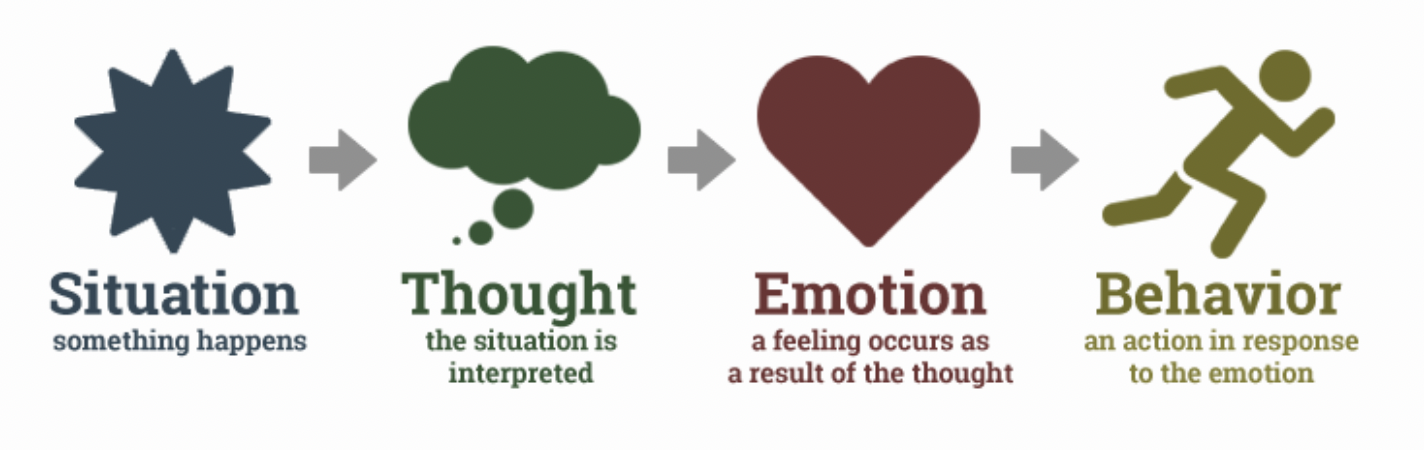
\includegraphics[scale=0.5]{images/cognitive-model.png}
    \caption{The cognitive model framework around which CBT is based \citep{therapist_aid_psychoeducation}.}
    \label{fig: CognitiveModel}
    \end{centering}
\end{figure}

CBT techniques are used to encourage deeper and more meaningful reflections from patients and provide them with alternative strategies to handle situations. These techniques are similar to those discussed to encourage reflections in learners about their graduate attributes. Development and improvement of these soft skills will benefit them in their future careers and improve their employability.

To explore if employing a CBT framework into the mobile app will encourage further stages of reflection, a case study was carried out to compare the results of users who were asked reflective job interview style questions with users who were asked CBT modelled questions. The results of this case study are discussed in chapter \ref{ExploratoryStudy}.

\section{Existing Products}

Similar existing products were researched and examined before the start of this project.

\subsection{Mahara - University of Glasgow}

University of Glasgow's site Mahara, \citep{mahara_dashboard}, was created to allow students to create a portfolio, and to adopt a habit of reflecting on the skills they have developed throughout university \citep{glasgow_university_attributes}.

\textbf{Advantages}
\begin{itemize}
    \item Users are able to make a page about anything, there is no requirement for their posts to be about their graduate attributes. The posts are freeform, they can be written text, audio, or video and include attachments and photos.
    \item It is a social blog website, allowing users to share their blog posts with their friends and tutors. Students are also able to join groups, creating 
    a community atmosphere. Users can choose to have their pages and posts set to private, giving users more control over their content.
\end{itemize}

\textbf{Disadvantages}
\begin{itemize}
    \item There are very few pages or posts, suggesting this site is not widely known by students, or students choose not to use it.
    \item The site is difficult to navigate, there are 'pages' and 'artefacts' but it is not clear how these are intended to be used, even after reading the 
    description of the site. 
    \item The site has a very basic minimalist design. This can be an advantage but, in this case, it does not have enough content to provoke engagement.
    \item Although users have freedom to create posts about any topic, this makes it less suitable in this context, where the focus is on graduate attributes, as found in the study by 
    \citet{mcdermott_developing_nodate}, it can lead to less reflections about students' graduate attributes.
    \item The site also does not provide the students with any guiding framework with which they can reflect on their learning, making it difficult for students
    to understand what to write.
\end{itemize}

\textbf{Overall}, this site has the potential to be used by students as a social blog about their learning and development throughout their time at university. However, there is a lack of novel and interesting design features and guidance to incentivise users to return to the website to make continuous reflections. It has limited use and is not ideal to encourage users to capture their reflections for the development of graduate attributes.

\subsection{Reflectly}

Reflectly is an app intended to capture users’ reflections on their daily lives in order to improve their mental health and wellbeing, through self-care and mindfulness. It makes use of positive psychology and CBT \citep{reflectly_app}. A unique component of the Reflectly app is the use of artificial intelligence to give users personalised questions and trends based on previous entries made. Although not designed to capture reflections on graduate attributes or learning, there are techniques and design features that are useful to analyse why this app is popular and enjoyable to use. 

\textbf{Advantages}
\begin{itemize}
    \item Allows reminders to be set to encourage users to reflect regularly.
    \item The app asks users aimed questions, for example "How can you reframe your worries?", this is helpful to users in understanding how to reflect effectively and provides a scaffold to support the user in their mental health development.
    \item Users are able to use different entry formats, they can create a written 'mood check-in', a voice recording, or a photo.
    \item The site uses conversational language to promote openness from the user.
    \item When inputting emotions, it asks the user to rate their emotions through a slider scale, meaning that the user does not have to identify specific emotions. 
    \item Questions allow users to choose from categories of reflection.
    \item The voice recording allows users to create a recording on any topic, the voice recording provides complete freedom for the user. This offers a good alternative to the written reflections where the users must choose a topic to reflect on.
    \item This voice recording capability uses voice recognition to create a written version of the note.
    \item The site provides motivational quotes to uplift users.
    \item The site uses enjoyable interface features that make the app colourful and interesting to use.
    \item The site provides useful links to resources that may assist the user in their reflections and improve their mental health.
\end{itemize}

\textbf{Disadvantages}
\begin{itemize}
    \item This app requires users to pay for a full subscription to use all of the available features, such as the artificial intelligence. 
    \item When users are carrying out a mood check-in, there is no framework to support the users understanding of their emotions.
    \item The voice recording capability converts voice recorded notes into written format, this does not allow the user to listen back to any recordings they have made and instead only keeps the written version. This could be inconvenient if a user would prefer to listen to their reflections.
\end{itemize}

\textbf{Overall} the app is a useful starting point for design for project app. However, Reflectly does not provide a framework to assist users in creating their own reflections. Further improvements could be made to direct users on the path of each stage of reflection to ensure they are creating meaningful reflections. Therefore, in the case of graduate attributes this would allow them to learn and develop these soft skills. Some features would be useful to implement in the project app, however, many of these features, such as the use of artificial intelligence to analyse trends in users’ entries, is not feasible within the scope of the project.

\subsection{Other products}

Other products that were examined were Catch It by \citet{nhsDigital_catch_2021}, and Daylio Journal by \citet{relaxio_src_daylio_2021}. However, these products focus primarily on mental health and wellbeing, and are generally less-fully featured than Reflectly. These products were therefore examined less thoroughly.

%==================================================================================================================================
\chapter{Exploratory Study} \label{ExploratoryStudy}

Through research into the development of graduate attributes and reflection, similarities were noted between CBT and graduate attribute reflection. The practices of CBT to create healthier and alternative ways to perceive a situation could be applied to graduate attribute reflection, providing a novel but appropriate theoretical framework for the project.

CBT could have several areas of application to assist students with their reflections on graduate attributes. CBT asks patients to reflect on previous experiences and to analyse their emotions and thoughts to become more aware of automatic negative thought patterns. Similarly, for students to be able to reflect effectively on their graduate attributes, they must analyse situations where they have exercised these skills in the past to become more aware of when they are using them and enabling positive 'reflection in action'. The questions used to provoke these deep reflections could potentially create a framework to assist students in creating equally meaningful reflections on both positive and negative experiences to help them develop and grow their graduate attributes.

CBT involves cognitive restructuring and reframing. It creates an awareness of negative thought patterns that a person does not realise they are experiencing and enables them to reframe these to be more positive. Similarly, Similarly, if graduates were made more aware of these skills and when they are using them then there is more opportunity to develop them. Furthermore, in any future situations they will be better equipped to understand the skills they require to benefit their work and environment and will be equipped to reframe the situation to be more positive and reflective.

Similarly to \citet{bruno_reflective_2018} stating that learners who work in a reflective environment develop a stronger degree of self-efficacy, people who undergo CBT are able to restructure how they view situations and develop a stronger sense of self-confidence. Employing these CBT techniques could have a similar impact on students and further increase their self-efficacy, restructuring their thinking process to utilise their skills in any given situation. 

Two important components of CBT are journaling thoughts and activity scheduling. Journaling allows the user to record their reflections, thoughts, and feelings, allowing patterns and tendencies to be identified and adapted \citep{ackerman_cbt_2017}. This will be the fundamental concept employed in the mobile app as it requires the user to take note of all of their reflections. Activity scheduling involves a participant noting something in their calendar that gives them anxiety. This cements the activity in their schedule and prevents later avoidance and decision making, helping to create better habits. This technique will be implemented as the app will provide reminders to encourage the users when to reflect, potentially creating a better habit of reflection.

It was therefore hypothesised that employing the techniques and questioning style of CBT could assist users in their reflections about their graduate attributes and lead to deeper reflections. This would lead to a greater development and situational awareness of these skills. To test this hypothesis A/B testing was carried out.


\section{A/B testing}

A/B testing was conducted in which a control group received job interview style questions, and the experimental group received questions using the CBT framework, these questions can be seen in Appendix \ref{Appendix-ABTests}. 

The control group was given interview style questions, as these lack any framework or guidance to support a person's reflection. However, this style of questioning is still intended to be sufficiently engaging to encourage a meaningful reflection on previous experiences, highlighting where and when skills have been shown by the interviewee. These questions would be a useful comparison as they simply ask the participant to reflect on the spot, whereas the experimental group is offered a CBT framework to support and lead their reflection, potentially encouraging deeper insight. Differences between these groups can be attributed to the CBT framework. 

The participants were a convenience sample of 10 students from the University of Glasgow. 5 participants identified as male, and 5 participants identified as female. These 10 participants were randomly assigned to one of the groups, either control or experiment group using \citet{random_lists_random_2013}.

After giving consent to take part in the experiment, participants were then directed to the corresponding Google Form which either asked the participant to reflect with the job interview style questions or the CBT style questions. These surveys can be seen in Appendix \ref{Appendix-ABTests}.

\section{Results}

To analyse the results of the A/B tests, the stages of reflection stated in Section \ref{backgroundReflection} were used. In each of the participants' answers, any comment that involved one of the stages of reflection was highlighted in a corresponding colour code, these colour-coded responses can be seen in Appendix \ref{Appendix-AB-responses}. These were then aggregated to show how many participants had engaged with each stage of reflection at least once during the case study, and placed in a graph to show the comparison of results with and without the use of CBT.

\begin{figure}[H]
    \begin{centering}
    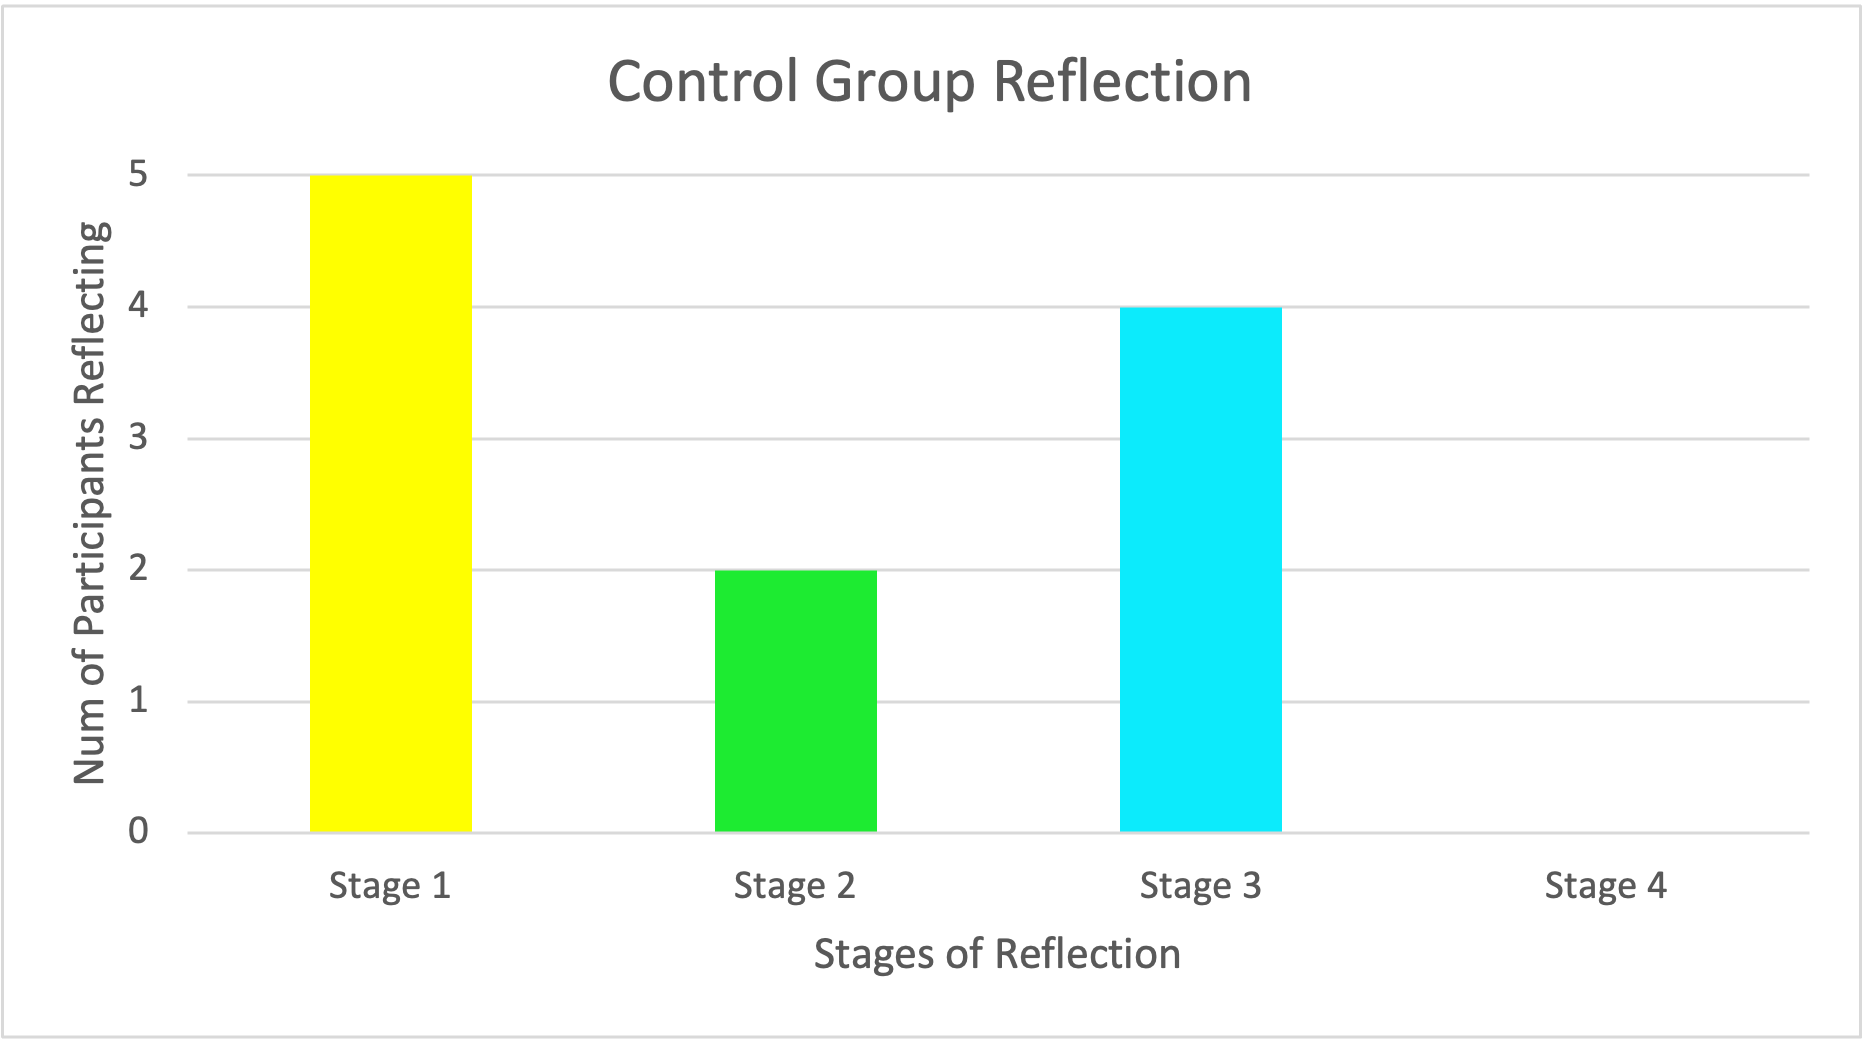
\includegraphics[scale=0.75]{images/ABControlGraph.png}
    \caption{The number of participants in the control group that carried out each stage of reflection. These participants were not given the CBT framework to encourage their reflection. It can be seen that most participants went through the first 3 stages, however, none of the participants carried out the final stage of reflection.}
    \label{fig: ABStudyGraphControl}
    \end{centering}
\end{figure}

\begin{figure}[H]
    \begin{centering}
    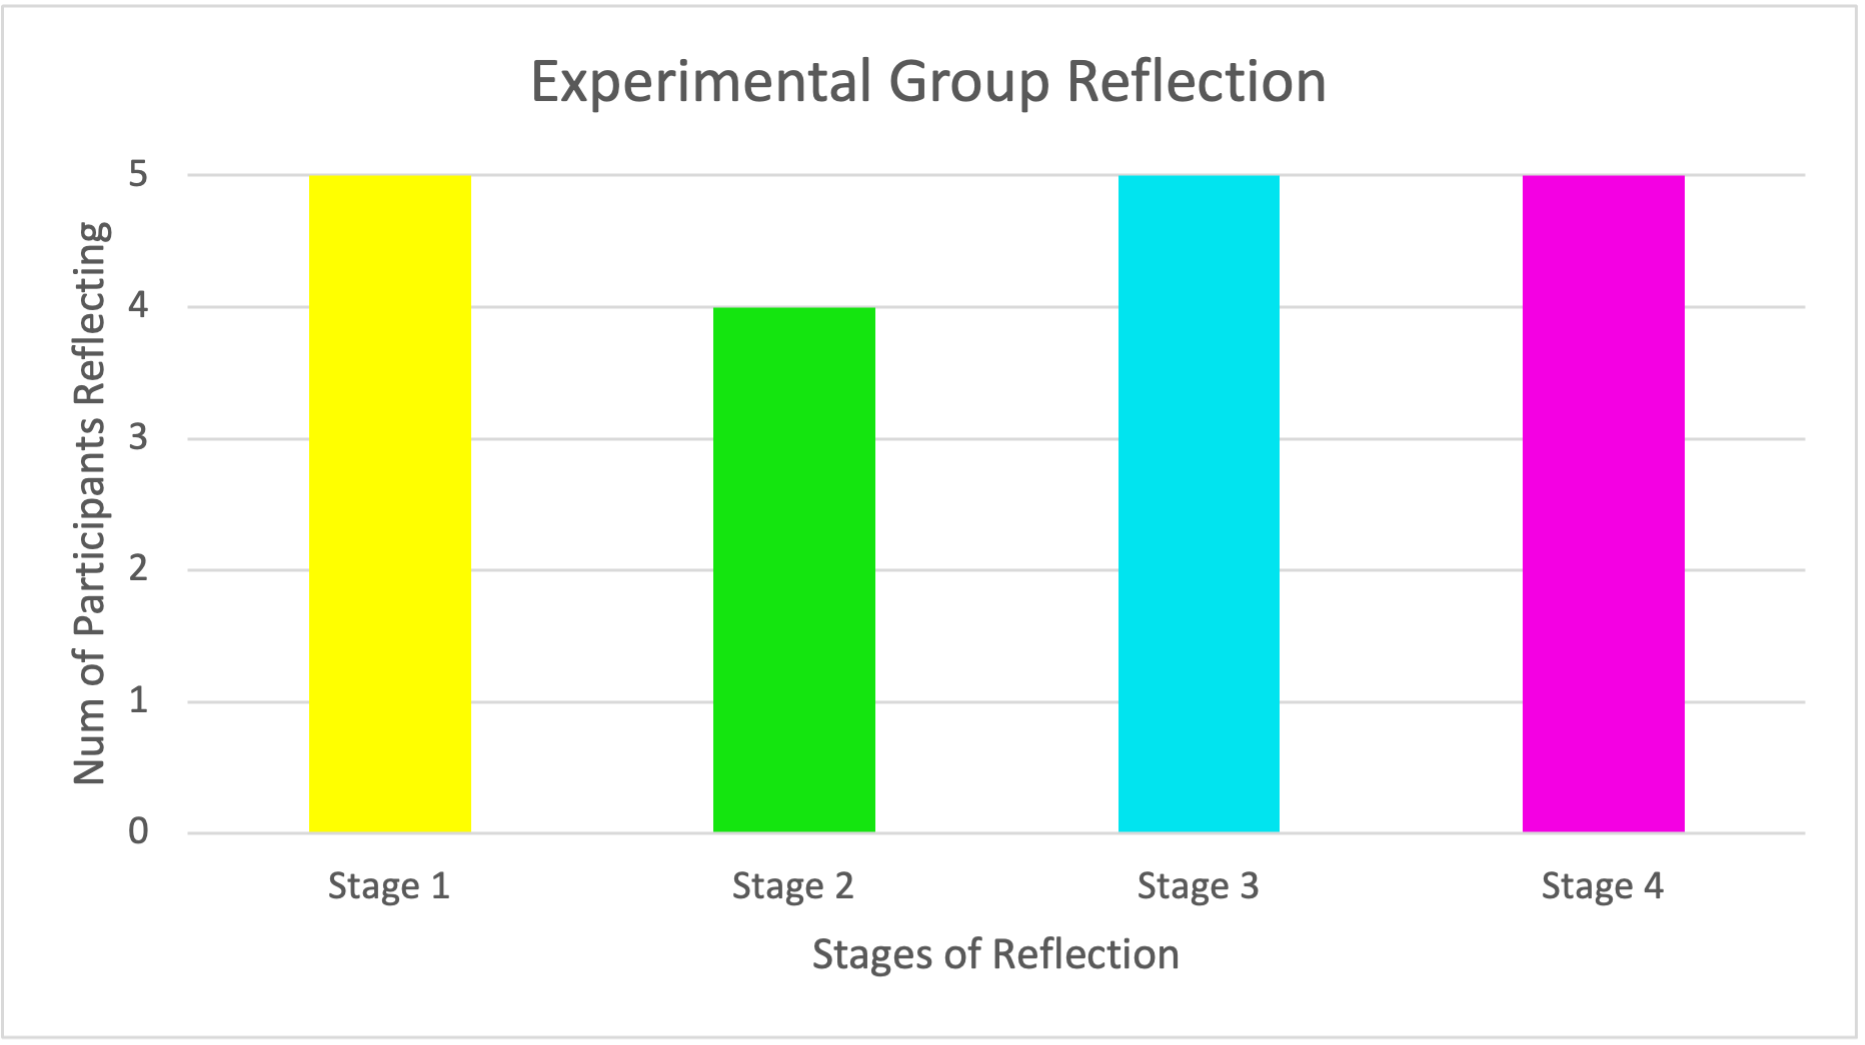
\includegraphics[scale=0.75]{images/ABExperimentGraph.png}
    \caption{The number of participants in the experimental group that carried out each stage of reflection. These participants were given the CBT framework to encourage their reflection. It can be seen that all bar one participant went through every stage of reflection in their answers.}
    \label{fig: ABStudyGraphExperiment}
    \end{centering}
\end{figure}

The results of the A/B test demonstrated that the participants given the job interview style questions were all able to carry out the first stage of reflection in which the person simply describes the concrete experience. This was also the case for the experimental group. 

Only 2 of the participants from the control group went through stage 2, in which the person describes the emotional state they were in during the experience, compared to 4 of the experimental group.

Stage 3 involves examining the cause and effect of the situation and how actions and behaviour affected the outcome. 4 out of 5 of the control group reached this level of reflection, whereas all 5 participants in the experimental group reached this stage.

Finally, for stage 4 of reflection, in which participants were expected to suggest alternative thoughts and behaviours and state if they obtained the best outcome, none of the participants in the control group reached this level. This distinctly contrasts with the experimental group in which every participant reached this level of reflection.

There is an observable difference within the results of the control and experimental group. These results clearly show that with the framework provided through CBT techniques, students were better equipped to have deeper and more insightful reflections on their graduate attributes. This CBT framework was able to lead students through each stage and encourage them to provide more cognitive analysis on the given situation. Furthermore, students in the experimental group had higher word counts for most answers. Although a higher word count does not provide evidence that further reflection is occurring, it can suggest deeper engagement with the process of reflection. 

Based on this sample of the student population, the results of the A/B test are in agreement with the statements made by \citet{bruno_reflective_2018} that state that students require clear instructions in order to reflect effectively, which the CBT framework can provide. The case study further suggests that CBT can lead to deeper reflections from students and should be integrated into reflective models in which students partake.


\section{Limitations}

Although this exploratory study was able to indicate that the use of CBT techniques and framework encouraged further reflection from students in this case, it cannot provide evidence of the long-term effects this form of reflection could have on students and how it impacts their graduate attributes. Also, due to the small sample size, these results are not generalisable and further in-depth research needs to be carried out. 

In future work, participants should be asked to answer these questions on a weekly basis for an extended period of time. Before conducting the experiment, users should be asked to complete survey instruments to assess their level of graduate skills and their confidence in reflection. This should then be compared with the answers they provide at the end of the experiment period to examine whether students had increased their level of development of their graduate skills and whether they felt more confident in their ability to reflect. The answers given on a weekly basis should also be examined to identify whether, over time, students were increasing their level of reflection in their answers. 

Such a longitudinal approach would allow conclusive evidence to be given on the benefits that the use of CBT framework could have on students and their graduate attributes. This, however, was not within the scope of the project due to time and resource constraints.
 


%-------------------------------------------------------------------

%==================================================================================================================================
\chapter{Analysis/Requirements} \label{analysis/reqs}

This project was presented by a University of Glasgow lecturer, Dr Matthew Barr, who required a mobile app to capture reflections on graduate attributes. A list of requirements was created in weekly meetings. This was an agile process where the newest version of the app, experiments, and design documents were presented and discussed each week. Dr Barr's book "Graduate Skills and Game-Based Learning: Using Video Games for Employability in Higher Education" provided enough detail to gain an understanding of what graduate attributes were and how they were learned \citep{barr_2019}. Lecture notes from the classes Mobile Human-Computer Interaction and Human-Computer Interaction were also used to gain understanding of how to create a usable and satisfying app for users, as well as how to conduct various evaluations and experiments that would be required for this project. Further requirements were gathered through personal heuristic evaluation as the project progressed, this allowed iterative improvements to be made to the app, increasing the overall usability.

\section{Problem Specification}

The main expectations for the app are listed below. The key requirement, as stated in the introduction, was to allow users to capture their reflections on when and where they have exercised their graduate attributes. It was decided that the best method to achieve this was to allow users to quickly and conveniently reflect using a mobile app. As the app will use Cognitive Behavioural Therapy techniques and prompts to encourage the user to reflect more meaningfully, they can, in their own time, deepen their understanding and development of these skills. The ability for users to make reflections easily was tested in the user evaluations in Chapter xx in the project. 

To begin creating the list of functional requirements of the GradReflect app, multiple user personas and user stories were initially created for students, interns/apprentices, recent graduates and experienced members in the workplace; these can be seen in Appendix \ref{Appendix-userPersonas} and Appendix \ref{Appendix-userStories}. However, in discussion with Dr Barr, it was decided the main users of this app would be students, and the app should be designed as such. The list of functional requirements below describes actions that users should be able to perform with the app. The list of non-functional requirements are criteria that the app needs to meet. These requirements follow the MoSCoW framework including Must Have (MH), Should Have (SH), Could Have (CH) and Won’t Have (WH) \citep{consortium_chapter_2014}. Requirements marked with * were added throughout the project as different iterations introduced possible new functionalities.


\textbf{Functional requirements}
\begin{itemize}
    \item \textbf{MH} Users must be able to capture a reflection of how and when they have exercised and developed their graduate skills; this can be in either written OR audio form.
    \item \textbf{MH} Users must be able to delete a reflection created, as well as being able to review it at a later date; however users should not be able to update or edit a note after its creation. 
    \item \textbf{MH} Users must be able to turn on notifications.

    \item \textbf{SH} Users should be able to select a skill from a pre-defined list to avoid mistakes and allow for future potential filtering.
    \item \textbf{SH} When creating a written note, there should be help buttons that explain to the user how they should answer each questions and provide an example, this will give them clear instructions to allow effective reflection.
    \item \textbf{SH} Users should be able to give their note a title to allow for clear representation of what a note contains, and allow for future potential searching or filtering.
    \item \textbf{SH*} Users should be able to create a reflection in BOTH written and audio form. This will allow both structured reflections and freeform spoken reflections for convenience. 
    \item \textbf{SH} The app should contain a description of each of the skills that users are expected to develop and reflect on during the use of the app. 
    \item \textbf{SH*} Users should be able to search for the name of a note or a skill category to filter the notes in the list by skill.
    \item \textbf{SH} The app should have a Settings page to view information about the app.
    \item \textbf{SH} GradReflect should have an About Page within the settings that tells the user how to use the app correctly to make reflections, giving further clear instructions to the user. 
    \item \textbf{SH*} Users should be able to view statistics based on the reflections written into the app.
    
    \item \textbf{CH} The app could implement Cognitive Behavioural Therapy techniques to aid reflection and provide users with a suitable framework to support them and provide clear instructions on how to reflect. 
    \item \textbf{CH*} Users could have the ability to customise their experience of GradReflect and have the ability to switch between a dark and light themed interface.
    \item \textbf{CH} GradReflect could have links in the Settings page that take users to useful pages related to the app and graduate attributes to provide further insight and education on graduate attributes.
    
    \item \textbf{WH} It was decided that users will not be able to upload reflections onto Moodle as this does not provide enough benefit to users in completing the aims discussed in Section \ref{IntroAims}. There could also be potential privacy issues, as users may not want to upload personal experiences on a public space.
\end{itemize}


\textbf{Non-functional requirements}
\begin{itemize}
    \item \textbf{MH} Must be intuitive and easy to use. An app that is easier for new users is more likely to encourage interest in it.
    \item \textbf{MH} Must help users to create meaningful reflections about their graduate skills. The ability for users to reach more stages of reflection will help develop these skills.
    \item \textbf{SH} Users should be able to create quick reflections.
    \item \textbf{SH} The app should encourage users to continue using the app in the future.
    \item \textbf{SH} Users should find the features of the app useful and find the value in using an app like this to reflect. 
\end{itemize}


\section{Chosen Limitations}

Due to this app being designed and created for iOS devices, users will not be able to download this app onto their own device without the app being uploaded to the Apple App Store \citep{apple_inc_app_2021}. This would require a paid Apple developer license and is therefore out with the scope of this project. This meant that some limitations were chosen to create a prototype of the app to test and evaluate the app, that in the future could be taken onto other platforms and for general distribution.

Reminders will not be able to be set by the user, instead they will turn on the notifications and a notification will launch after 10 seconds. This was for ease of testing. The response time of notifications was therefore immediate and as the app will be run on a simulator that is not always running, test users will not be able to use GradReflect for extended periods of time that would allow a notification to be set in the future. In future developments of this app, users would be able to turn on notifications and the notifications would remind the user to reflect once a week on their chosen day.


\section{Changes to the Specification}

The specification was changed in discussion with the project supervisor, as described at the beginning of this chapter, due to project constraints and novel research paths that opened up during these conversations. The main change to the original specification given was to integrate CBT techniques into the app. This was chosen during research into situations where people reflect deeply and meaningfully about their real-life experiences. This was framed as a research question for the project, to evaluate its possible benefits in aiding the reflection of users about their graduate attributes. 

Each possible feature of the app was also evaluated based on its usefulness. As a result, the decision was made to remove the ability for users to upload their reflections to Moodle. Due to the research direction of CBT users will include their thoughts and feelings into their reflections, causing it to be more personal. Upon conversation with peers, it was also noted that students would be unlikely to use this feature. The decision was then taken to include a link to Moodle on the Useful Links section of the mobile app instead, to maintain a connection with the university and the app.


%==================================================================================================================================
\chapter{Design}

This chapter discusses the design of the product, starting with the design of the CBT-based reflection techniques. The user interface design will also be discussed, including the reasoning behind a number of key design decisions made to meet the requirements laid out in \ref{analysis/reqs}. Finally, the chapter will examine the tools and technologies used for the project. 

\section{Encouraging Reflection}

In order to encourage reflection, various use cases and features were designed to give users more reasons to use the app.

\subsection{Written Notes}

The ability to enter written notes was required to give users the opportunity to reflect using the CBT methods described in Chapter \ref{Background}. The questions would be designed similarly to the questions used in the experiment described in chapter \ref{ExploratoryStudy}, with only minor alterations to allow more functionality within the app. 

Each question was required to be stated clearly and concisely, with a help button displayed to provide insight into answering this question with an example. This will allow the user to understand what the app is expecting of them and further encourage deep and meaningful reflections as they have been given the required instructions needed to do this \citep{bruno_reflective_2018}. This additional explanation of the questions are also in line with Nielsen’s ‘Help and Documentation’ heuristic \citep{Nielsen10}. The CBT-based questions and prompts that were designed and subsequently implemented into the app, can be seen in Appendix \ref{Appendix-AppCBTQuestions-Prompts}.

The question on emotional reaction was designed to utilise a sliding scale from a clear negative reaction to a positive reaction. This meant that users were not required to label an emotional response, which can at times be difficult to identify. 

Users were also given the opportunity to be able to click on previously made notes to review, reflect on, and delete. However, they were not able to edit or update any of their reflections. This mirrors the CBT behaviours of writing down reflections in a journal where they cannot be altered retrospectively. This prevents hindsight on previous experiences and ensures an accurate contemporaneous representation of experiences.


\subsection{Recorded Notes}

Users were provided the option of creating a note through a voice recording. This would add further convenience to quickly reflect, recording an experience that they may wish to return to. There is no framework provided when creating a recorded note, allowing users the freedom to reflect however they want. The ability to say what is on their mind allows free contemporaneous vocal notes, rather than arranging thoughts into a cohesive written sentence.

\subsection{Statistics}

Statistics on a user's written reflections were developed, providing detail on data holistically and organised by skill. The user is able to view how many notes they have made and the average words per note. They can also scroll through each skill to see how many notes they have written, their average words per note for that skill, and their average emotional response for that skill. This feature allows users insight into their own reflections, focusing on their development of skills.  

These insights will allow the user to see both their strengths, through the skills with a high number of notes, and their potential weaknesses, through skills with a comparatively low number of notes. This focusses their goals, showing where future development is required. It also shows users where they may need to reflect more deeply through the word count. If the word count is low, it is likely they not spending enough time reflecting or reflecting in enough detail. And lastly, they will gain insight into how they feel about certain skills. If their average emotional response to a skill is low, they can evaluate the reasons for this, potentially allowing for future development of this skill.


\subsection{Additional Assistance}

Additional assistance for reflection was also designed into the homepage and the settings page. Upon entering the app, users should be greeted with descriptions of each skill and an example of its use. Descriptions of the skills help to educate the users, due to the gap in the knowledge of these skills identified in the graduate attribute survey conducted at the beginning of the project, which can be seen in Appendix \ref{Appendix-gradAttributeSurvey}. Clear descriptions and instructions of the skills will increase a user’s awareness of these skills in their everyday life.

Further descriptions of how to use the app are given within the settings page, increasing the level of clear instructions needed to help students be able to reflect effectively \citep{bruno_reflective_2018}.


\section{User Interface}

The user interface was designed to help users quickly learn how to use the app and start reflecting. To do this, it was required that the interface was intuitive and easy to use, this would be made possible through an attractive and straightforward design. This section describes some of the techniques used during that design process.

\subsection{Initial Prototyping}

In order to gain insight into what each page would require and ensure all features had been considered, all designs went through a prototyping process. 

Design of existing note taking apps were considered for interface familiarity. Some of these similarities are listed below.
\begin{itemize}
    \item Title of the view stated in bold at the top.
    \item A search feature at the top of the view.
    \item Notes in a listed format with title and date created displayed.
    \item A return button at the top left corner of the view.
    \item An edit button, or swiping functionality on a specific note, to delete notes.
    \item Recordings page with a large recording symbol at the bottom of the view.
    \item A settings page containing the creation details, customisation of the app and further information about the app.
    \item TabViews, native to iOS, containing information or images that users can scroll through, containing small dots at the bottom to show which tab the user is on.
\end{itemize}

Some of the apps referenced for this were: Apple's Voice Memos \citep{apple_inc_voice_2021}, Apple's Notes \citep{apple_inc_notes_2021}, Google's Keep Notes \citep{google_llc_google_2021} and Collateral \citep{vargas_collateral_2021}.

External consistency allows users to feel more comfortable and understand the app better as it is similar to those they have used in the past, and follows Nielsen’s heuristic ‘Consistency and Standards’ \citep{schlatter_visual_2013, Nielsen10}. This helps to satisfy the requirement that the app be easy to use. 

Appendix Figure \ref{fig:PaperPrototype1} shows the initial paper prototype developed for GradReflect. A homepage design that directed users to each section of the page was first envisioned. This homepage would provide users with descriptions of each skill and how to use the app. Initially, skills would only appear on a user’s first time using the app, and then would be held within the settings section of the app. However, prototyping suggested that it was more helpful if the skills were always available on the home page. This would aid users to instantly understand what to do on first opening the app, but if users have used the app several times, they are able to head quickly to the section they wish to use, whilst also having the available the skill descriptions if users want to refresh their knowledge. This meets the standard of Nielsen’s heuristic ‘Flexibility and efficiency of use’ \citep{Nielsen10}.

Paper prototypes were subsequently created for the remaining views of the app with a similar design to the homepage for consistency, as seen in Appendix Figure \ref{fig:PaperPrototypes}. This prototyping stage was extremely valuable and assisted in speeding up the implementation stage as the design decisions had already been carried out, giving a clear idea of how the final product should appear, ensuring the requirements would be met. However, some alterations were made to these designs for the final implementation. 

These designs were then implemented into high fidelity wireframe prototypes, using iOS design features, these can be seen in Appendix \ref{Appendix-highFidelityWireframes}.


\section{Technologies}

The technologies used and the reasons behind those choices are described.

\subsection{iOS Mobile app}

A mobile app was chosen, as the project did not require user accounts or the external information sharing that is made easier by using web frameworks. Due to the personal nature of the reflections being carried out by users and the use of CBT, the ability to carry out these reflections on their phone can lead to more intimate and personal reflections. Additionally, as these reflections are on personal experiences, it is convenient for the user to be able to carry out reflection on-the-go on their mobile device, allowing instant reflection to be captured of events, thoughts, and emotions. 

iOS was chosen due to familiarity with the platform and appealing interface design concepts.

\subsection{iOS Development}

Apple's iOS development is exclusive to Apple devices. Creating an iOS app for any platform; Mac, iPhone, iPad, Apple Watch, or Apple TV, requires the Apple \textbf{XCode IDE}. 

\textbf{Swift} is the language used to create mobile iOS apps. It is a modern language with inferred types making it less prone to mistakes, and syntax that encourages clean and concise coding. This syntax, although appearing strict at times, allows for safeguarding and prevention of errors, improving readability with its similarity to natural English \citep{altexsoft_swift_2021}, and allows for easier learning of the language and start to development.

\textbf{SwiftUI} was chosen for the interface development. SwiftUI is a new and innovative way to create interfaces that can allow for entire apps and their functionality to be written using it \citep{apple_developer_xcode_2021}. It uses declarative syntax to allow a developer to simply state what they want the interface to do. A key benefit to using SwiftUI is the preview editor that adjoins the code editor, displaying the app for any device and orientation. As code is written it is instantly compiled and the preview shows live changes \citep{apple_swiftui_2021}. These benefits allow for easier creation of the app's interface and its functionality, assisting in creating a more visually appealing and clean interface.


%==================================================================================================================================
\chapter{Implementation} \label{implementation}

This chapter describes the steps taken to implement the mobile app GradReflect, and the technical decisions that were made during this process.

\section{User Interface}

The user interface was implemented using SwiftUI with an aim to make it easy to use and visually appealing. 

\subsection{Model View ViewModel}

SwiftUI presents both useful features and challenges when creating an app. Instead of a typical Model View Controller design pattern, SwiftUI is state-driven and declarative, implementing a Model View ViewModel design pattern built into the framework \citep{naumov_swiftui_architecture_2019}. Tutorials from CodeWithChris \citep{ching_codewithchris_2021}, SwiftUI Masterclass Course \citep{petras_swiftui_2021} and Blckbirds \citep{blckbirds_learn_2021} were used to learn the basics of SwiftUI development and begin implementation.

\textbf{Model:} The model classes within SwiftUI are used as a data container that define a structure that will be written to and fetched from. An example of this is the Skill Model. This defines that each skill contains an id, a title, description, an image, and gradientColours which defines the colour scheme for that skill card. This model is also reused for the Statistics view.

A model was also created to hold the note entries created by the user via Core Data, the permanent storage that organises the data in an entity-attribute relationship. Core Data is an aspect of iOS development that involves a steep learning curve, however, it proved to be beneficial. This was due to the ability to manipulate the data within the fetch request in a single line of code, and its ability to track changes through the persistent storage. This made for greater simplicity during implementation. Core Data is saved using an NSManagedObject which uses optimised storage and retrieval methods with key-value coding and observing. This is faster than other means of storage and retrieval, including get/set methods \citep{apple_developer_documentation_core_2021}. Core Data entry is operated via the ViewModel, translating user events received from the view into CRUD (create, read, update, and delete) operations that can change the model and its data. The flow of data can be seen in figure \ref{fig:MVVMDataFlow}. 

\textbf{View:} The view is responsible for displaying the UI and animations. A secondary responsibility of the view is to receive any user interactions and pass these to a view model for interpretation \citep{bulavin_modern_2020}. The view is made up of views and controls; each view represents a building block of user interface. The controls allow the user to interact with this interface. SwiftUI made it straightforward to build a UI, allowing the standard building blocks to be altered to fit the needs of the project concisely and simply, making this aspect of implementation rapid.

\textbf{ViewModel:} The ViewModel is responsible for dictating how data should be represented in the view, as well as interpreting user inputs into actions and updating the UI state and behaviour accordingly. The ViewModel can take the form of the @State variables bound to the view, updating the UI anytime changes are made to the state. These ViewModels can also take the form of a distinct ObservableObject class. As an example, the Router class is a ObservableObject class, this handles when a view's StateObject 'current page' variable will change, and updates the view to show the requested page.


\begin{figure}
    \centering
    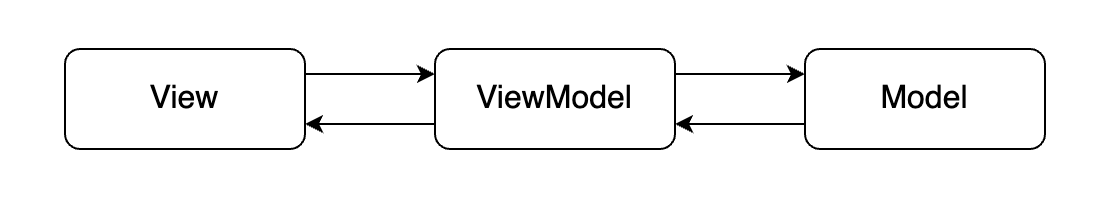
\includegraphics[scale=0.5]{images/MVVMDataFlow.png}    
    \caption{This diagram shows the data flow between components in the Model View ViewModel (MVVM) design pattern 
    \citep{bulavin_modern_2020}.}
    \label{fig:MVVMDataFlow} 
\end{figure}


\section{Aesthetics}

\subsection{iOS Native Appearance}

SwiftUI enforces a standard design of common on-screen objects. These were found to be very user-friendly and attractive, with only a minor issue highlighted in the usability study in section \ref{evaluation}, where users attempted to delete a note within the review view, instead of using the edit button on their first attempt. Another advantage of the SwiftUI framework is that it allows for the creation of existing iOS features, such as the Edit button, to give a cohesive and familiar appearance on iOS devices. This was beneficial as it meant that there were pre-built buttons with pre-written functionality. It also allowed the project to focus on the problems specific to the aims of the project, instead of the detailed aspects of the design. However, it also meant that this code was not able to be altered to adjust functionality. The user interfaces for the main views of the app can be seen in Appendix \ref{fig:appMainViews}.

\subsection{Aesthetic Features}

\textbf{App Icon and Logo:} An app icon was created with associated logo for launching the application from the app library. This creates a professional and attractive first contact with the app. This can be seen in Appendix Figure \ref{fig:AppLogo}.

\textbf{Loading Screen:} A loading screen was created using the app’s logo and colour scheme. This was to create a more professional and attractive looking app, whilst also performing the function of assuring the user that the app is loading, instead of a generic white screen which could lead the user to believe the app had crashed.

\textbf{Emojis:} Emojis were implemented throughout the app. This was suggested by a potential user during early stages of development. This created a more casual and friendly design to the app whilst also being informative of functionality. These emojis can be seen in the titles for views in Appendix \ref{fig:appMainViews}.

\textbf{App information in Settings:} Detail about the app such as name, compatibility, developer, version and created date are provided in the settings section of the app. This is a common feature in iOS apps and gives a more professional design, seen in Appendix \ref{fig:appSettingsScreen}.

\textbf{Images on skill cards:} Each skill card contains a graphic that summarises the skill, seen in Figure \ref{fig:AdaptabilitySkillCard}. These make the app more attractive and add to a user's understanding of a skill. Many users indicated they enjoyed these images in the user evaluations (Chapter \ref{evaluation}).

\textbf{Toggle dark/light theme:} Users are able to toggle between dark and light theme within the app. This provides an element of customisability to the app for users, adding to usability and attractiveness. This dark mode can be seen in Appendix \ref{fig:DarkMode}, compared with the light mode that can be seen in Appendix \ref{fig:appMainViews}.

\begin{figure}
    \centering
    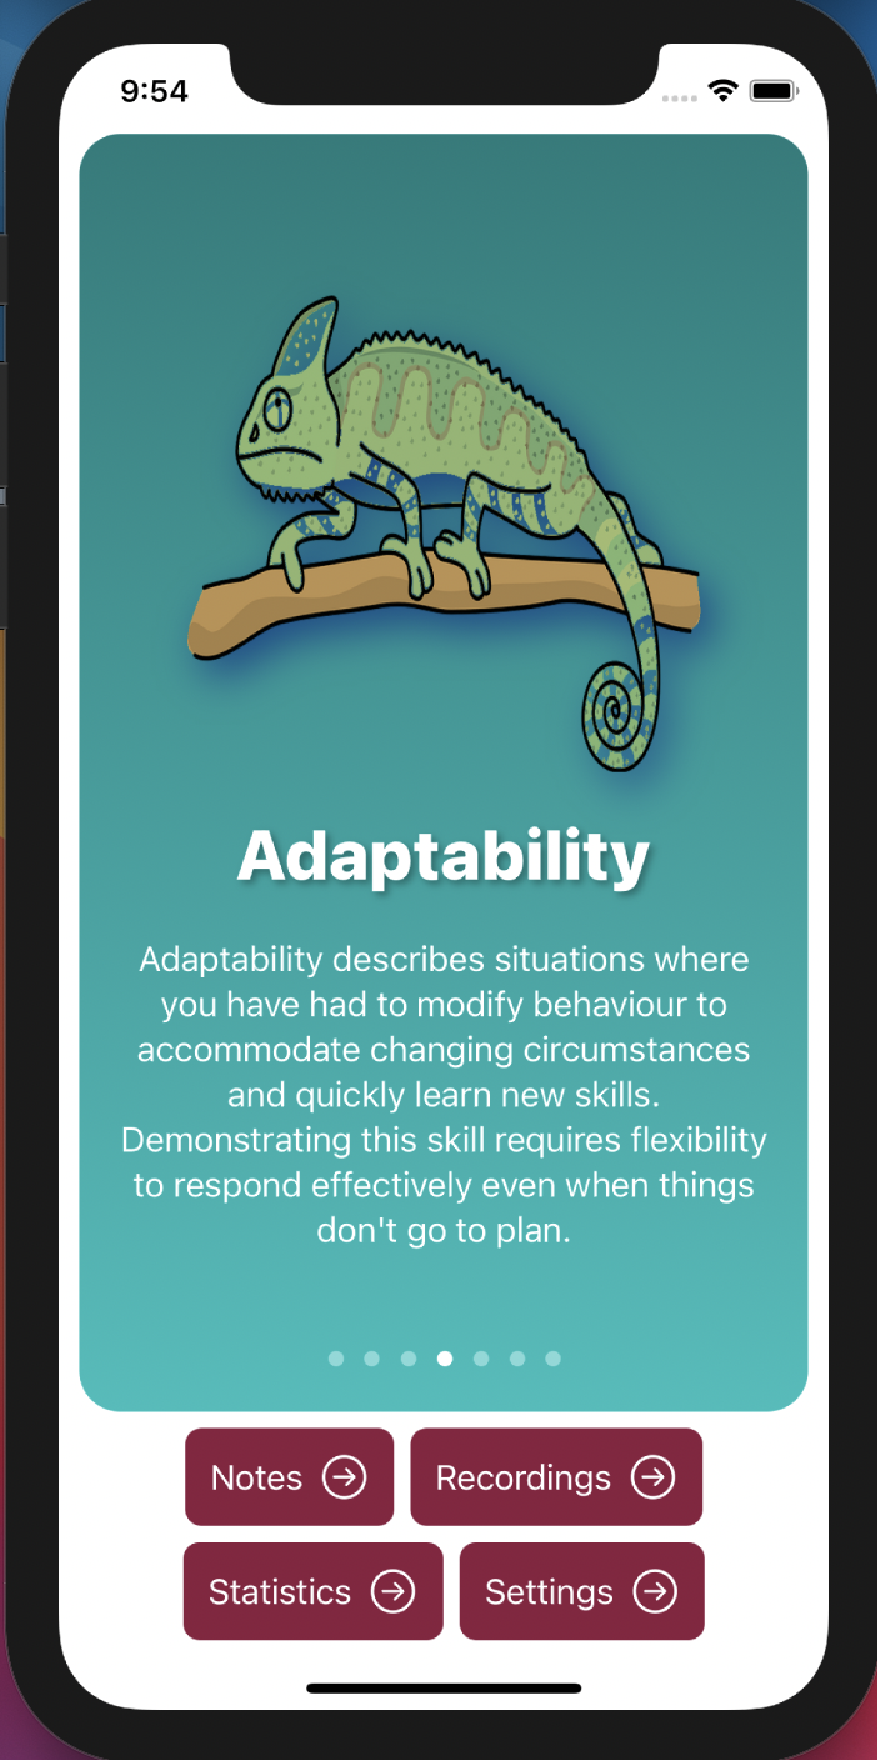
\includegraphics[scale=0.3]{images/AdaptabilitySkillCard.pdf}    
    \caption{This screenshot shows the Adaptability skill card, one of the 6 skill descriptions available on the Home view of the GradReflect app.}
    \label{fig:AdaptabilitySkillCard} 
\end{figure}

\section{Features}

This section describes how the functional requirements for the system were implemented and lists some of the most important and relevant features. 

\subsection{Learn About Graduate Skills}

It is important for those who want to reflect and develop their graduate attributes to learn and understand what these skills are. By knowing what these skills are, users are more comfortable in their reflections, and having the skill cards in the home section of the app with a helpful graphic and description of the skill will facilitate this. Each of these skill cards can be seen in Appendix Figure \ref{fig:AllSkillCards}, the first of which is the Home Card that describes what each area of the app is used for. These skills descriptions, on the home section of the app, allow new users to instantly scroll and familiarise themselves with the skills they are looking to develop. Experienced users do not have to scroll and can immediately choose where they want to navigate, while still having the option of a convenient reminder should they require it. The colours used in each of these skill cards was made to be compatible with the colour scheme used in the app logo using the website Coolers \citep{coolersco_coolors_2021}.

\subsection{Creating and Deleting a Note}

The ability to capture a reflection in written form was a key functional requirement for this project. This project stands out from similar existing note or reflective apps with its utilisation of CBT techniques providing the framework needed to support users in this reflection. This was implemented through the note creation form. Users are able to create and save a new note using the question prompts provided for them, as seen in Figure \ref{fig:CreatingNote}. This aims to give clear instructions to focus the user on reaching all stages of reflection. 

The user is also supported in their reflection through the use of help buttons. The user is able to click on the '?' button next to any of the questions in the note entry form and an alert will appear that provides further detail on how they are expected to answer the question. An example of this alert can be seen in Figure \ref{fig:HelperButtonAlert}. Throughout each of the help button alerts, the example of a communication skill reflection is used where someone has had to settle a dispute in their team. Examples are given in each of the alerts using this situation to demonstrate the reflections the user could make. All CBT-based questions and helpful prompts can be seen in Appendix \ref{Appendix-AppCBTQuestions-Prompts}.

Users can select one of the 6 skills available to reflect from a picker, ensuring conformity in the skills ensuring there are no issues when users later search for a skill to filter their notes list. Users are also able to select their emotional response to a situation using a slider, simplifying this reflection for them. 

Users are able to save a note after reflecting, requiring at least a title. This was intended to give the user freedom in how much they did or did not want to write as they could leave some entry fields empty. They are also able to cancel a note at any given time by either clicking the cancel button or swiping from the top down to dismiss the form. 

Users can later delete a note by either selecting the edit button, or through swiping a note in the list to the left. The edit mode for notes can be seen in Appendix \ref{fig:DeleteNote}. This is a native gesture in iOS used frequently in other apps. Users are unable to update or edit a note after its creation.


\begin{figure}
    \centering
    \begin{subfigure}[b]{0.3\textwidth}
        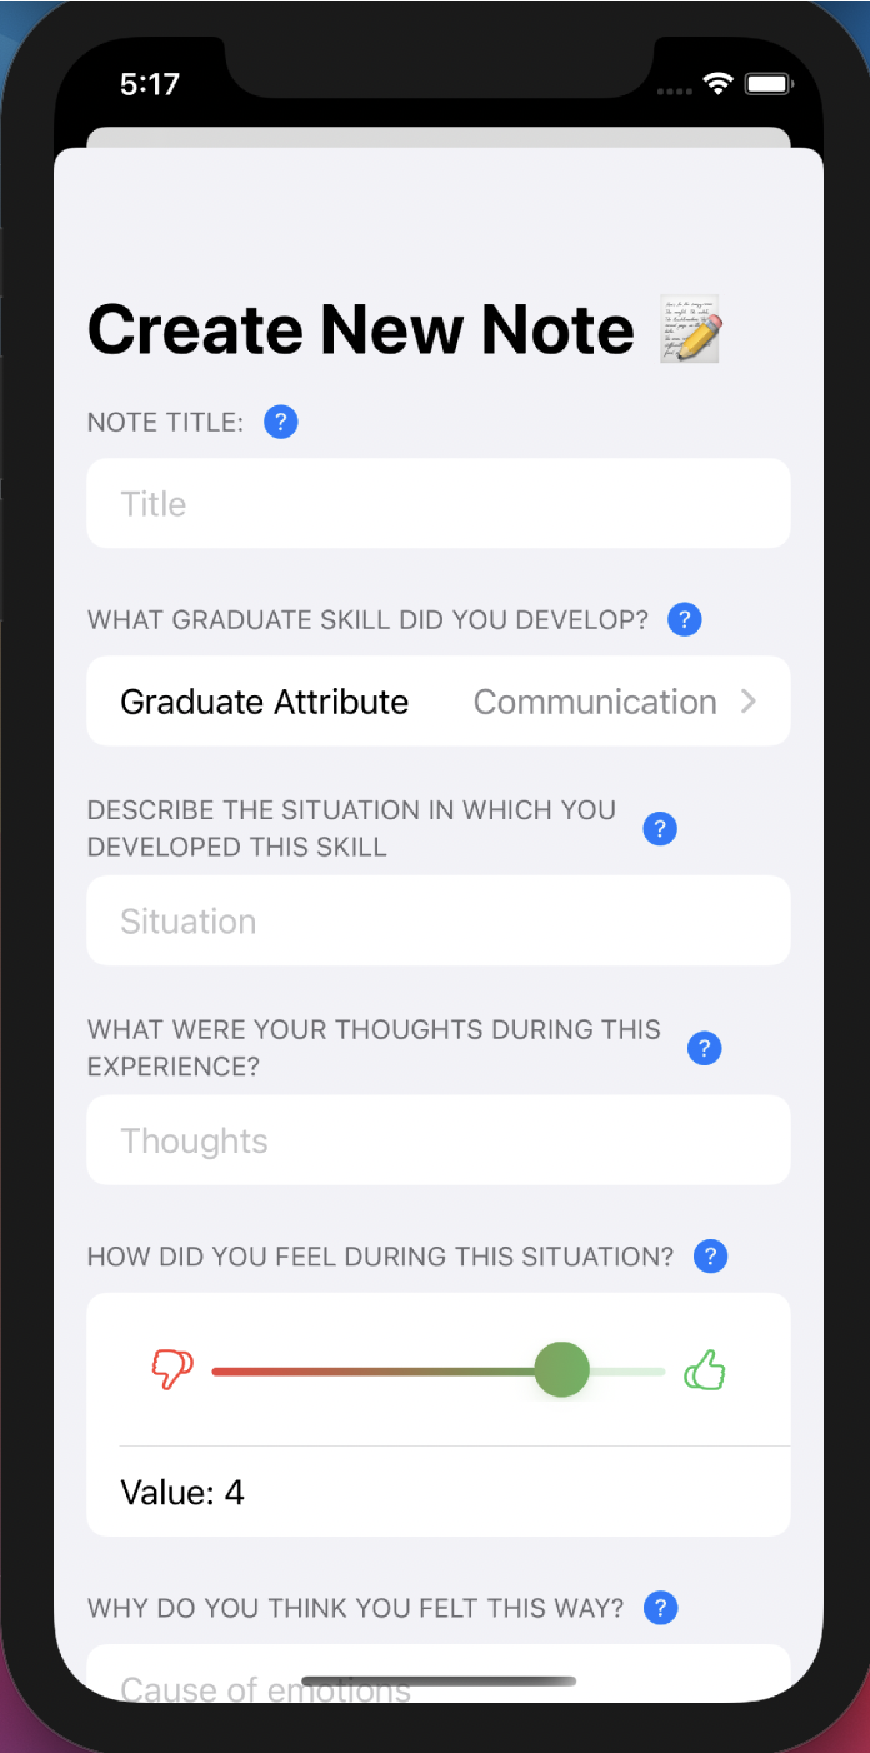
\includegraphics[scale=0.25]{images/CreatingNote.pdf}
        \caption{Form to create a note.}
        \label{fig:CreatingNote}
    \end{subfigure}
    \begin{subfigure}[b]{0.3\textwidth}
        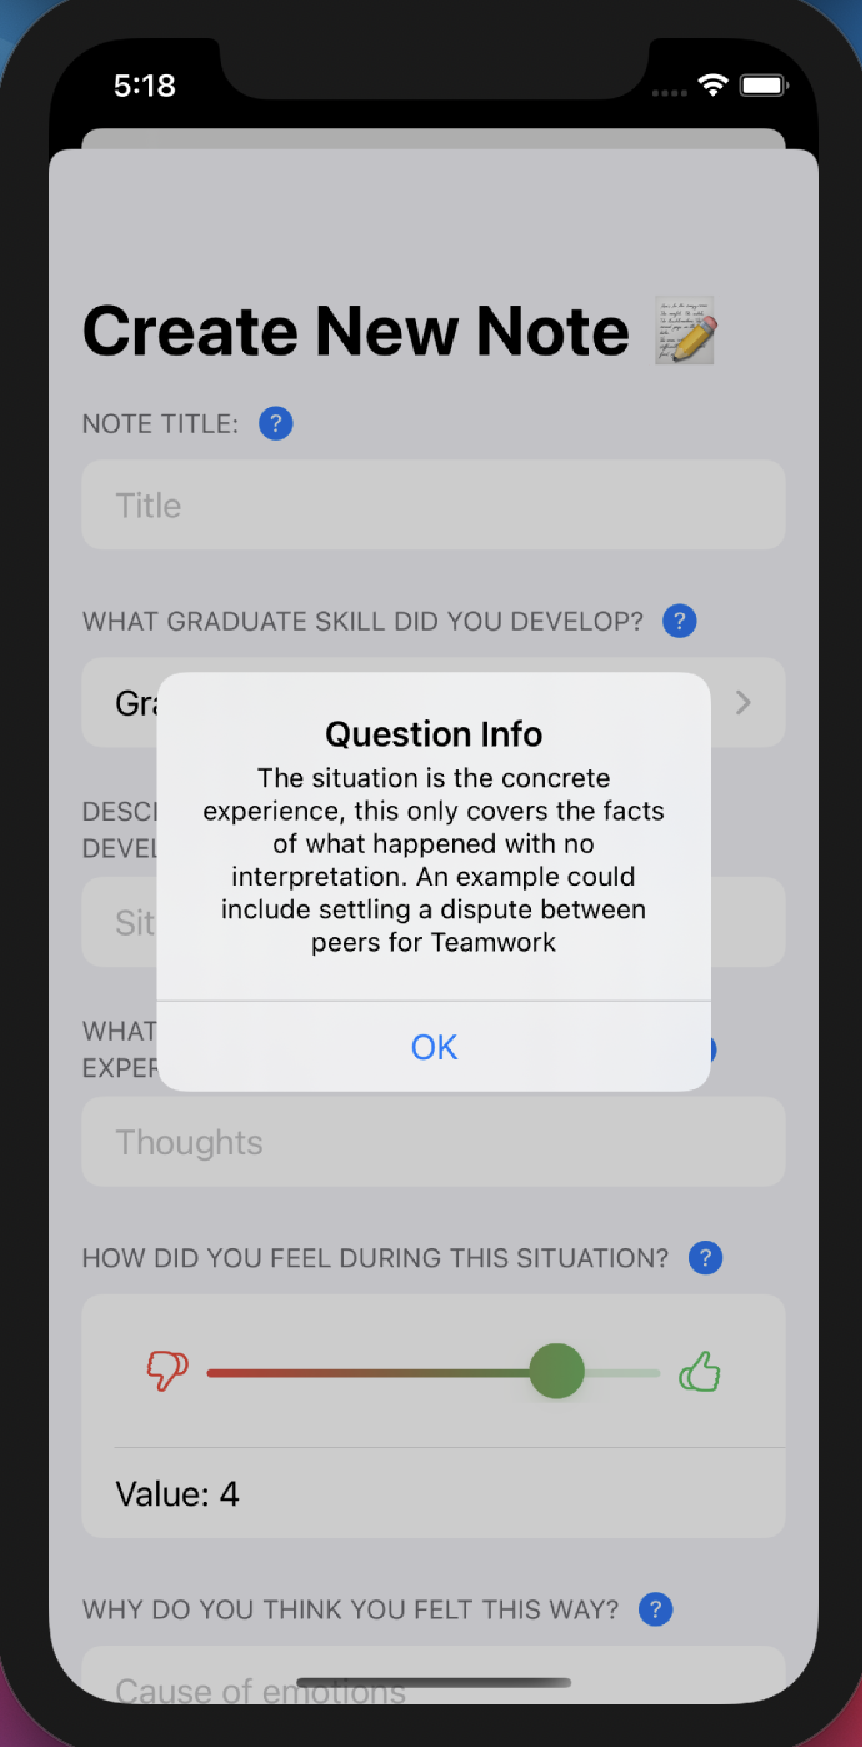
\includegraphics[scale=0.25]{images/HelperButtonAlert.pdf}
        \caption{Alert given from the situation prompt by help button.}
        \label{fig:HelperButtonAlert}
    \end{subfigure}   
    \begin{subfigure}[b]{0.3\textwidth}
        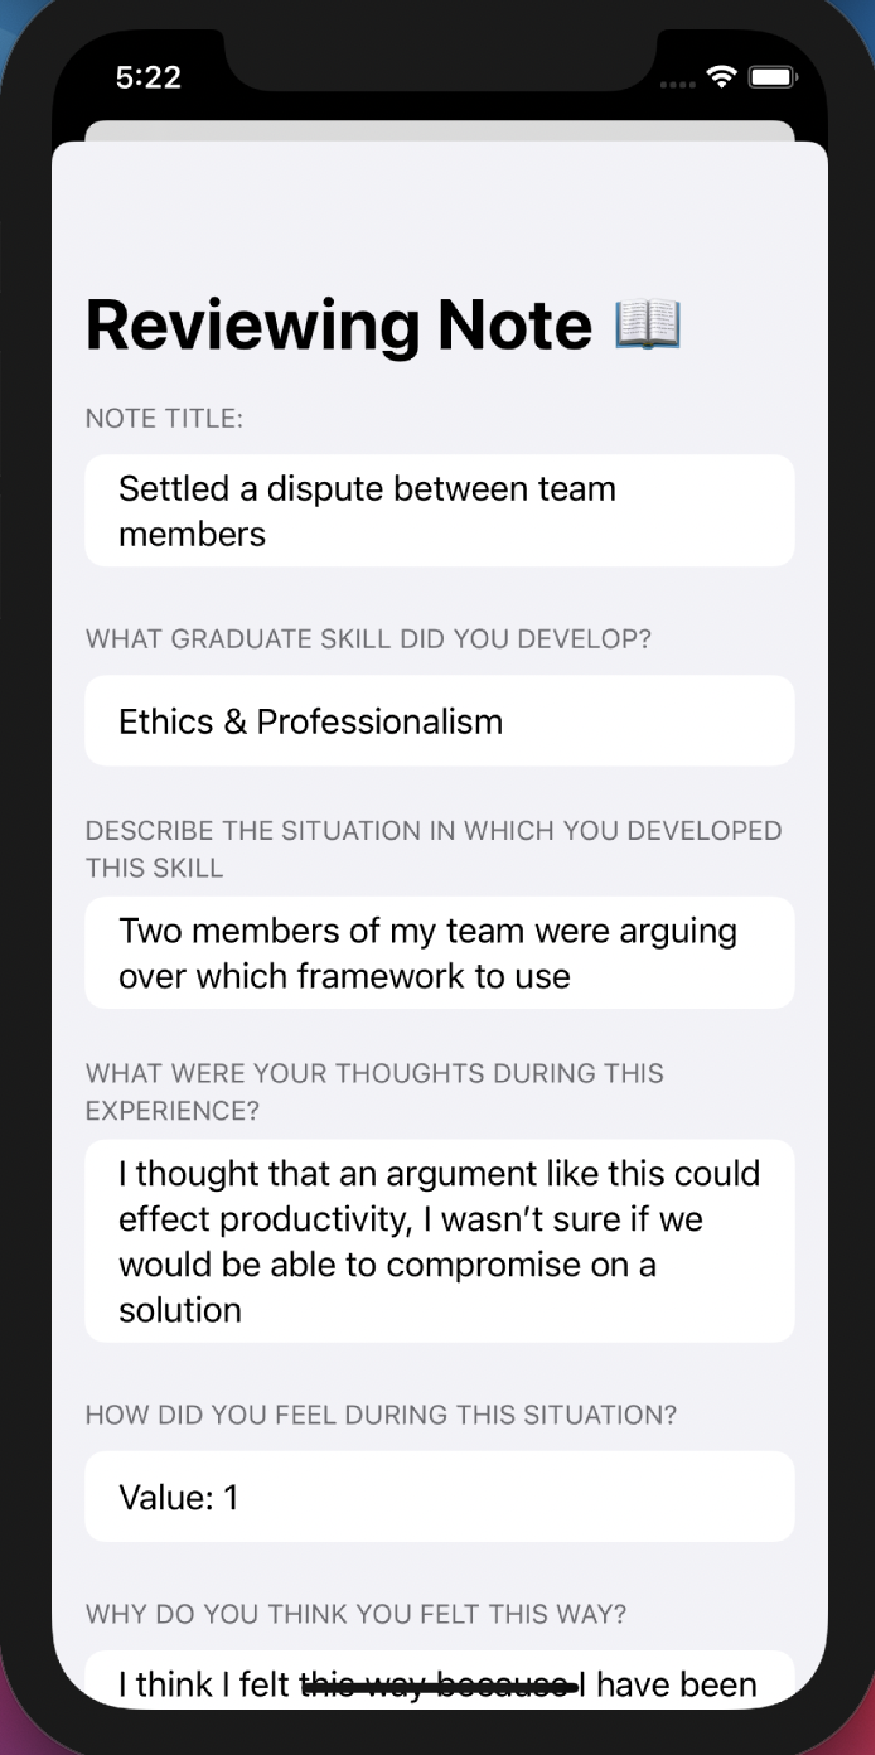
\includegraphics[scale=0.25]{images/ReviewingNote.pdf}
        \caption{Reviewing a note}
        \label{fig:ReviewingNote}
    \end{subfigure}   
    \caption{Screenshots showing the views when creating a note and reviewing it.}
    \label{fig:NoteCreationReview}
\end{figure}

\subsection{Reviewing a Note}

Users are able to click on a previous note they have made, allowing them to reflect on previous entries. This could enable them to see how they have improved or handled previous similar scenarios. This can be seen in Figure \ref{fig:ReviewingNote}.

\subsection{Search and Filter}

Users are able to type in the name of a note to filter the list of notes presented, shown in Figure \ref{fig:SearchFilter}. They are also able to type in a specific skill to filter the list by that skill. This is a useful feature as it is intended that users would continue to use this app frequently to reflect, and therefore having the ability to filter notes would make it easier for them to find previous notes they have made.

\begin{figure}[H]
    \centering
    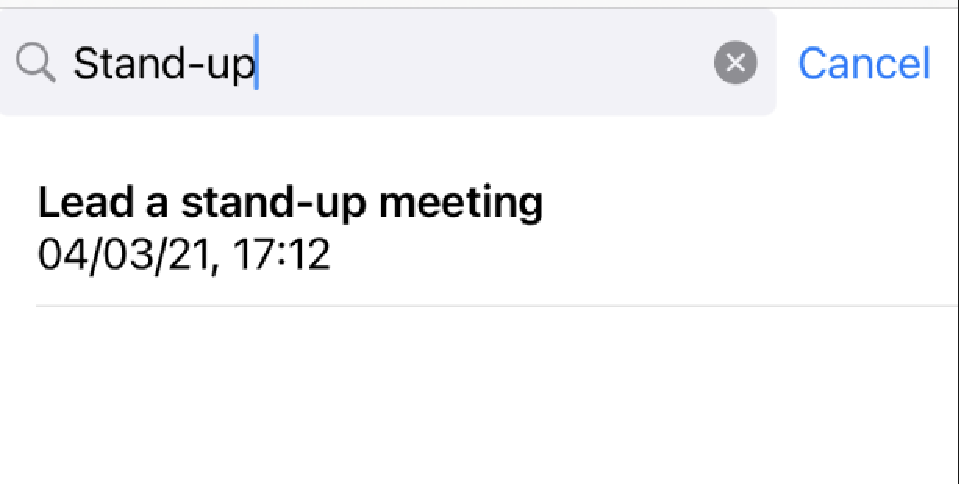
\includegraphics[scale=0.4]{images/SearchFilter.pdf}    
    \caption{This screenshot shows the list filtered after searching for a term in the name of one of the notes.}
    \label{fig:SearchFilter} 
\end{figure}

\subsection{Record an Audio Reflection}

Users are also able to record an audio of themselves discussing a situation or skill. This provided a more convenient option. An AVAudioRecorder object provided the recording capabilities within the app, using the user-built-in microphone and speaker. SwiftUI provides a strict format for allowing audio within an app, this is intended to reduce programming overhead. An AVAudioSession is used to configure the audio session of the app. Each time a recording is started a new audio session is created and set to the category playAndRecord, meaning that a user is able to create a recording and play it back. It ensures that the app will conform to typical iOS behaviours, such as muting audio upon locking the device, or silencing other background audio when a recording is played. 
Users are able to start a recording until they click stop; the recording button can be seen in Appendix \ref{fig:appRecordingsScreen}. AVAudioRecorder will be provided the file name from the user if they had entered it in the name field on the view prior to clicking record. If no file name is given it will set the name of the recording to the date and time of creation.

\subsection{Playback and Delete Recording}

Users are able to playback a recording allowing them to convert this recording into a fully written note, this playback button can be seen in Appendix \ref{fig:appRecordingsScreen}. They can then delete any notes in the same way as a written note via either the edit button or swiping to the left. Edit mode for this can be seen in Appendix \ref{fig:DeleteAudio}.


\subsection{Review Statistics}

Users are able to view the statistics of their notes, seen in Appendix \ref{fig:appStatScreen}. Each skill is presented with the same colour scheme used in the skill descriptions to ensure a cohesive look to the app. Each skill card contains the number of notes they have made on the skill, the average words per entry, and their average emotional response for the skill. Users are also able to view their total number of notes and their average word per note. This was to allow the user to make comparisons between each skill, the length of their reflections, and how they generally view experiences that engage this skill. The average emotion over all skills was not given as a metric, as it was decided it is more useful to review how they feel about a specific skill rather than overall experiences.

\subsection{Visit Useful Links}

The Settings view provides users with links that could potentially assist them in their reflections. One of the links provided takes the user to the University of Glasgow website on graduate attributes, linking this project to the university and how it expects them to develop these skills throughout their education. A link was also given to the University of Glasgow's Moodle page. This was because exporting reflections to Moodle had been considered during the requirements gathering stage, but it had been decided that it was not useful. SwiftUI and iOS development also did not provide a Moodle API to allow users to do this. Instead, a link is now given to users, again linking to the University of Glasgow. These links can be seen in Appendix \ref{fig:appSettingsScreen}.

\subsection{Notifications}

Users are able to turn on notifications through the Settings view. This was implemented using a UNUserNotificationCenter object, which manages all notification related activities. Similarly to enabling recordings, SwiftUI provides a standard structure that allows notifications to be set up and enabled. The UNUserNotificationCenter manages permission requests for GradReflect to send notifications to the user and scheduling when these notifications can occur. In the implemented app, the user is able to click to turn on notifications, setting a notification to launch after 10 seconds, providing enough time to close the app and wait for the incoming notification. This allows notifications to be tested during demonstrations and evaluations. For future deployment, the notifications would launch weekly, as this has been stated as the recommended timescale to regularly reflect \citep{bruno_reflective_2018}. The notification can be seen in Figure \ref{fig:Notification}.

\begin{figure}[H]
    \centering
    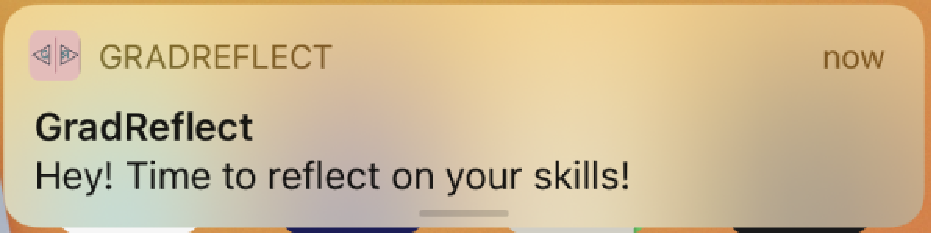
\includegraphics[scale=0.4]{images/Notification.pdf}    
    \caption{This screenshot shows the notification that launches after the user turns on notifications.}
    \label{fig:Notification} 
\end{figure}

\subsection{About GradReflect Page}

Users were also able to navigate to an About GradReflect view through the Settings view, seen in Appendix \ref{fig:AboutApp}. This was a simple description of each aspect of the app and how the app was intended to be used. This section also describes to the user the use of CBT within the app and how this is intended to assist them. The goal of this page is to provide users with further clarifications of how they can use the app to develop their skills and provide greater detailed instructions and support necessary for them to be able to reflect effectively. 


\section{Maintainability}
An important goal for the project was to allow future developers to maintain the project and to add new features, eventually taking this app into deployment through the app store and potentially making a cross-platform version to allow use with any mobile operating system. Steps were taken to ensure that the code and documentation were of high enough quality to allow this. These steps are listed below.

\subsection{Documentation}

\textbf{Code Commentary:} Code commentary was used through the implementation process to ensure that the purpose of code was always clear. Upon completion of the project this commentary was further developed into a narrative throughout the code to show the links between views, functionality, and where data is being passed. This will allow any future developers to quickly understand how the app was made, fix bugs, and add new features.

\textbf{GitHub Wiki:} Throughout the course of the project, the GitHub wiki was kept up to date with weekly progress, meetings and research. The wiki also contained the goals and requirements for the project. This means that anyone reading the wiki is easily able to understand the objectives of the app and the research that went into the design of the questions, the intentions behind reflection, and developing user graduate attributes. This understanding would help any future developers carry through these intentions into their own further development of the app, maintaining the key goals at the core of development. 

\textbf{Developer Readme} A readme for developers is also included in the project. This explains how to set up the project for continued development and how to run the app both on XCode Simulator and on their own iPhone. This is intended to make it easier for any future developers to create new features to the app. 

%==================================================================================================================================
\chapter{Evaluation} \label{evaluation}

This chapter outlines the procedure used in evaluating the mobile app, GradReflect, with the goal of answering the aims stated in Section \ref{IntroAims}, whilst also identifying some potential areas for improvement. These are listed in the future work in Section \ref{Concl_futureWork} due to time constraints, or because they were seen to be out with the scope of the project. 

The results from both the usability experiment and subsequent surveys are presented, with a discussion on how the project meets the requirements and relates to the wider literature of graduate attributes.


% \section{Aims - maybe take this out?} \label{evalAims}

% While the overall aim was to create a mobile app to capture reflections on when and where students have exercised their graduate attributes, \ref{IntroAims} also outlined the extended aims of creating an app that will assist users in making deeper reflections and developing their skills further using CBT. This is, however, a broad aim that would require a long-term experiment that is outwith the scope of this project to definitely answer it. Instead, this aim has been broken down into a series of smaller research areas that will contribute towards answering the larger topic:

% \begin{itemize}
%     \item Is the app easily usable and satisfying for students to make reflections and navigate through, making either written or audio formatted reflections?
%     \item As an extension to the previous aim, can users see themselves using this app again in the long-term? This will give insight into the long-term apps of this project, continued use of this app could result in continued development of these skills and increase the employability of the students.
%     \item Lastly, do students find it helpful and easy to reflect on their experiences? Does an app like this aid their self-analysis? Does each section of the app contribute to this understanding and reflection?
% \end{itemize}

\section{Personal Evaluation}

Before conducting any evaluations with participants, a stage of personal evaluation was carried out. This was to identify any usability problems before any participants were asked to evaluate and use the app. 
 
To gain an insight into how the users would interact with the app, the app was installed onto a personal device and each section of the app was explored similarly to a new user. Following this, an informal heuristic evaluation using Jakob Nielsen’s “Ten Usability Heuristics” was conducted \citep{Nielsen10}. 

\subsection{Results}

From analysis made in relation to the usability heuristics changes were identified that should be made to the app before allowing participants to have access for their evaluations. These changes were as follows:
\begin{itemize}
    \item Addition of a 'Cancel Note' button when creating a note (Heuristic: User control and freedom)
    \item Addition of an 'Edit' button on the notes list view, this was intended to make the app more intuitive for non-apple users who could potentially not be familiar with the typical 'swiping' gesture (Heuristic: Recognition rather than recall).
    \item Changed the position of the 'Edit' button to remain consistent with the position in the notes list view (Heuristic: Consistency and standards).
\end{itemize}


\section{Monitored User Evaluation}

The monitored user evaluation aimed to gain feedback on how usable the interface was from selection of potential end users. After signing consent forms, participants then had the opportunity to interact with the app. This was done using the simulated iPhone, built-in to the XCode IDE, through a video conference where they were given remote control. This method was chosen as it would give the users the chance to get, as much as possible, hands-on experience of the app while lockdown measures precluded face-to-face evaluations. This would be more beneficial than users viewing video demonstrations of the app, as it would give more insight into how a user will interact with the app in a real-world environment. Without carrying out a real-time interaction with the app actual user interaction would be largely unpredictable.

\subsection{User Group Selection}

For this evaluation a total of 8 participants were gathered from a convenience sample of students from various degrees, consisting of both young and mature students. 

The majority of participants were in the age range of 18-24, with this range having 5 participants. There were 3 participants in the 25-34 range. A total of 4 participants identified as female, and 4 participants identified as male. Most students had a strong technical background, with 4 participants currently studying a university level qualification in computing. The remaining 4 participants had never studied a qualification in computing.

Having participants from degrees other than Computing Science allowed for more generalisable results. Having a sample made only out of Computing Science students may give the results an unfair bias as these students are more likely to be quick to understand various interface layouts. Using students from multiple degrees and age ranges, meant that we could give insight into how this app could be useful to any student of any background or experience, as the target demographic for this app is students developing these skills for the workplace.

\subsection{Procedure and Monitoring}

The monitored aspect of this evaluation allowed for a better understanding of how the users interacted with the app, and not just their final results and opinion. Observing the participants allowed any hesitations, difficulties or mistakes made during the use of the app to be noted. Users would perhaps forget these difficulties if only asked to answer a post-use survey. A monitored evaluation also provided the opportunity for the participants to ask any questions, and to use a 'Think Aloud' approach as they were encouraged to voice any of their thought processes or difficulties as they used the app. This allowed any points of interest to be noted by the experimenter alongside the participants’ actions \citep{lewis_task-centered_1994}.

Conducting this study over video conference also meant the evaluations could be recorded, allowing for review of the evaluation to gain further insight into the reactions and comments the participants made. Additionally, remote evaluations would allow participants with experience of any mobile operating system to be included within the survey. This allowed for insight into whether this app would be intuitive for all users, implying that the same or similar designs could be taken to create an app for other platforms. This would benefit any future studies into the use of a mobile app employing CBT techniques to capture graduate attribute reflections. 
 
Participants were given time to familiarise themselves with the app and its controls via their mouse and computer. This was key as using a mobile app through a laptop or desktop is unfamiliar to most users. Allowing for familiarisation prevents the participant evaluating the simulator, rather than on the app itself. 
 
Following this, users were then asked to complete a set list of tasks. These tasks were created to make sure that the participants explored every section of the app and therefore had a holistic view of the app. At the conclusion of this monitored evaluation, users were given another opportunity to voice any opinions of the app.


\subsection{Task Explanation}

The tasks that users were given involved exploring the features of each view of the app. The tasks users were asked to complete can be seen in Section \ref{Appendix-taskList} of the appendix.

\textbf{Home Page} Users started here as this allowed them to familiarise themselves with the graduate attributes they would need for future reflection, as any new user would. 
 
\textbf{Settings Page} Users were asked use each feature within the settings page. Users were asked to follow links to additional information, customise the app, use notifications and read about the general purpose of GradReflect.

\textbf{Notes Page} Users were then asked to create a note based on the skill of teamwork, and given the option of using the '?' buttons should they need to. This tested the users’ ability to be able to reflect easily with the aids and prompts given to them. Users were also asked to review this note and to attempt to create a note with no name. This was to allow users to familiarise themselves with the reviewing process and test error prevention. Finally, in this section users were asked to search for a note or skill. Users were asked to delete a note, testing how intuitive this is.
 
\textbf{Statistics Page} Users were asked to view the statistics based on the note they created. This allowed evaluation on the usefulness of this later in the survey. 

\textbf{Recordings Page} Users were asked to create a recording with and without a name, testing the different naming options allowing for evaluation of recordings in the survey. The participant then had to playback and delete a recording, again testing to see how easily users would be able to do this.

\subsection{Results}

The recorded monitored evaluations with participants were reviewed and any notable difficulties or comments from the participant were transcribed and then grouped together to identify major themes from the tasks. For certain tasks, users encountered no difficulties and made no comments. The most significant themes that were found during the evaluation are presented below. When referring to specific participant responses they are referred to by their ID number to maintain their anonymity.

\textbf{Initial exploration of app}

When participants were given the opportunity to explore the app it was noted that every participant scrolled through some, if not all, of the skill cards. Some participants navigated through every view and component of the app before beginning the tasks. Participant 1 noted that they thought having a section for audio recordings was "cool". Participant 2 voiced that they enjoyed the images that accompanied the skill cards, echoed by participant 8 during their evaluation. Participant 2 also stated that they liked that the statistics page also included the average word count over all notes created. Participant 8 also stated that they thought the app was overall “very cool".

\textbf{Reviewing the descriptions of the skills}

Participants overall appeared to enjoy the descriptions of the skills. Participant 1 stated that there was "good use of examples", the descriptions were not "long-winded", and that the images were useful and enjoyable. Participant 4 also stated that they enjoyed the images. Participant 2 stated that the images helped them to further understand the descriptions of the skill. Finally, participant 6 stated that they liked the "simplicity" of the app descriptions and stated "there's enough information without overwhelming you by having to read a big essay to be able to understand".


\textbf{Following the useful links}

In this task, participants were to follow links from the app to useful pages about graduate attributes, the project GitHub and Glasgow University's Moodle page. This required the participants having to be able to close the app Safari on the mobile simulator and open the GradReflect app again to return. Participants 2, 4, and 5 struggled to be able to do this due to the need to click an alternative 'Home' button that was responsible for closing any app running inside the mobile simulator. However, this is due to the nature of conducting the experiment over a video conference and is a reflection on the simulator rather than the app. Participant 2 also noted that they liked the link to the university Moodle page.

\textbf{Reading the 'About GradReflect' page}

Whilst reading the 'About GradReflect' page participant 6 stated that they liked "the part that said 'notes require a title', as it helps if you can't understand why something isn't working and there's an answer available" and further stated that there was "a lot of good information" on this section of the app. Participant 7 noted that due to the app being on a laptop it "felt weird to have the text all the way up to the sides, but if it was actually on a phone I would like it up to the sides".

\textbf{Turning on and waiting for the notification}

In this task, users only had to wait 10 seconds due to notification being a proof of concept for testing and evaluative purposes. However, again due to this task requiring users to close the app, some participants, including participant 3 and 8, struggled with locating the simulator button to close an app. Participant 2 noted that the ability to have notifications was "cool".

\textbf{Changing the theme of the app}

Overall, participants seemed to enjoy this feature and its customisability. Participant 2 and 8 specifically stated that they enjoyed having this feature.


\textbf{Creating and saving a note}

In this task, participants frequently made use of the question help '?' buttons, with 7 out of 8 participants using them at least once. Participant 3 needed clarification of where to enter their notes. Participant 4 initially attempted to create a note by clicking the 'Edit' button on the notes list view, but quickly realised where the 'Add note' button was located and went on to use that instead. Participant 5 struggled with scrolling on the page due to having to hold down with their cursor, however, this was due to it being a virtual phone. Participant 6, when using the emotion slider, initially attempted to click on the scale where they wanted to adjust the slider to, when this did not work, they knew to drag the scale to their desired position. Participant 7 struggled to see where to select the skill type but after asking, they were able to choose the skill subsequently.

\textbf{Reviewing a note}

Participants did not struggle to open the note after creation. However, participant 1 stated that they wished they were able to scroll with their mouse instead of holding down their cursor to push the screen up. This is due to conducting the evaluation virtually as the simulated phone requires the mouse to act as a finger would on the screen. Participant 6 noted they had not answered the questions the way they had intended as they had not read the questions properly, and in the future, they would know how to answer them better.

\textbf{Reviewing the statistics}

During the review of their notes, participant 2 stated that they enjoyed the statistics as they are helpful when evaluating yourself and whether you are good and bad at something. They stated this was especially the case with the emotion and how much you have written, getting an idea of how much you have written and how much detail helps to get an idea of your own thoughts and what to do moving forward.


\textbf{Deleting a note}
 
In this task, some users struggled with understanding how to delete a note. When asked to do this, participants 1, 3, 5, 6, and 8 attempted to delete the notes by opening the reviewing view of a note and scrolling to the bottom. However, after realising there was no button to delete a note there, they found the 'Edit' button and saw that this would let them delete notes. 

\textbf{Creating a named recording}

During this section, participant 1 at first attempted to record a note by holding down on the record button instead of tapping it. However, after seeing this did not create a note and just started the recording after releasing the button, the participant tried again. However, the note did not save. Later attempts to recreate this issue resulted in no errors, meaning this issue was transient. Once they then renamed and created a recording, they were able to create an audio note. No other issues were encountered from participants with creating a recording.

\textbf{Playback a recording}

During this task, further issues were encountered due to the necessity of conducting this evaluation over a video conference. When creating a recording the simulated phone was connected to the experimenter microphone and therefore only faintly picked up what the participants were saying. The participants were then not able to hear back any audio from the simulator as the video conference was not sharing any audio from the experimenter’s computer device. However, the experimenter was able to hear back the recordings quietly, ensuring that the participant knew that their recording had worked. No participants had any issues carrying out the actual task.


\textbf{Comments given by participants at the end of the tasks}

At the end of the tasks, participants were given the opportunity to voice any comments about their experience. Participant 2 stated they found it easy to use, especially as it used familiar iOS practices. Participant 4 noted that the app was easy to use and was intuitive and laid out well, as well as being user friendly. They also stated they would use it as a space to reflect about what work they are doing, to think over things at the end of each day. Participant 5 said the app was seamless, worked really well, and was straightforward for the user. Participant 6 stated it was a very good app as it was nice and easy to use, and they could navigate easily and there were clear labels. They went on to say they liked the helper buttons as they gave something to work with in terms of answering the question. Participant 7 said that when deleting any notes or recordings they thought iOS users would swipe rather than click 'edit', however, this was an option that was also available. Participant 8 stated that they liked it and thought it was easy to navigate. They also stated the first time using an app is difficult, especially virtually, but if they had the app they would continue using it as it did seem really simple.

\subsection{Discussion of Results}

The monitored evaluation highlighted several areas where the app had met the aims of the project stated in Section \ref{IntroAims}.

\textbf{Creating an app to capture reflections on graduate attributes:} Every participant was able to make a note about their experiences and reflections on a time they used the example skill teamwork.

\textbf{Allow users to create a note via written or audio form:} All users were able to make a note with both written and audio formats. This shows that for future use of this app, users would be able to make a choice about which method is the most convenient for them to reflect. Having this ability to make reflecting easier could encourage more users to reflect. The only issue encountered during audio recordings was due to the virtual nature of the evaluation. Recordings were not audible to the participant which did not allow them to completely engage with and comment on the process.
 
\textbf{Remind users when they should reflect:} All users were able to turn on the notifications that sent out a reminder to the participant 10 seconds after clicking, with some participants specifically stating they enjoyed this feature. 

\textbf{Create a usable app:} From the results of the monitored evaluation, it can be seen that the majority of users faced no issues when using the app, and overall enjoyed their experience. Participants noted several areas that they particularly enjoyed. The minimalist design of the skill cards made clear to the users what was important when reflecting using the app, with the accompanying images helping to deepen understanding. This minimalism meets the usability heuristic of aesthetic and minimalist design. In the settings view users enjoyed the customisability the app provided through the ability to change the theme, also noting that the app provided good documentation within it to help with any issues users might encounter, demonstrating the heuristic of ‘flexibility and ease of use’, and the heuristic ‘help and documentation’. Within the concluding statements of the evaluation, several participants stated the app as being intuitive and user-friendly. During the survey, participants made statements about how they would use the app in the future, for example, when they would use the statistics page, how they would get more familiar to the app the more they used it, and how in the future they felt they would answer the questions with better responses. This demonstrates that the participants were showing an interest in how this app could be useful to them in the future.

\textbf{Aid reflection:} During this evaluation, the app's ability to assist in reflection was highlighted as the users created their first note. The help buttons were used by the majority of participants. They were seen to ground the user in what to reflect on and after users had read these, they were able to quickly make a reflection based on this. The prompts followed the CBT approach, which from Section \ref{ExploratoryStudy} has been shown to encourage deeper reflections. Users were also assisted through the descriptions given from the skill cards. Participants stated that these descriptions gave them a better understanding of what these skills are, and therefore they should be able to make better reflections on these skills as they become more aware of what they are and when they use them.

\subsection{Future Work Identified by Observing Participants}

The following potential changes were identified:
\begin{itemize}
    \item Allow users to delete a note from within a note review view.
    \item The emotion slider could allow users to click where they want the slider to go, as well as being able to drag it.
    \item Make the button to delete notes clearer to the users, make it red with a 'delete notes' label next to it. Include in the app description that users are able to both click the edit button, and swipe in the typical iOS app gesture.
\end{itemize}

All of these changes make sense to be added to the app and can be seen as future work.

\subsection{Limitations}

While the design of the evaluation determined whether the project aims had been met, there are a number of ways in which the study could be improved.

Although this app is intended to be used on student's personal devices, the decision was taken to run these experiments in a controlled setting over a Zoom conference. This was due to this being an iOS app, meaning it would require an Apple developer license to be able to widely distribute this app through the Apple App Store. To test and install this app on their own device, users would need to be able to connect their phone to the experimenter's computer. However, this project was conducted during the COVID-19 pandemic, meaning it would not be safe to meet with experiment participants for testing purposes. 

Conducting this experiment virtually allowed testing of the app during the COVID-19 pandemic, however, this may have affected the behaviour exhibited by participants. For example, users were not able to use the controls of the phone as easily and at times struggled, instead having to opt for a 'Home' button outside of the simulator to be able to close the app instead of the typical 'swiping' from the base of the phone to close an app. This, at times, created frustration for the participants as they attempted to use the option that they would on a physical phone. This environment also caused issues when a participant was not able to access the additional 'Home' button of the simulator as Zoom had a 'Remote control' taskbar display on top of this button, causing confusion and delay as the participant realised they needed to remove this taskbar on their device to view the 'Home' button. Therefore, further studies should be conducted that allow a participant to be able to install on their own device or use an experimental physical device to evaluate the app. This would ensure that the behaviour observed is representative of the behaviour that would be exhibited in-person.

Additionally, the participants came from a convenience sample of friends and family members. Therefore, this could have also impacted the behaviours exhibited by the participants, as a result of social-desirability bias \citep{lavrakas_social_2008}. Further studies should take care to conduct their experiment using a more representative sample of unknown participants, to ensure the results are representative.

\section{Post-study Survey}

Following the completion of the monitored evaluation, the same selected participants were then asked to fill in a post-study survey. 

\subsection{Procedure}

The post-study survey had two sections.

The first section of the survey took inspiration from both Nielsen’s approach of conducting a heuristic evaluation utilising his approach of identifying and evaluating ten usability areas, and Brooke's System Usability Scale (SUS) \citep{Nielsen10, affairs_system_2013}. Nielsen's usability heuristics typically are used by usability experts. However, they were used in this evaluation due to usability being a key aim of the project, as these heuristics detail important aspects that provide a key indication of how usable a system is. To make sure these points were able to be evaluated easily by both the computing-based participants and non-computing-based participants, the questions were framed in plain, non-technical English and explained clearly. Participants would respond to these questions via a series of statements based on whether they agree or disagree on the usability, as dictated by SUS. These ranged from "Strongly disagree' to 'Strongly agree'. This allowed identification of any issues or improvements that had not previously been identified. 

In the second section of this survey questions related to the features of the app were posed. This section also took inspiration from the questions used in the SUS evaluation. This was to establish users' general feeling towards the app by asking how they found using different features of the app. The survey asked if they found it quick to make a note, if they would be likely to use the app again, and if there were enough aids to help them reflect. The specific features asked about were the audio recordings and the statistics sections. These were sections that were added to the requirements in a later iteration of the design, and therefore insight into participants' reaction to these features would demonstrate whether they were valuable. 

Participants were asked to fill in a survey, these questions can be seen in Appendix \ref{Appendix-EvalSurveyQuestions}.


\subsection{Results and Discussion}

\textbf{Survey Part 1}
 
The response to each of the usability heuristics was gathered and put into individual graphs for each heuristic, these can be seen in Appendix \ref{Appendix-surveyP1-individualHeuristicGraphs}, and then processed further by taking the average response to each usability heuristic. This graph can be seen in Figure \ref{fig: UserStudyGraph}

\begin{figure}[H]
    \begin{centering}
    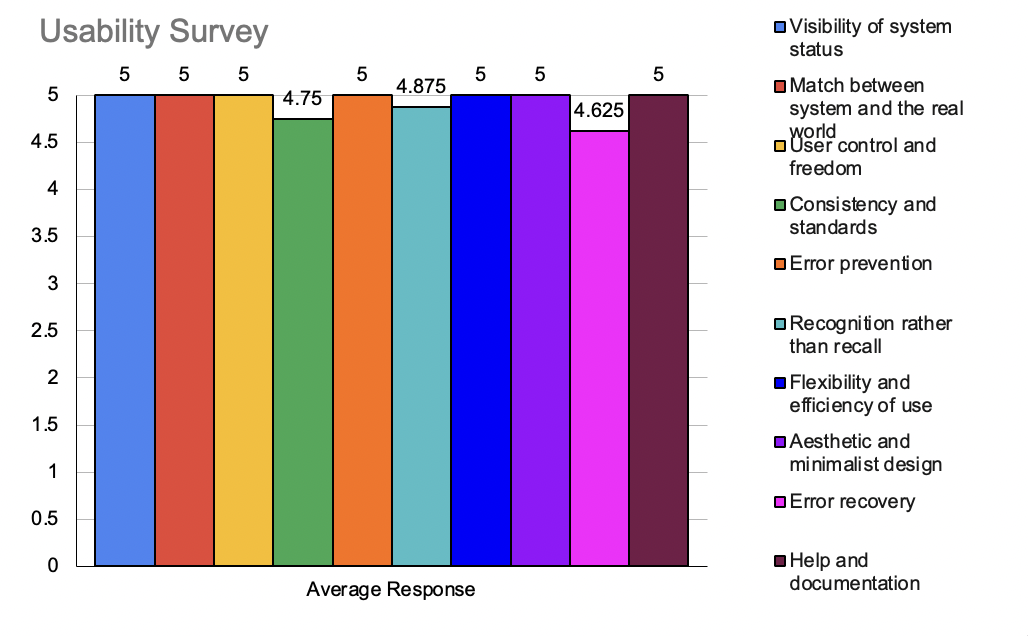
\includegraphics[scale=0.75]{images/UserStudyGraph.png}
    \caption{This graph shows the average response of participants to each of Neilson's 10 Usability Heuristics from the post-study survey carried out as part of the evaluation.}
    \label{fig: UserStudyGraph}
    \end{centering}
\end{figure}
 
Most participants strongly agreed that the system was usable and satisfying. For 8 out of the 10 usability heuristics, participants all strongly agreed that the app entirely met these standards. However, 3 of these heuristics, consistency and standards, recognitions rather than recall and error prevention, did not entirely meet these standards but scored very highly.
 
From this first section of the survey, participants were also able to explain their motivation behind their scorings. These open-ended answers were all themed around the heuristic question they followed. Therefore, two major themes were used to categorise responses. These themes were ways in which the app was easy to use, and any issues users had with the app.

\textbf{Ease of Use:} When giving comments on their answers many participants stated explicitly how they thought the app was easy to use, intuitive and clearly laid out. One participant stated, "Simple to understand for a technophobe like me". Other participants mentioned that the navigation was clear to follow, with buttons being placed logically so they were easy to find, and the app used features that were very familiar to typical iOS design and other similar apps. Error messages were also stated to be easily identifiable and understandable, with users noting that it was made clear what the issues were and how to solve them. Participants also noted that they appreciated the extra help icons as they gave more direction to the users on how they should be answering the questions. This shows that generally users did not find using the app difficult, making for an enjoyable experience.

\textbf{Issues users had with the app:} For the areas where users did not strongly agree with the heuristic they were able to give explanations for their answer in the comments. The heuristic for consistency was given 2 agree scores. One participant stated "I am an android user" as their explanation. This could be due to the app mostly following native to iOS design practices and not being familiar for someone who has experience in only android phones. This could make it more difficult for a user. The other participant stated as their comment \begin{quotation}"The app used a consistent colour scheme throughout and consistent and intuitive navigation options between and within the apps pages and sections. The settings page was also made to look similar to the operating systems main settings page. This consistency with other systems made it easy to understand its purpose."\end{quotation} This does not give a clear indication of why this participant did not score this heuristic as highly as the other participants.

Recognition rather than recall also did not score as highly. One user stated \begin{quotation}"This was easy to understand throughout. On the create note page I scrolled down to understand the full extent of the form and what was required of creating a note before completing it."\end{quotation} This shows that this user was unsure of what would be necessary for them to reflect before they had looked at the entirety of note creation view, meaning that on first viewing of this page the user could potentially not be using this note creation to its full potential. 

Another participant scored error prevention as neutral, however, this was not stated to be a negative review of the app as the participant explained "I encountered no errors". This scoring could show that the user did not feel the need to rate this attribute positively or negatively as they had not witnessed any errors within the app.

\textbf{Survey part 2}
 
Following this section of the survey, users then had to answer questions relating to their preferences and experience with the app in general. 

The survey asked about specific features of the app and targeted the aims of the project to find insight into whether the participants felt these were met.
 
\textbf{Creating an app to capture reflections on graduate attributes:} The first question asked the users how easy they found reflection. 7 out of 8 participants rated the app as very easy to reflect with, with 1 participant rating easy. This shows that for the majority of people, this app was overall very useful for users to reflect and provided enough assistance and prompts for the users to reflect on their graduate attributes without any issues. However, there is still room for improvement to make this process more seamless for every user.

\textbf{Allow users to create a note via written or audio form:} All participants stated that they felt the ability to create audio recording was useful, with several participants stating that they would be useful for quick and convenient reflections as they are less formal. One user stated that "The recording section, in particular, took very little time and effort to add to and often saying how you are feeling can make it more memorable, enhancing its usefulness". This shows that the addition of the audio recording feature assists users in being able to reflect via more than one format, and that there is value in being able to think out loud about graduate attributes. This ease of reflection could encourage users in the future to carry out more casual and frequent reflection. 

\textbf{Create a usable app:} When asked if users were able to quickly create a note, all participants voted yes. Users stated that it was intuitively designed and easy to simply fill in the boxes. One user stated that the questions and prompts helped to break down their thoughts easily. This shows that the design of the app and the use of the CBT line of questioning and prompts helps the user to quickly be able to make notes based on meaningful reflections.

When asked if users would continue to use this app, all participants voted yes. In the comments for this question many participants noted the ways they felt an app like this would be useful for them in the future. Two participants noted that this app could be useful for future employment by helping them list the skills they have used that would be crucial to the workplace and help to develop their CV, with another participant also stating that it would help them to "see the skills I have developed outside of the basics of my degree focus". This shows that participants have identified the key uses for this app and how reflecting on and developing these skills is crucial to assist them in their future workplace. Another participant also noted other ways that this app could be useful stating "Reflection on what you are able to do and how you feel can be helpful for mental health and also inspire you in what you are currently doing", suggesting the app could be used in the future for further benefits than just employability.
 
The majority of users also felt that the statistics page was useful, with only 1 participant expressing they did not enjoy it, stating "Stats aren't my strong point". Participants found this would assist in helping them focus on what skills they need to develop, with one participant noting that it could be encouraging to see what skills have already been developed. This further extends the use cases of the app, allowing them to reflect more efficiently as they would be able to see the areas that are weaker. 

\textbf{Aid reflection:} When asked if participants felt there was enough assistance to aid reflection, all 8 participants voted yes. Participants specifically stated that the helper buttons were very useful, and they appreciated the additional information to prompt their reflections, as well as showing how the app was meant to be used. One participant specifically stated, "I found the prompts helped me to think in a deeper way about the situation I was describing, it gave me time to think about my emotions/reactions." This shows that the app meets the needs of users to help them reflect in a more meaningful way. This reflection would be useful in the future for users to develop their graduate skills further.


\subsection{Future Work Identified by Participants}
The following potential changes were identified:
\begin{itemize}
    \item In the future, this app could be made cross-platform, meaning it require using less iOS design to make it suitable for a user experienced with any operating system. Additionally, an Android version of this app could be made separately to also fit the needs of those specific users. 
    \item In the future, more descriptions of the questions users will have to answer could be added, and the depth of reflection needed from them could be made more clear in the About GradReflect section. Allowing users to preview what is expected of them before they begin to reflect helps them be more prepared and leads to better reflections.
    \item Filtering the notes by clicking on one of the skill categories on the skill cards.
    \item Ability to set goals for number of reflections on a skill and receiving milestone achievements when these are met.

\end{itemize}

\subsection{Limitations}
One major limitation of this evaluation was that it could not have been conducted in person due to the COVID-19 pandemic. Future work would be recommended to conduct semi-structured interviews with participants, as this would allow the interviewer to enquire further and follow-up on the responses that the participants give. This would  gain more insight into what the participants think about their experience with the app.

\section{Requirement Validation}

The final stage of evaluation was to determine if the functional and non-functional requirements, outlined in Section \ref{analysis/reqs}, had been successfully met. 

\subsection{Verification of Functional Requirements}

The functional requirements were evidenced by performance in the user monitored tests, as described above. From these evaluation tasks it is clear to see that all of the functional requirements listed in Section \ref{analysis/reqs} are met by the app. 

% \textbf{Functional requirements}
% \begin{itemize}
%     \item \textbf{MH} Users must be able to capture a reflection of how and when they have exercised and developed their graduate skills, this can be in either written OR audio form.
%     \item \textbf{MH} Users must be able to delete a reflection created, as well as being able to review it at a later date, however users should not be able to update or edit a note after it's creation. 
%     \item \textbf{MH} Users must be able to turn on notifications.

%     \item \textbf{SH} Users should be able to select a skill from a pre-defined list to avoid mistakes and allow for future potential filtering.
%     \item \textbf{SH} When creating a written note, there should be help buttons that explain to the user how they should answer each questions and provide an example, this will give them clear instructions to allow effective reflection.
%     \item \textbf{SH} Users should be able to give their note a title to allow for clear representation of what a note contains, and allow for future potential searching or filtering.
%     \item \textbf{SH*} Users should be able to create a reflection in BOTH written and audio form. This will allow both structured reflections and freeform spoken reflections for convenience. 
%     \item \textbf{SH} The app should contain a description of each of the skills that users are expected to develop and reflect on during the use of the app. 
%     \item \textbf{SH*} Users should be able to search for the name of a note or a skill category to filter the notes in the list by skill.
%     \item \textbf{SH} The app should have a Settings page to view information about the app.
%     \item \textbf{SH} GradReflect should have an About Page within the settings that tells the user how to use the app correctly to make reflections, giving further clear instructions to the user. 
%     \item \textbf{SH*} Users should be able to view statistics based on the reflections written into the app.
    
%     \item \textbf{CH} The app could implement Cognitive Behavioural Therapy techniques to aid the reflection and provide users with a suitable framework to support them and provide clear instructions on how to reflect. 
%     \item \textbf{CH*} Users could have the ability to customise their experience of GradReflect and have the ability to switch between dark and light themed interface.
%     \item \textbf{CH} GradReflect could have links in the Settings page that take users to useful pages related to the app and graduate attributes to provide further insight and education on graduate attributes.
    
%     \item \textbf{WH} It was decided that users will not be able to upload reflections onto Moodle as this is not within the scope and does not provide enough benefit to users in completing the aims discussed in Section \ref{IntroAims}.
% \end{itemize}

\subsection{Verification of Non-functional Requirements}

\textbf{Intuitive and easy to use:} Participants gave clear indication that the app was easy to use, with several noting they felt that the design was clear and understandable. The usability study conducted showed the app scored very highly, with only three of the heuristics scoring less than the maximum in the feedback. 

\textbf{Help to create meaningful reflections:} 87.5\% of participants stated it was very easy to reflect, with 12.5\% stating it was easy to reflect, suggesting the app provides enough support to users to reflect. 

When asked if there was enough assistance to support their reflection, 100\% of participants stated yes. When commenting on their answer they stated they felt encouraged, that they were able to think deeper about a situation, it gave them that time to think about their emotions and reactions, and that generally they felt like the assisting reflective features were beneficial. However, during the tasks where users had to reflect using the app, users did not deeply reflect. This is possibly due to it being a monitored evaluation and users did not want to spend a lot of time reflecting whilst being monitored, and instead wanted to carry on with the rest of the tasks.

\textbf{Quick reflections:} 100\% of participants voted that they were able to make quick reflections, stating it was easy and intuitive, and the recordings especially allowed for a fast, convenient way to reflect.

\textbf{Encourage continued use:} Participants were asked if they would continue to use this app and 100\% stated yes. They stated this app could be beneficial for mental health, inspiring for current work, and useful when collecting their skills for future employment. 

\textbf{Useful/valuable features:} 100\% of participants thought the recordings were useful, stating this feature adds another dimension, increases memorability, and provides a more convenient method. 87.5\% of participants felt the statistics were useful, going on to comment that they would be encouraging, and help to focus where they need further development.


\section{UI Tests}

In the future the app would require extensive UI and Unit testing to be released for general use by the public. However, due to the aims of the project, only one UI test was created to give a proof of concept. The UI feature that has been tested is the users' ability to create and save a written note, as this is the basic necessary requirement for the app to run functionally. This UI test passes when run, ensuring users will be able to capture a reflection on their graduate attribute.

\section{Summary of results}

TO BE ADDED: SUMMARISE RESULTS


%==================================================================================================================================
\chapter{Conclusion}  

\section{Summary}

Graduate attributes are the abilities developed by students during their time in university that increase their employability, allowing them to integrate better into the workplace and create a better environment within teams. However, these have been found to be lacking in graduates entering the workplace. This project looked at building an iOS mobile app to capture and encourage reflections on graduate attributes from students in order to facilitate their development.

A study with 10 participants was conducted to determine whether students were familiar with graduate attributes and how comfortable they are with reflection. This study found that the majority of the students questioned had not heard the term graduate attribute before but knew the importance of these skills in the workplace and are keen to develop them.

Research was conducted into finding a novel way to encourage reflections through the use of Cognitive Behavioural Therapy (CBT), exploring how the use of this app, with the integration of CBT could increase the levels of reflection within students. 

An exploratory study using A/B tests was carried out to answer the question: Does CBT benefit reflection by students on their graduate skills? These tests found that students were able to reach higher levels of reflection more frequently than with non-guiding job interview style questions. This gave an indication that the CBT framework has the potential to assist in students’ development of these skills, as deeper and more meaningful reflection will benefit students in their awareness of these skills.

The app created, GradReflect, allows users to capture their reflection in either written or audio form. Users were given the option of both written and audio format to allow them the opportunity to choose whether they wanted to reflect in depth, or the convenience of creating free-form audio recording. It provides a framework using CBT techniques to encourage users to reach all stages of reflection and provide the necessary support and instructions to allow them to reflect effectively. The app gives the user detailed descriptions of each skill they are expected to develop alongside descriptions, how the app is intended to be used, and how to answer the questions. This makes it clear to the user what is expected of them when using this app and, again, gives them clear instructions to allow them to reflect in a beneficial way. GradReflect also gives users insight into their own reflections, providing statistics based on their written notes. It details for users how many notes have been written, their average lengths overall and for each skill, as well as their average emotional responses to skills. This is intended to focus users on the skills that require further development and reflection. The app also provides notifications to encourage the user to reflect regularly; however, for testing purposes these notifications launch 10 seconds after turning on.

GradReflect was evaluated using monitored and survey-based user evaluations. It was found that GradReflect was easy to use, assisted users’ reflection, and that they would continue to use this app in the future. Some participants stated the various ways they would use the app and how it could benefit them. From these results it was clear that an app such as this has the potential to be greatly beneficial for students in developing their graduate skills.

\section{Future Work} \label{Concl_futureWork}

From the research, implementation and evaluation, there are a number of avenues for future exploration of this topic, as well as changes that could have been made to improve the app. 

The exploratory study conducted at the beginning of the project could be extended into a full experiment where participants answer reflective questions using the CBT framework for an extended period of time. Comparisons between the level of graduate skills before and after the experiment could be used to determine the long-term effects that this proposed method of reflection could have on students. 

The evaluations needed to be conducted in a controlled environment over video conferencing, and so it is possible that some of the participants’ behaviours were not representative of how they would interact with the app if it was actually deployed onto their device. Due to this limitation, a reasonable next step would be to deploy the app and examine how users would interact in person. It could then also be examined where users’ skills improve if given access to this app over an extended period of time.

During these evaluations, users presented several ways they would want to see the app itself improved. As well as these improvements from users, there were potential improvements identified personally.

\begin{itemize}
    \item Allow users to delete a note from within a note review view.
    \item The emotion slider could allow users to click where they want the slider to go, as well as being able to drag.
    \item Make the button to delete notes clearer to the users, make it red with a 'delete notes' label next to it, include in the app description that users are able to both click the edit button, and swipe in the typical gesture iOS apps are able to do.
    \item Filtering the notes by clicking on one of the skill categories on the skill cards.
    \item Ability to set goals for number of reflections on a skill and receiving milestone achievements when these are met.
    \item A tab bar could be used to navigate through the app instead of a home page directing to each section.
\end{itemize}

If the app were to be deployed to iOS users with an Apple Developer License, further developments would need to be made such as the extension of notifications to launch weekly, and further UI and unit testing to be developed. 

\section{Reflection}

Overall, this project has taught me a great deal in terms of individually organising and carrying out a large-scale piece of work. It was a useful learning opportunity, particularly in learning a new language and framework and beginning to use it quickly. The ability to learn a new language and frameworks and apply these in a solo project has greatly improved my confidence and technical skills. It has also highlighted the importance of good project management when working under time constraints. 

The research into different methodologies to encourage reflection and the benefits reflection can have on a student or person, were particularly insightful and these practices will be taken into my future projects and with me into the workplace. Through this project, I feel I have personally developed the key graduate attributes that have been discussed in this paper.

%==================================================================================================================================
%
% 
%==================================================================================================================================
%  APPENDICES  

\begin{appendices}

\chapter{Appendices}

\section{GitHub}\label{AppendixGitHub}

GradReflect Project GitHub Link

\url{https://github.com/gmtmcd/Level-4-Individual-Project}

%==================================================================================================================================
%

\section{Ethics checklists}

\subsection{Graduate attribute survey}

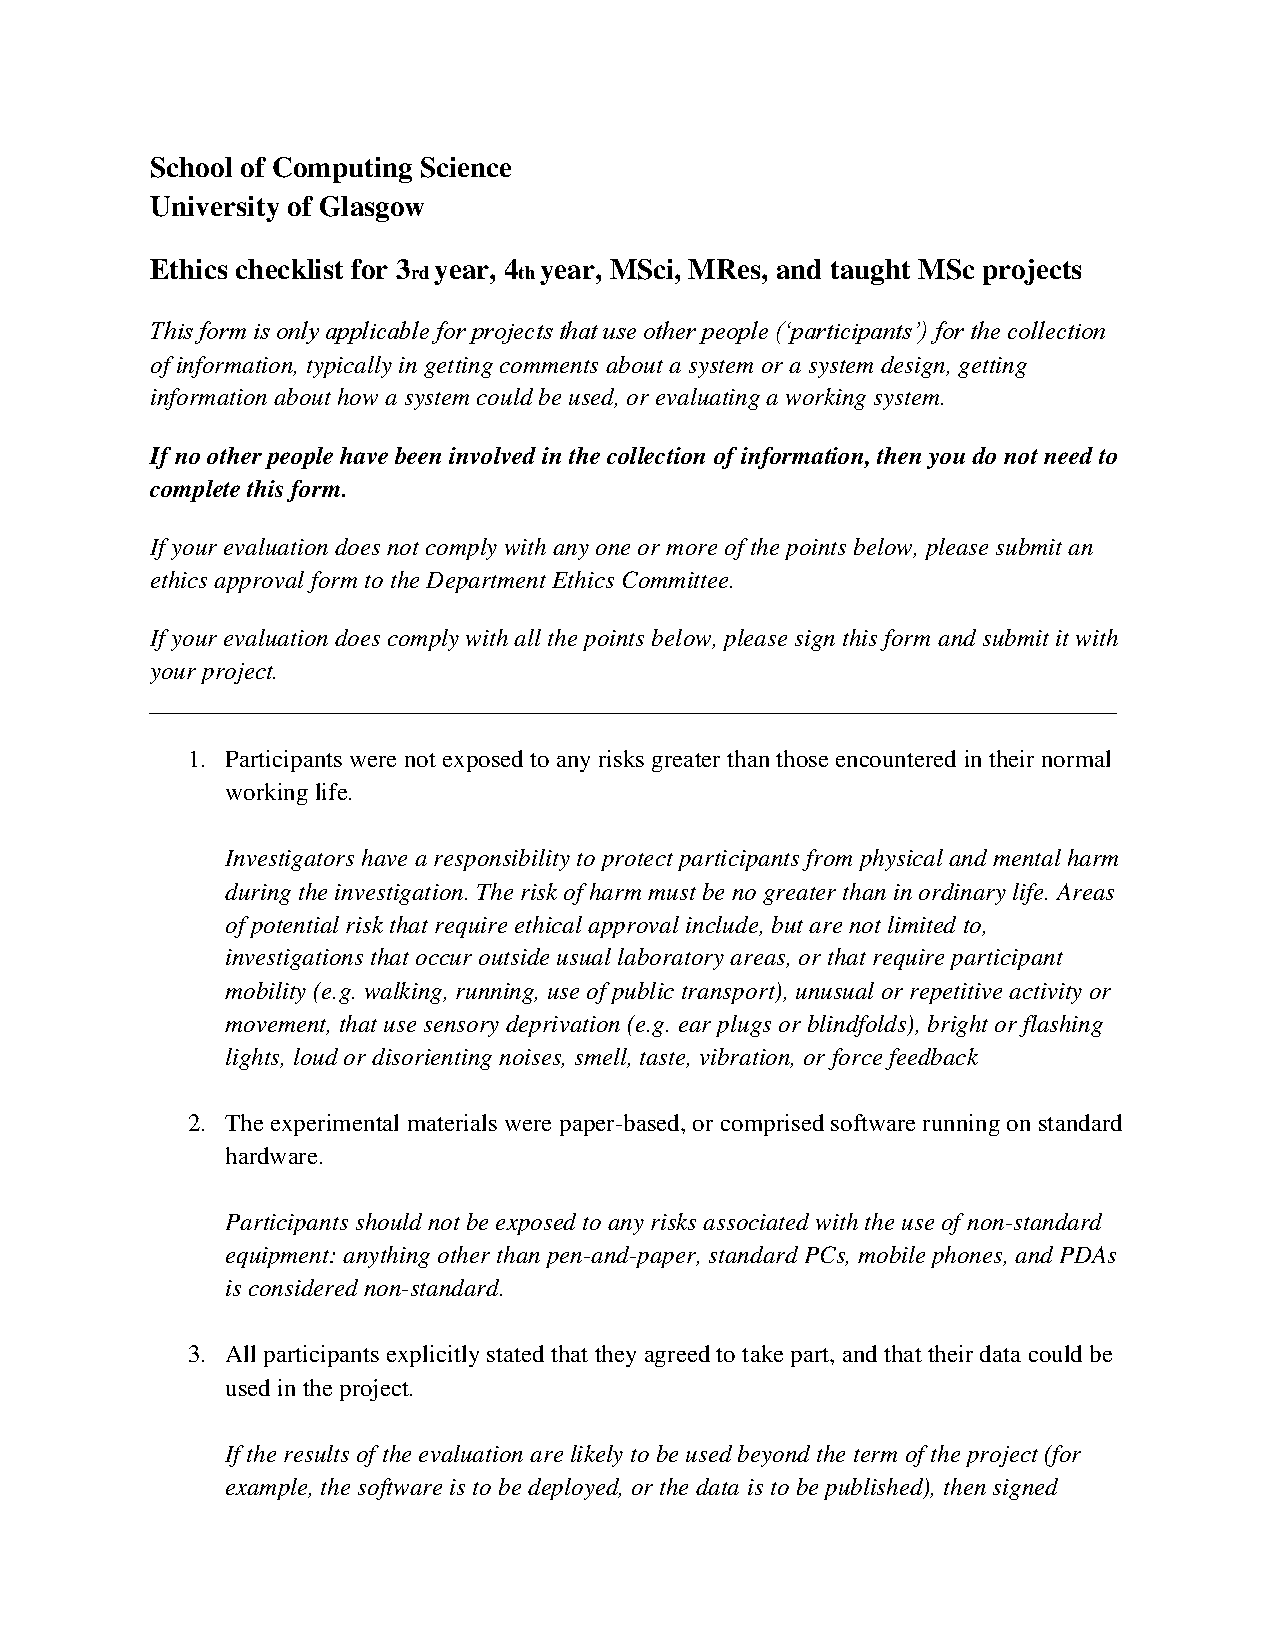
\includepdf[pages=-,pagecommand={},width=\textwidth]{images/EthicsChecklist-GeneralSurvey.pdf}

\subsection{AB tests}

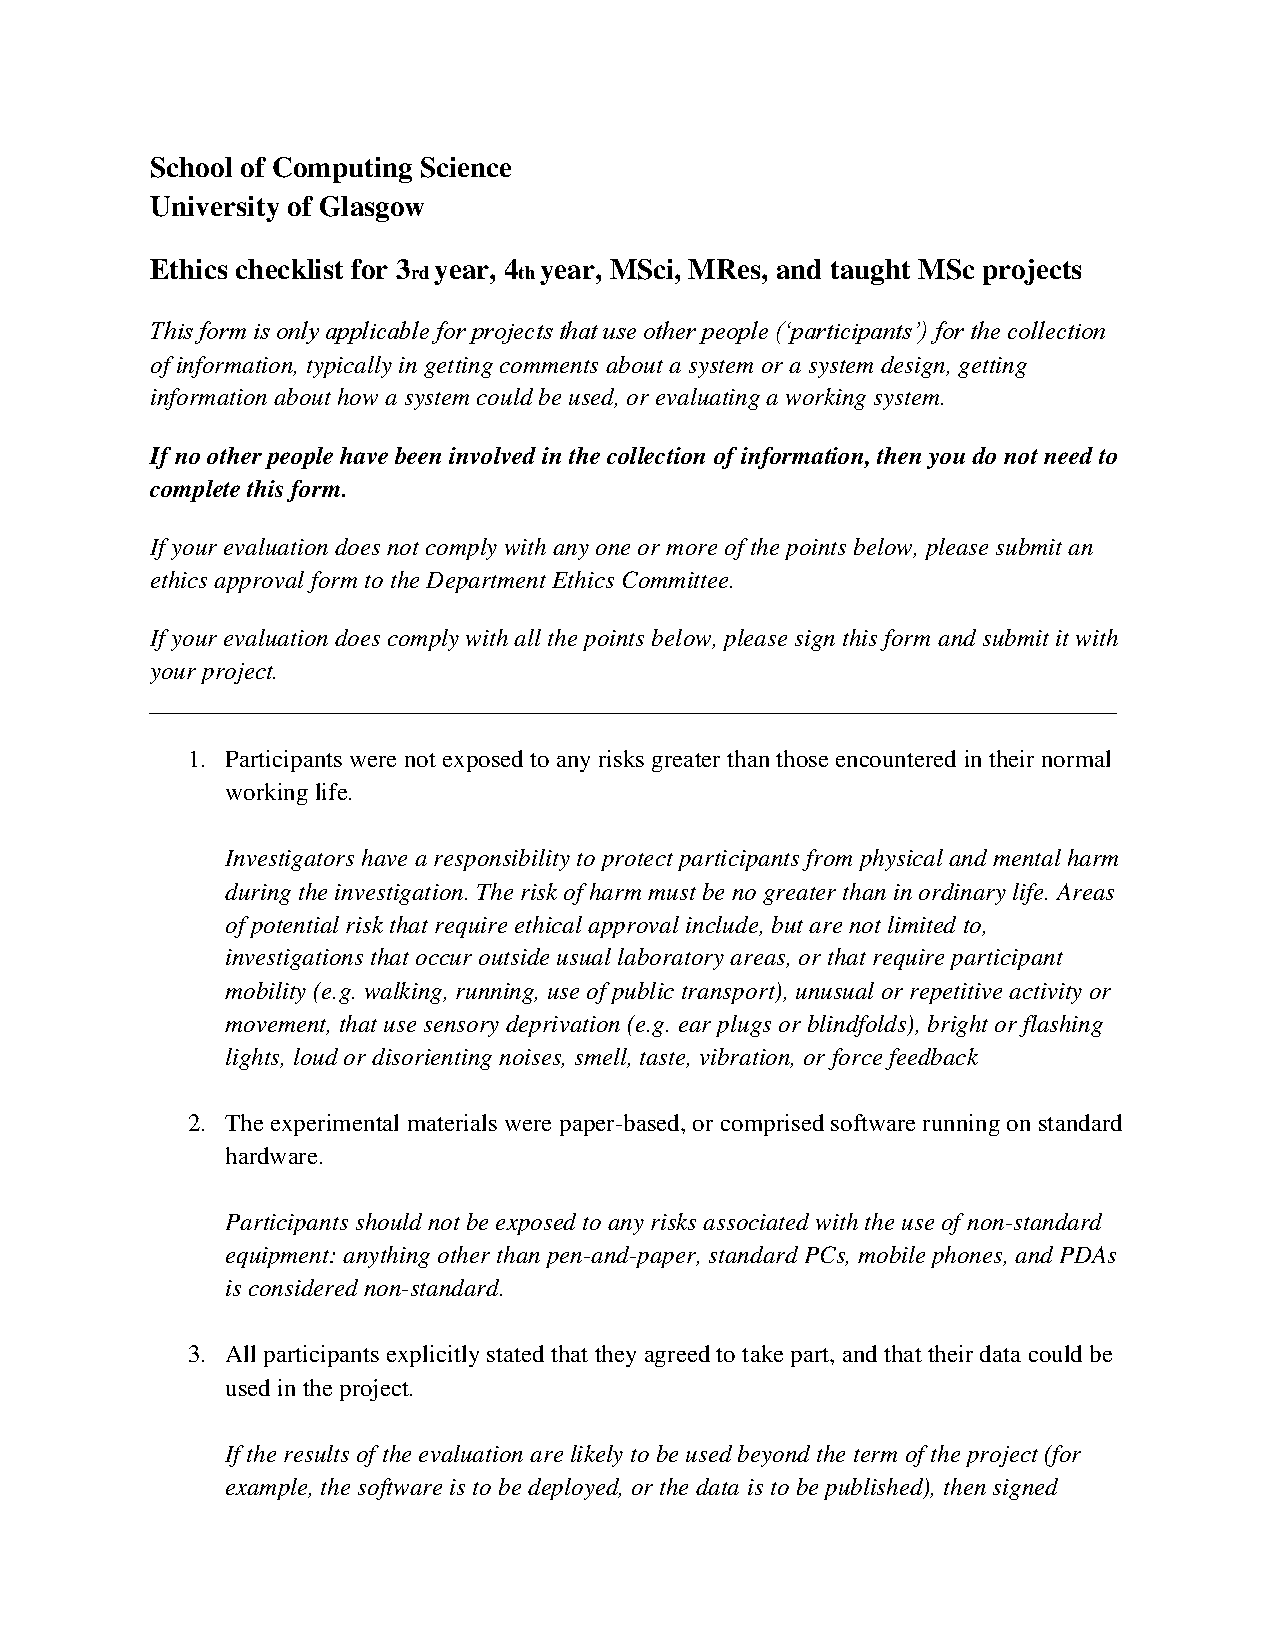
\includepdf[pages=-,pagecommand={},width=\textwidth]{images/EthicsChecklist-ABTests.pdf}

\subsection{User evaluations}

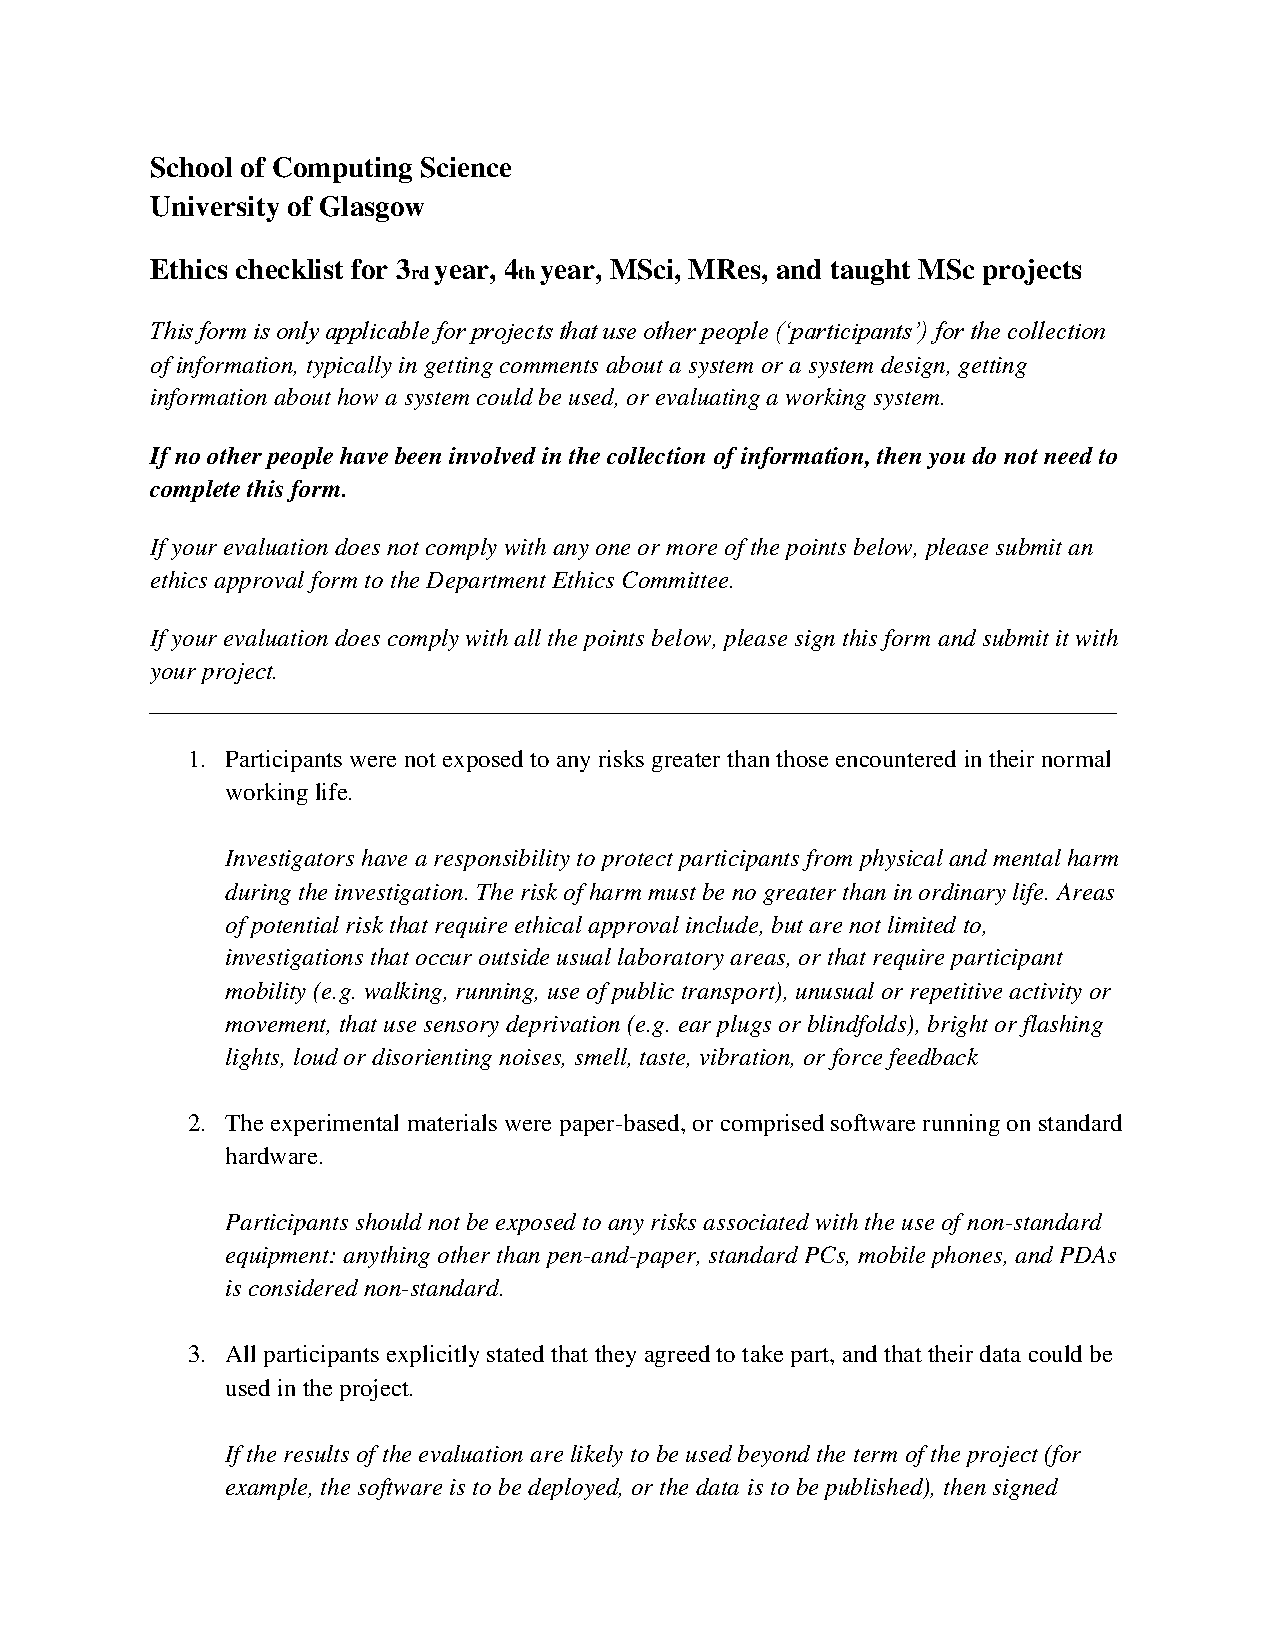
\includepdf[pages=-,pagecommand={},width=\textwidth]{images/EthicsChecklist-UserEvals.pdf}

%==================================================================================================================================
%

\section{Graduate Attribute General Knowledge Survey} \label{Appendix-gradAttributeSurvey}

\subsection{Intro Script}

SCHOOL OF COMPUTING SCIENCE - UNIVERSITY OF GLASGOW

The aim of this experiment is to gain an understanding of students' knowledge of graduate skills and how much these skills are currently integrated into their lives. 

We cannot get an understanding of this without participation from the students who would give an indication of this knowledge base. 

You should answer the questions honestly, giving any extra comments where they feel appropriate.

The answers will be collected and analysed. Please ask questions if you need to, I will be available during and after the survey by email.

Please remember that this is to evaluate the general understanding and development of these skills within students, and is in no way an evaluation on you, the participant.

You are able to withdraw from the survey at any time.

Below is a question asking for your consent to participate in this survey requiring you to select yes to continue, however if you do not consent, just close the survey at this point.

Please remember questions can be asked at any time.

Thank you.

\subsection{Questions}

\begin{enumerate}
    \item Have you heard of the term "graduate attributes" before?
    \item If yes, can you name some?

    \textit{Following explanation of skills is given: "Graduate attributes, sometimes referred to as 'soft skills', are skills learned during someone's time at university, that aren't necessarily a direct result of the courses they are doing. These can involve, but are not limited to:
    - Communication
    - Critical thinking
    - Adaptability
    - Teamwork
    - Self-efficacy
    - Application of knowledge
    - Ethics
    - Professionalism 
    These skills are developed primarily through real-world experiences and reflection."}
    \item Has the importance of these skills in the workplace been explained to you?
    \item Do you have any further comments on the above question?
    \item Would you be interested in learning and developing these skills? 
    \item Do you have any further comments on the above question?
    \item Do you think about the skills you are using in your daily activities that may help you in the workplace? 
    \item Do you have any further comments on the above question?
    \item If you were asked to have an interview for your current/future job today, would you be confident in listing the graduate skills you have and when you have used them?
    \item Do you have any further comments on the above question? 
    \item At an interview, do you think you will be assessed on these types of skills?
    \item Do you have any further comments on the above question? 
    \item Do you have experience reflecting on your real-life activities? 
    \item Do you have any further comments on the above question?
    \item Do you find it difficult to sustain self-reflection and evaluate your own emotional responses to situations? 
    \item Do you have any further comments on the above question?
\end{enumerate}

\subsection{Debrief Script}
The main aim of this experiment was to gain an understanding of students' knowledge of graduate skills and how much these skills are currently integrated into their lives. 

However, I was particularly looking to see if you had been given a good base of knowledge on this topic by the university, and whether you feel you have been adequately prepared in these skills. 

I also wished to gain an understanding of reflection experience. 

Please take a note of my email address, and please let me know if you have any further questions about this experiment.

Gemma McDonald
2306631m@student.gla.ac.uk

Thank you for your help.


\subsection{Graphs for each Y/N question}

\begin{figure}[H]
    \begin{centering}
    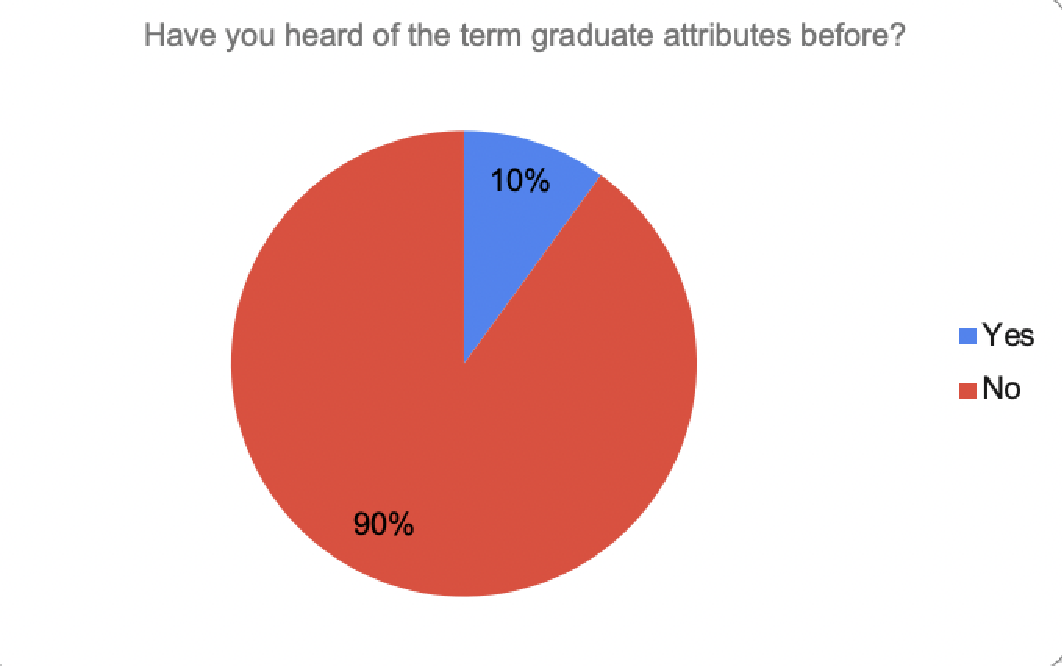
\includegraphics[scale=0.5]{images/GradAttr-1.pdf}
    \caption{Breakdown of the responses to the question "Have you heard of the term graduate attributes before?"}
    \label{fig: GradAttr-1}
    \end{centering}
\end{figure}

\begin{figure}[H]
    \begin{centering}
    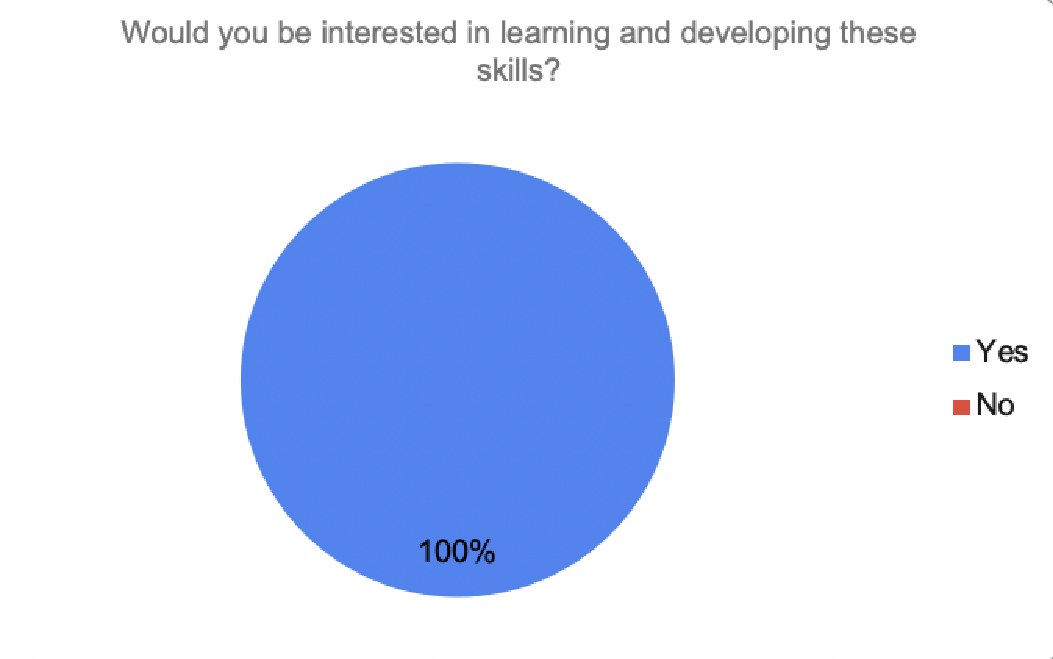
\includegraphics[scale=0.5]{images/GradAttr-2.pdf}
    \caption{Breakdown of the responses to the question "Would you be interested in learning and developing these skills?"}
    \label{fig: GradAttr-2}
    \end{centering}
\end{figure}

\begin{figure}[H]
    \begin{centering}
    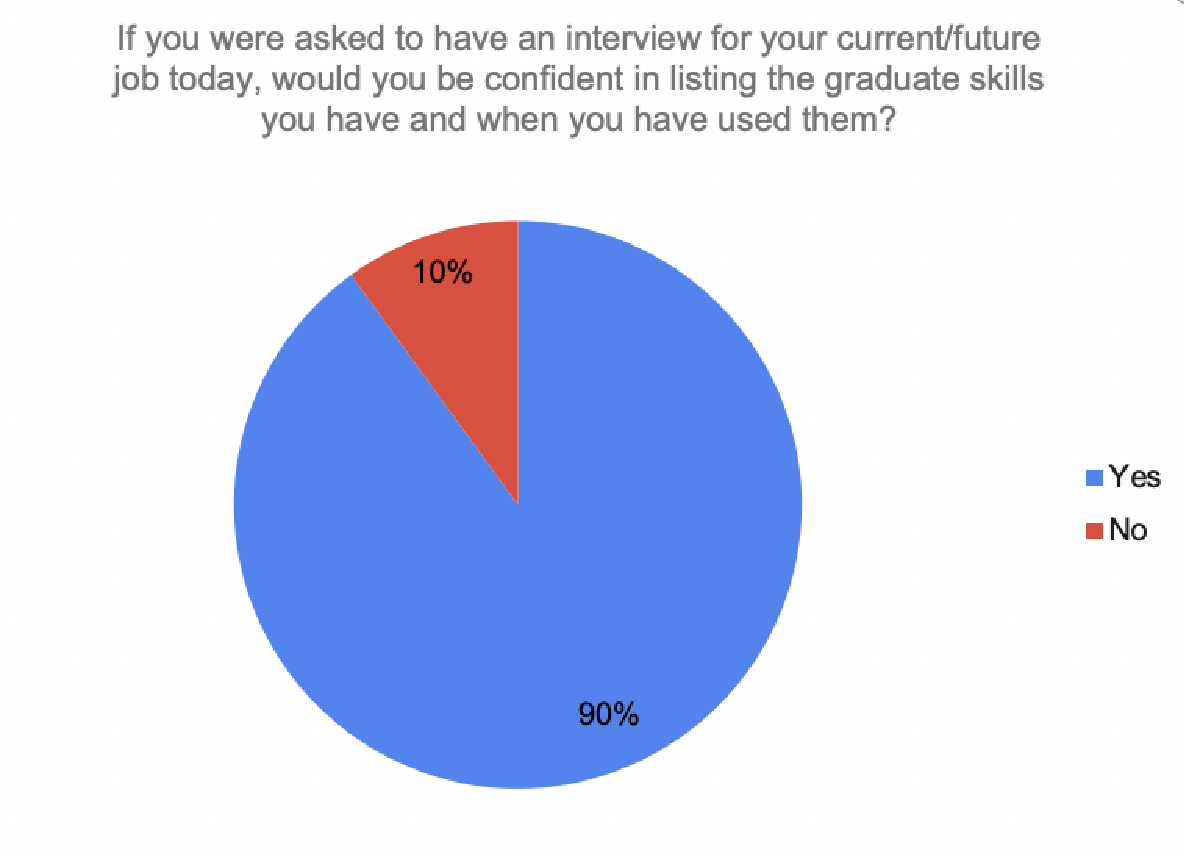
\includegraphics[scale=0.5]{images/GradAttr-3.pdf}
    \caption{Breakdown of the responses to the question "If you were asked to have an interview for your current/future job today, would you be confident in listing the graduate skills you have and when you have used them?"}
    \label{fig: GradAttr-3}
    \end{centering}
\end{figure}

\begin{figure}[H]
    \begin{centering}
    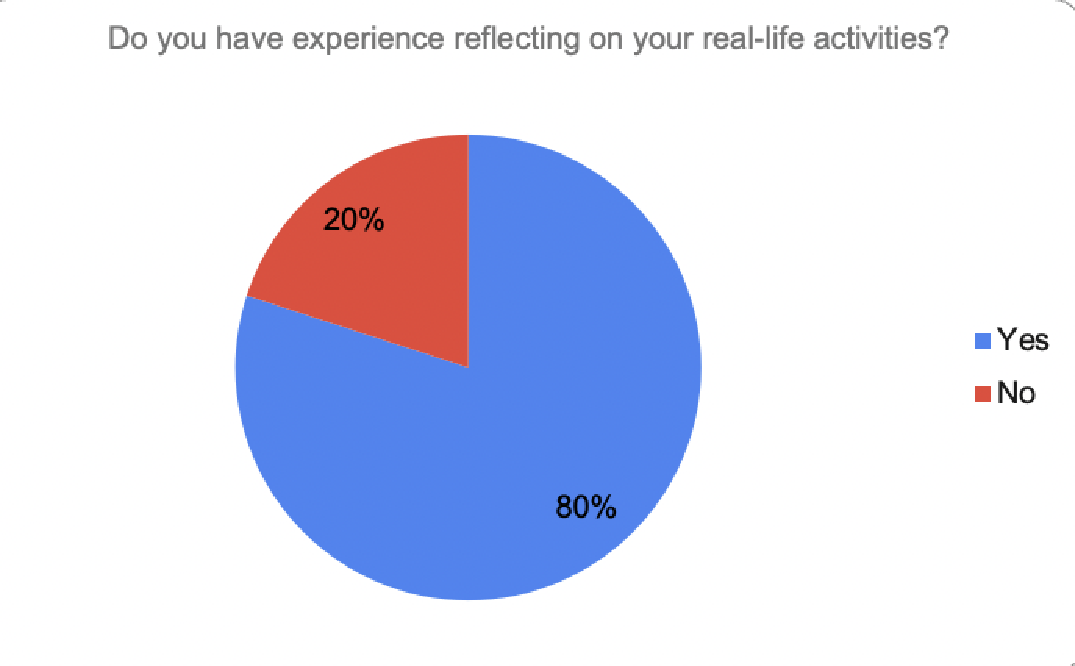
\includegraphics[scale=0.5]{images/GradAttr-4.pdf}
    \caption{Breakdown of the responses to the question "Do you have experience reflecting on your real-life activities?"}
    \label{fig: GradAttr-4}
    \end{centering}
\end{figure}

\begin{figure}[H]
    \begin{centering}
    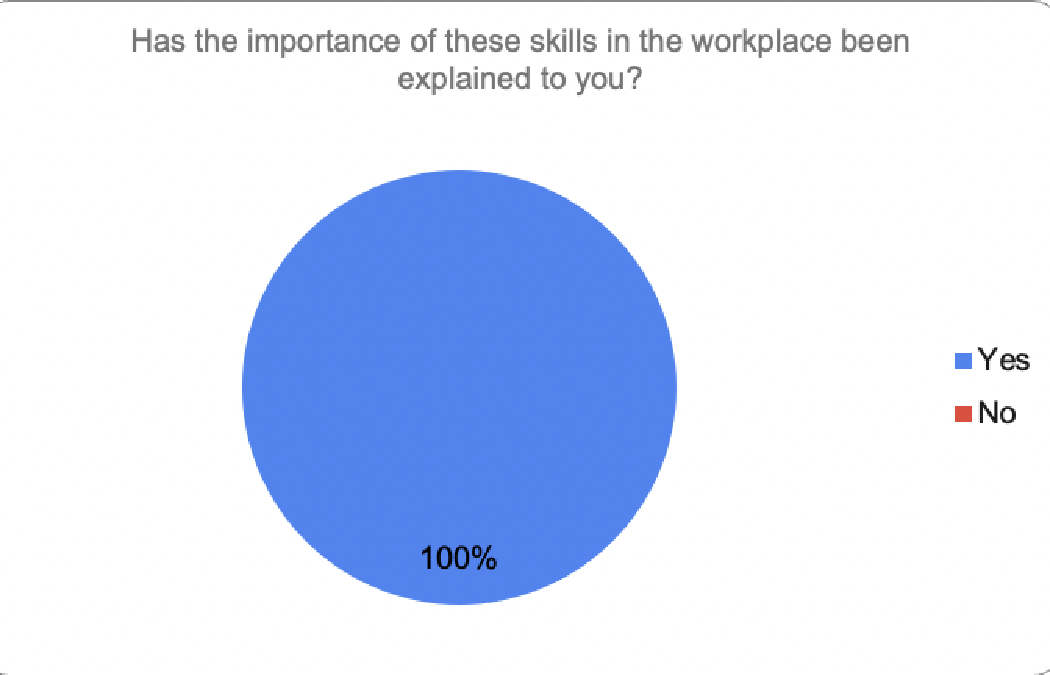
\includegraphics[scale=0.5]{images/GradAttr-5.pdf}
    \caption{Breakdown of the responses to the question "Has the importance of these skills in the workplace been explained to you?"}
    \label{fig: GradAttr-5}
    \end{centering}
\end{figure}

\begin{figure}[H]
    \begin{centering}
    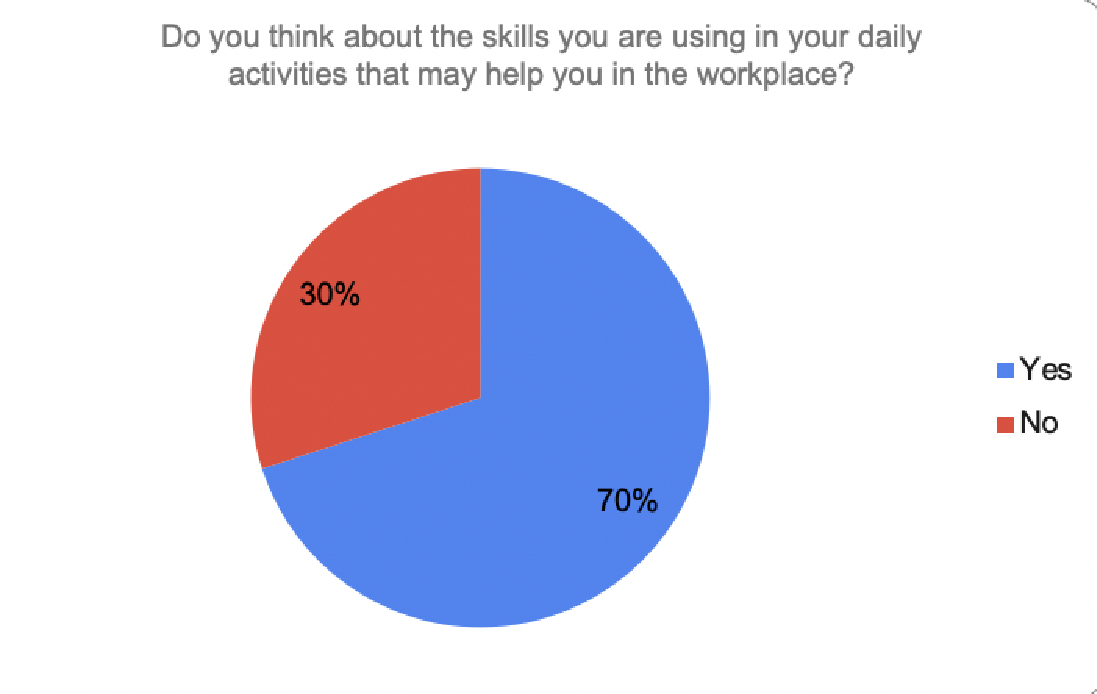
\includegraphics[scale=0.5]{images/GradAttr-6.pdf}
    \caption{Breakdown of the responses to the question "Do you think about the skills you are using in your daily activities that may help you in the workplace?"}
    \label{fig: GradAttr-6}
    \end{centering}
\end{figure}

\begin{figure}[H]
    \begin{centering}
    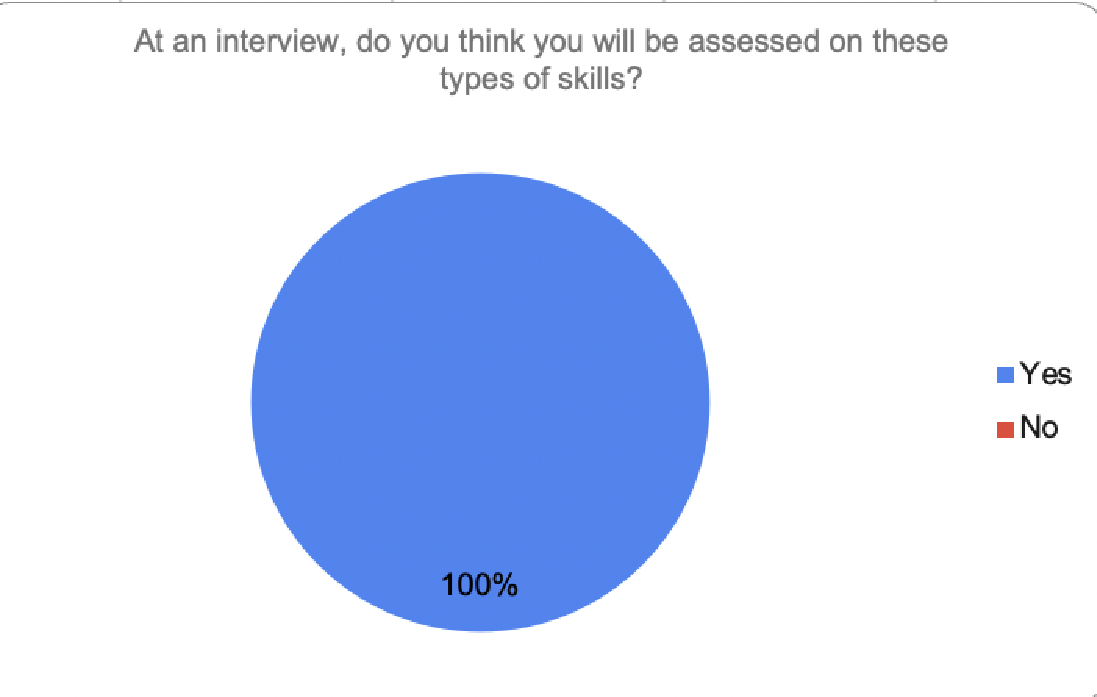
\includegraphics[scale=0.5]{images/GradAttr-7.pdf}
    \caption{Breakdown of the responses to the question "At an interview, do you think you will be assessed on these types of skills?"}
    \label{fig: GradAttr-7}
    \end{centering}
\end{figure}

\begin{figure}[H]
    \begin{centering}
    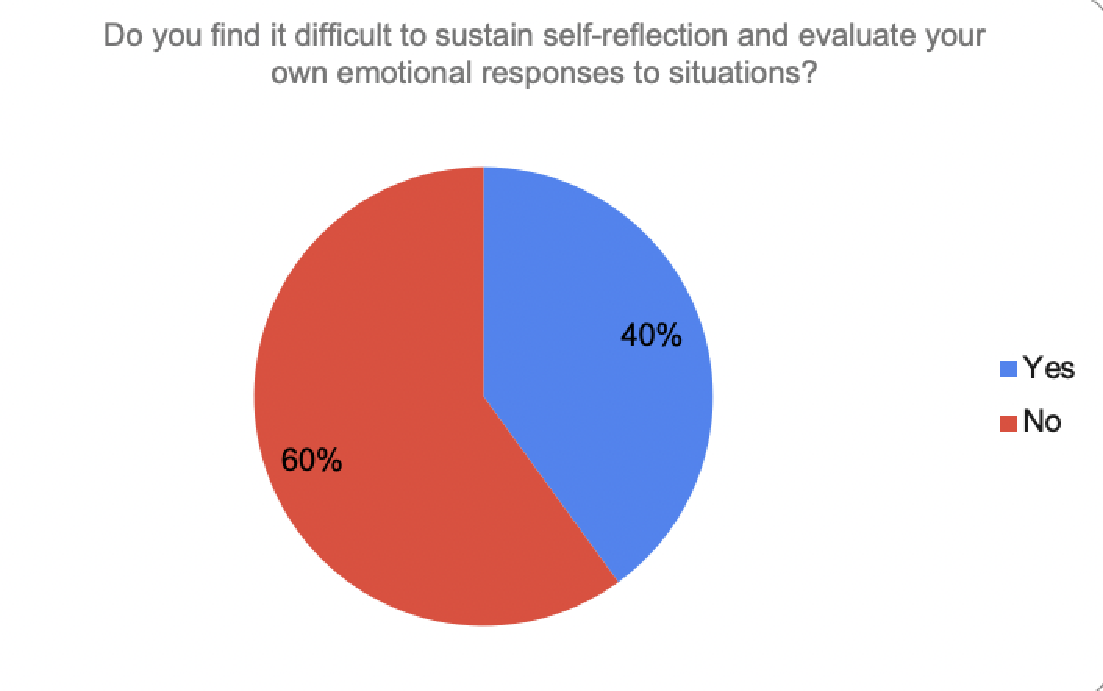
\includegraphics[scale=0.5]{images/GradAttr-8.pdf}
    \caption{Breakdown of the responses to the question "Do you find it difficult to sustain self-reflection and evaluate your own emotional responses to situations?"}
    \label{fig: GradAttr-8}
    \end{centering}
\end{figure}

\subsection{Comments by each participant after each question}

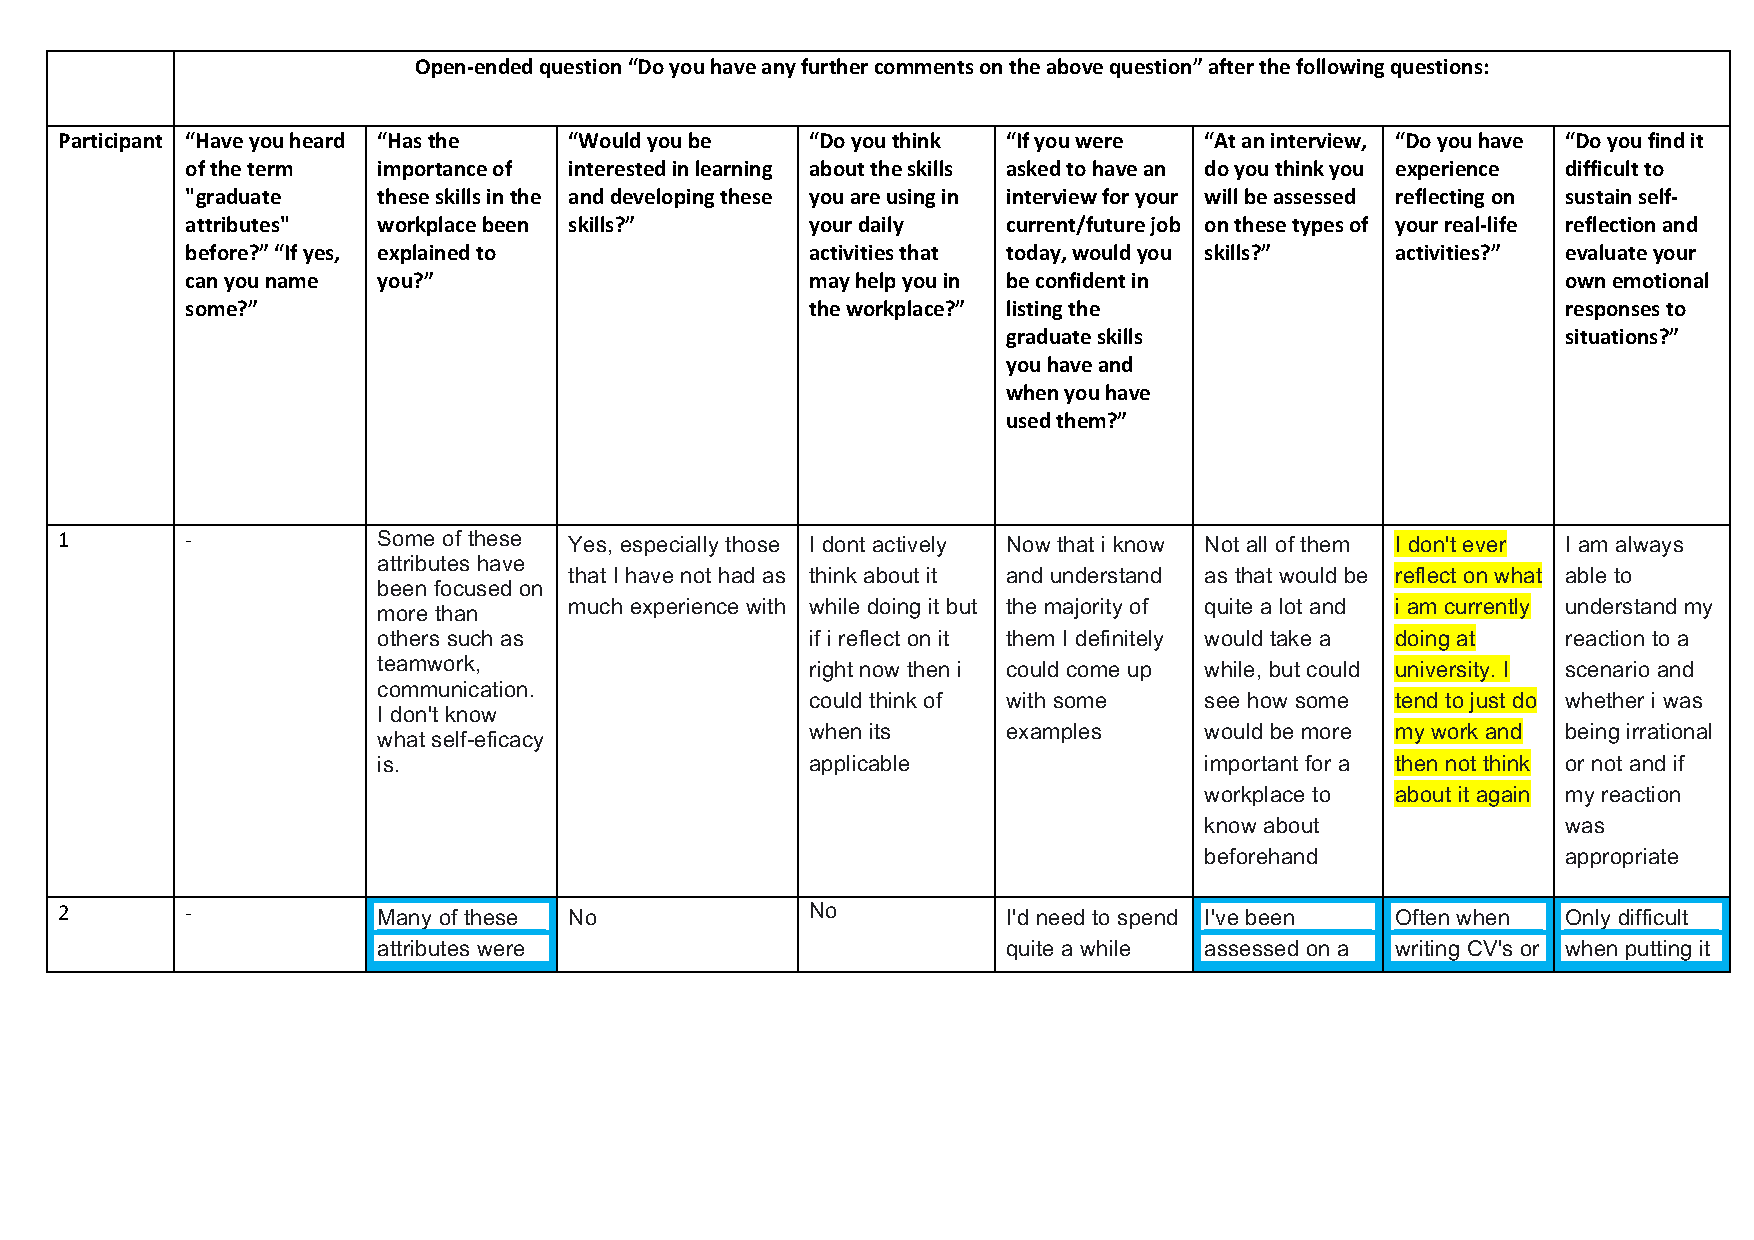
\includepdf[pages=-,pagecommand={},width=\textwidth, angle =90]{images/PDF_GeneralAttributeSurvey.pdf}

%==================================================================================================================================
%

\section{AB Tests} \label{Appendix-ABTests}

\subsection{Intro Script for both groups}
SCHOOL OF COMPUTING SCIENCE - UNIVERSITY OF GLASGOW

The aim of this experiment is to gain an understanding of what style of questions provokes the most reflection in students. 

We cannot get an understanding of this without participation from the students who would be answering these questions in an app being developed to aid reflection. 

You have been randomly allocated a group, the two groups will be answering two different styles of questions. 

You should answer the questions honestly, giving any extra comments where they feel appropriate.

The answers will be collected and analysed against the other group. 

Please ask questions if you need to, I will be available during and after the survey by email.

Please remember that this is to evaluate the effectiveness of the questions, and is in no way an evaluation on you, the participant.

You are able to withdraw from the survey at any time.

Below is a question asking for your consent to participate in this survey requiring you to select yes to continue, however if you do not consent, just close the survey at this point.

Please remember questions can be asked at any time.


Thank you.

\subsection{Questions for CBT group}

You will be asked to reflect based on an experience where you feel you have developed on one of these skills:

- Communication
- Critical thinking
- Adaptability
- Teamwork
- Self-efficacy
- Application of knowledge
- Ethics
- Professionalism 

Throughout the survey, an example of an experience where someone settled a dispute between members of their team will be used to assist in your own reflection.

\begin{enumerate}
    \item What graduate skill did you develop?
    \item Describe a situation in which you developed this skill. [The situation is the concrete experience, this only covers the facts of what happened with no interpretation. An example could include settling a dispute between peers for Teamwork]
    \item What were your thoughts during this experience? [Thoughts help to interpret a situation, there are different ways to interpret a single situation. These thoughts can be positive or negative. For example, that you were thinking that a dispute between your peers could cause delays further down the line, that you thought it could damage the overall harmony of the team, etc]
    \item How did you feel during this situation? [These emotions will be based on your thoughts about the experience and can be both negative and positive. This scale does not describe the scenario, but instead your emotional response to the experience.]
    \item Why do you think you felt this way? [Reasons behind your emotions can stem from many things, it could be as a result of previous experiences, foreseeable impacts, etc. Continuing the team dispute example, a reason someone would feel negatively about the team dispute could be that it has happened in a previous team and resulted in a bad team environment, an example of why they could feel positively about it could be that it gave them the opportunity to take on a proactive role in settling the dispute and creating a good environment or their team.]
    \item How did you behave in this experience? [This requires you to examine the cause and effect.  How does the resulting behaviour directly relate to your thoughts and feelings? For example, someone taking the two arguing team members aside and discussing with them how to sort the dispute and compromise. This could be because they did not want to ruin the team environment that had been positive up until the dispute, and wanted to create the best product they could as a team.]
    \item How would you want to behave in the future? Would you act the same or differently, and why? [Here we are examining alternate thought. You have to examine all of your previous answers and decide if this is how you would handle another similar situation and whether the behaviour you had resulted in the best possible outcome. This will help you to make new connections and create different, more positive experiences in the future. For example, someone might behave in the same way in settling the dispute, however they may act sooner next time to ensure there is no impact on team cohesion.]
    \item 
\end{enumerate}

\subsection{Questions for control group}

\begin{enumerate}
    \item Describe an achievement you are proud of
    \item Describe a time you showed professionalism
    \item Describe a time where you had to use your ethical skills
    \item What skills are your strongest?
    \item What areas can you improve in?
    \item Describe a time when you made a mistake
    \item How would you handle a team conflict?
\end{enumerate}

\subsection{Debrief script for CBT group}

The main aim of this experiment was to gain an understanding of what style of questions provokes the most reflection in students. 

You were in group A, the experimental group. I was particularly interested in seeing if answering this style of questions, based closely off of a form of therapy called CBT which encourages reflection, would provoke deeper reflection from participants. 

The other group were the control group. These participants were given questions based on simple job interview questions.

Please take a note of my email address, and please let me know if you have any further questions about this experiment.

Gemma McDonald
2306631m@student.gla.ac.uk

Thank you for your help.


\subsection{Debrief script for control group}

The main aim of this experiment was to gain an understanding of what style of questions provokes the most reflection in students. 

You were in group B, the control group. I was particularly interested in seeing if answering this style of questions,  based closely off of simple job interview questions, would give less reflection from participants then group A, the experimental group.

The other group, the experimental group, were given questions based closely off of a form of therapy called CBT which encourages reflection.

Please take a note of my email address, and please let me know if you have any further questions about this experiment.

Gemma McDonald
2306631m@student.gla.ac.uk

Thank you for your help.


\subsection{Graphs}

\begin{figure}[H]
    \begin{centering}
    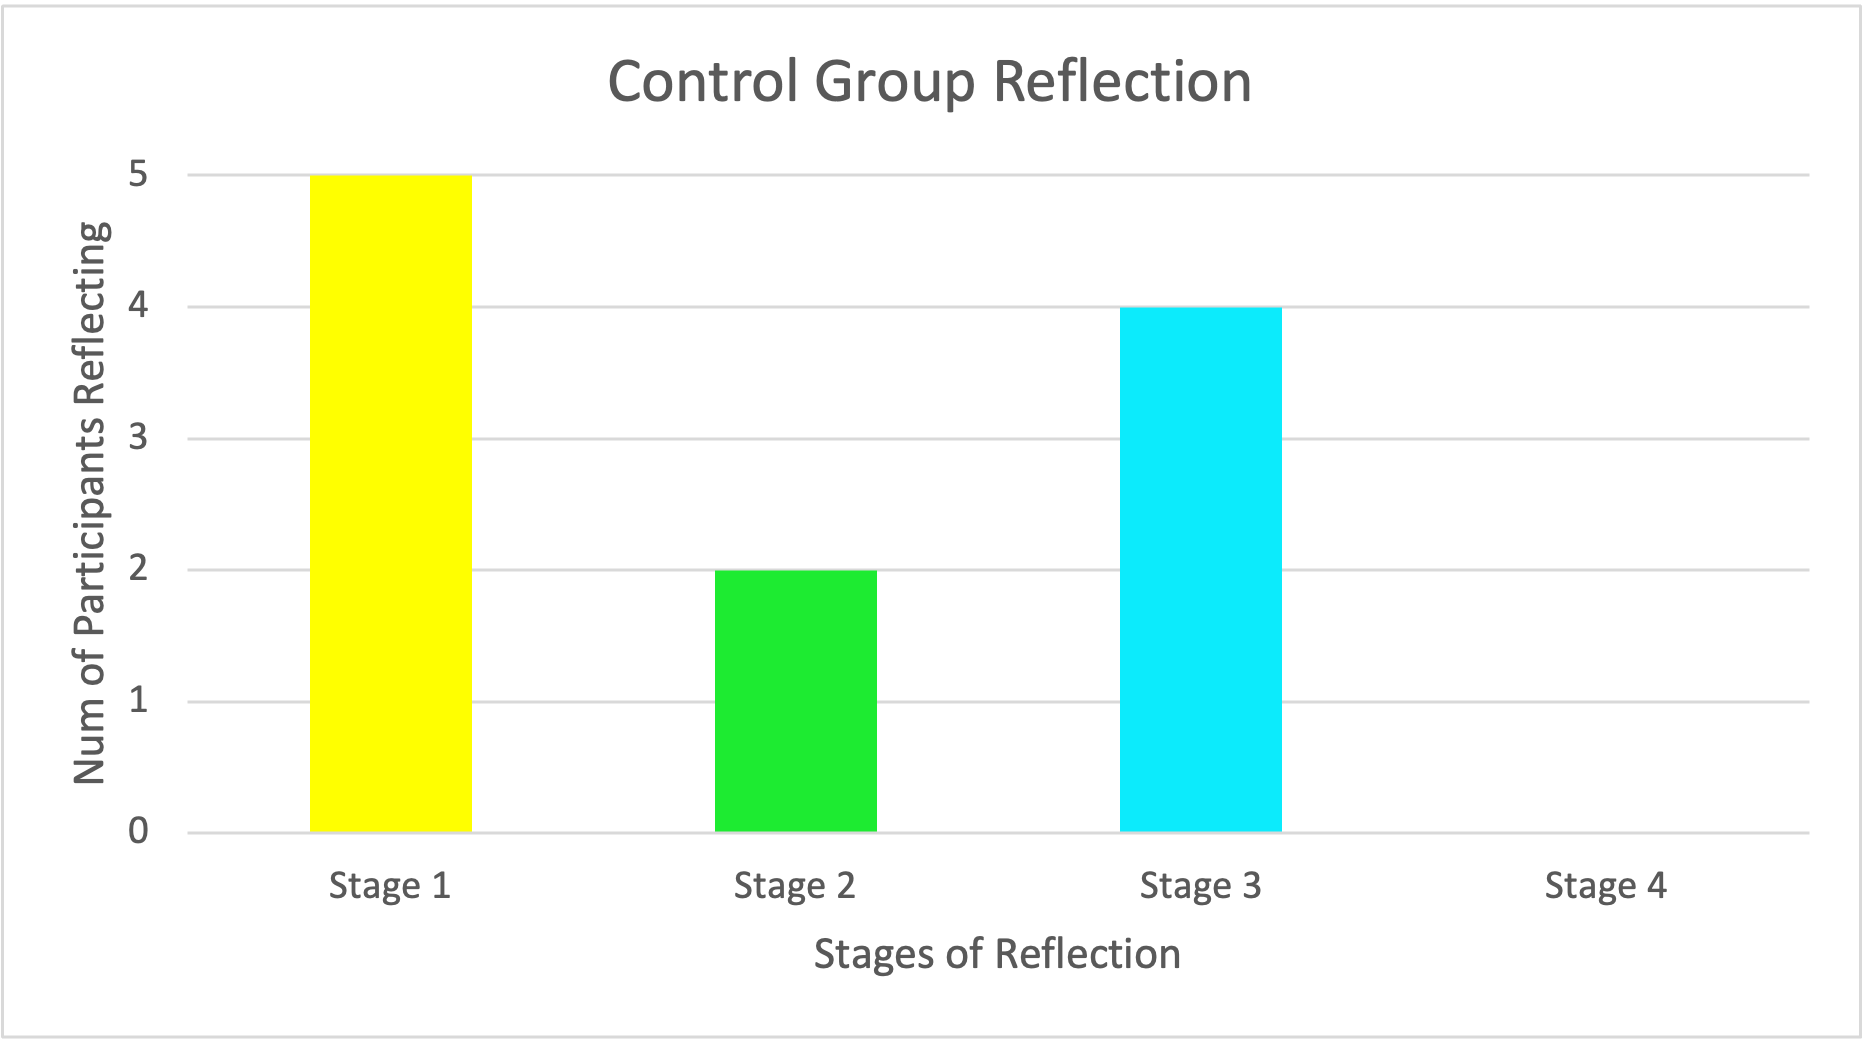
\includegraphics[scale=0.5]{images/ABControlGraph.png}
    \caption{Graph showing the levels of reflection the participants reach for the control group using the job interview questions.}
    \label{fig: Appen-ControlGraph}
    \end{centering}
\end{figure}

\begin{figure}[H]
    \begin{centering}
    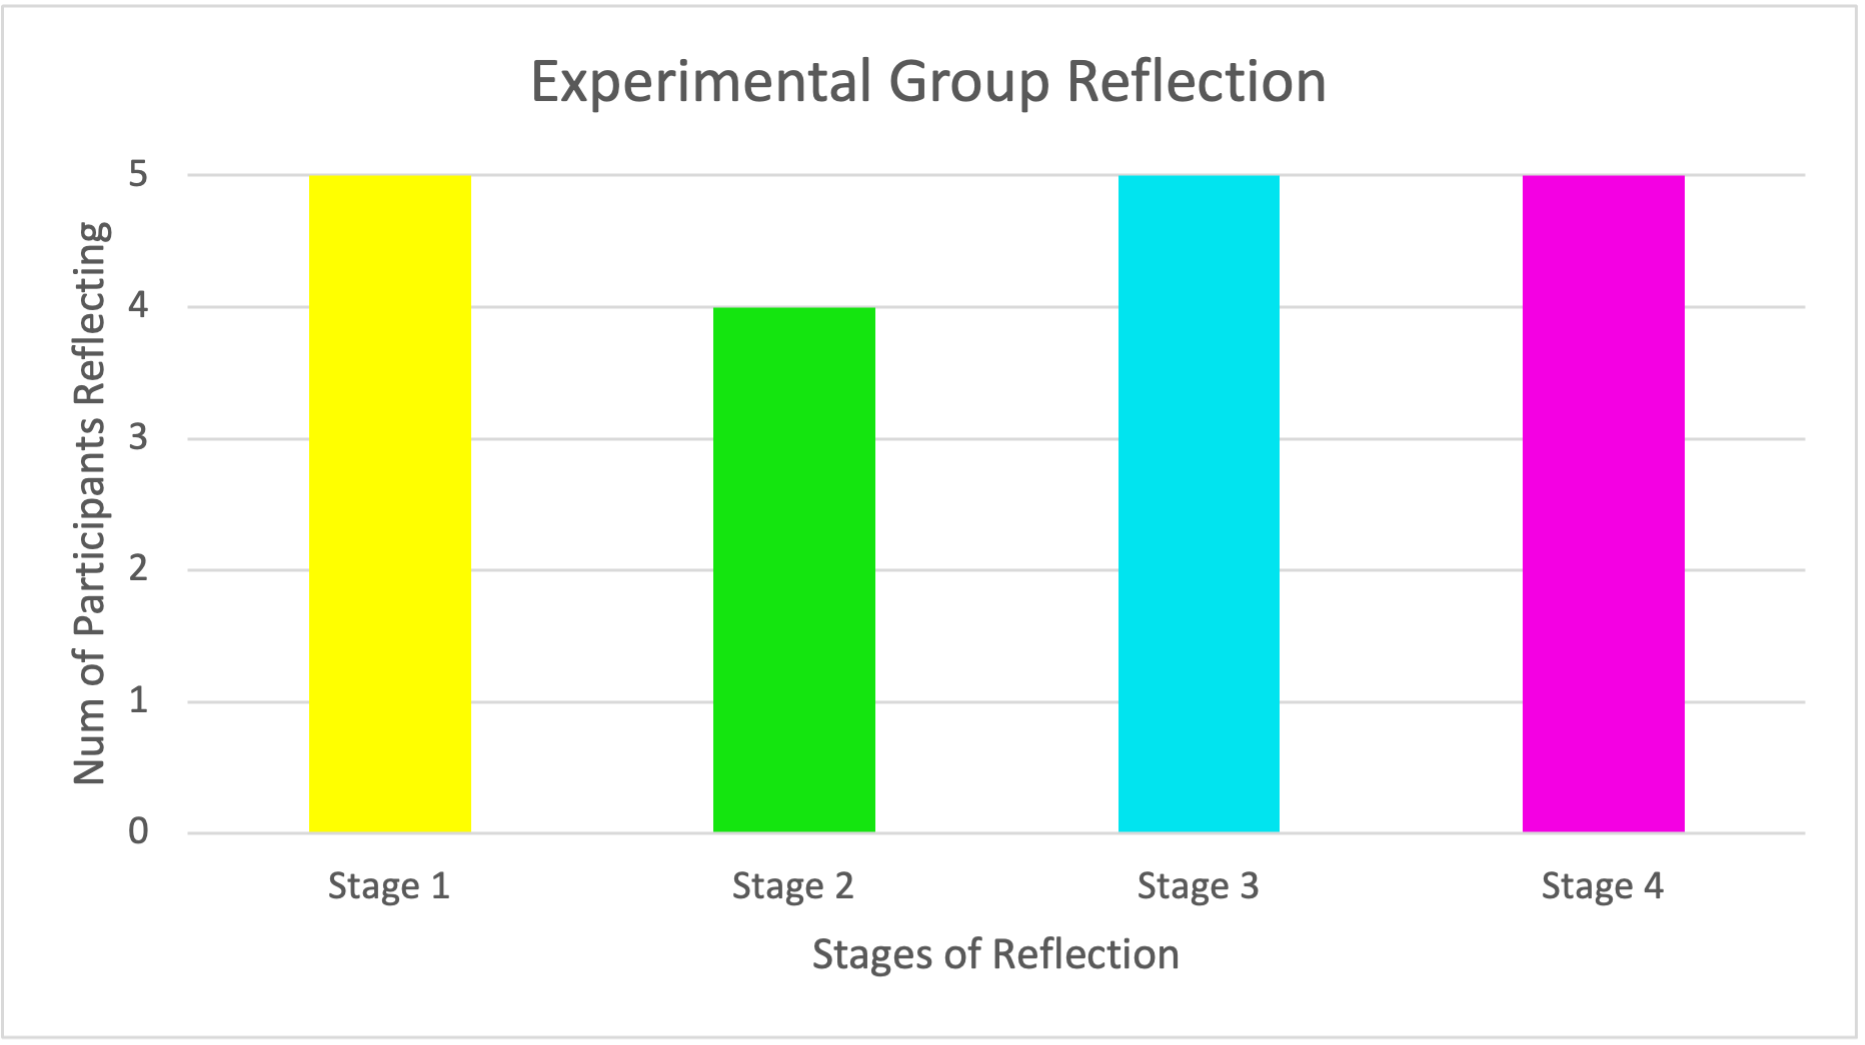
\includegraphics[scale=0.5]{images/ABExperimentGraph.png}
    \caption{Graph showing the levels of reflection the participants reach for the experiment group using the CBT questions.}
    \label{fig: Appen-ExperimentGraph}
    \end{centering}
\end{figure}

\subsection{Breakdown of the responses showing the colour coding for each level of reflection} \label{Appendix-AB-responses}

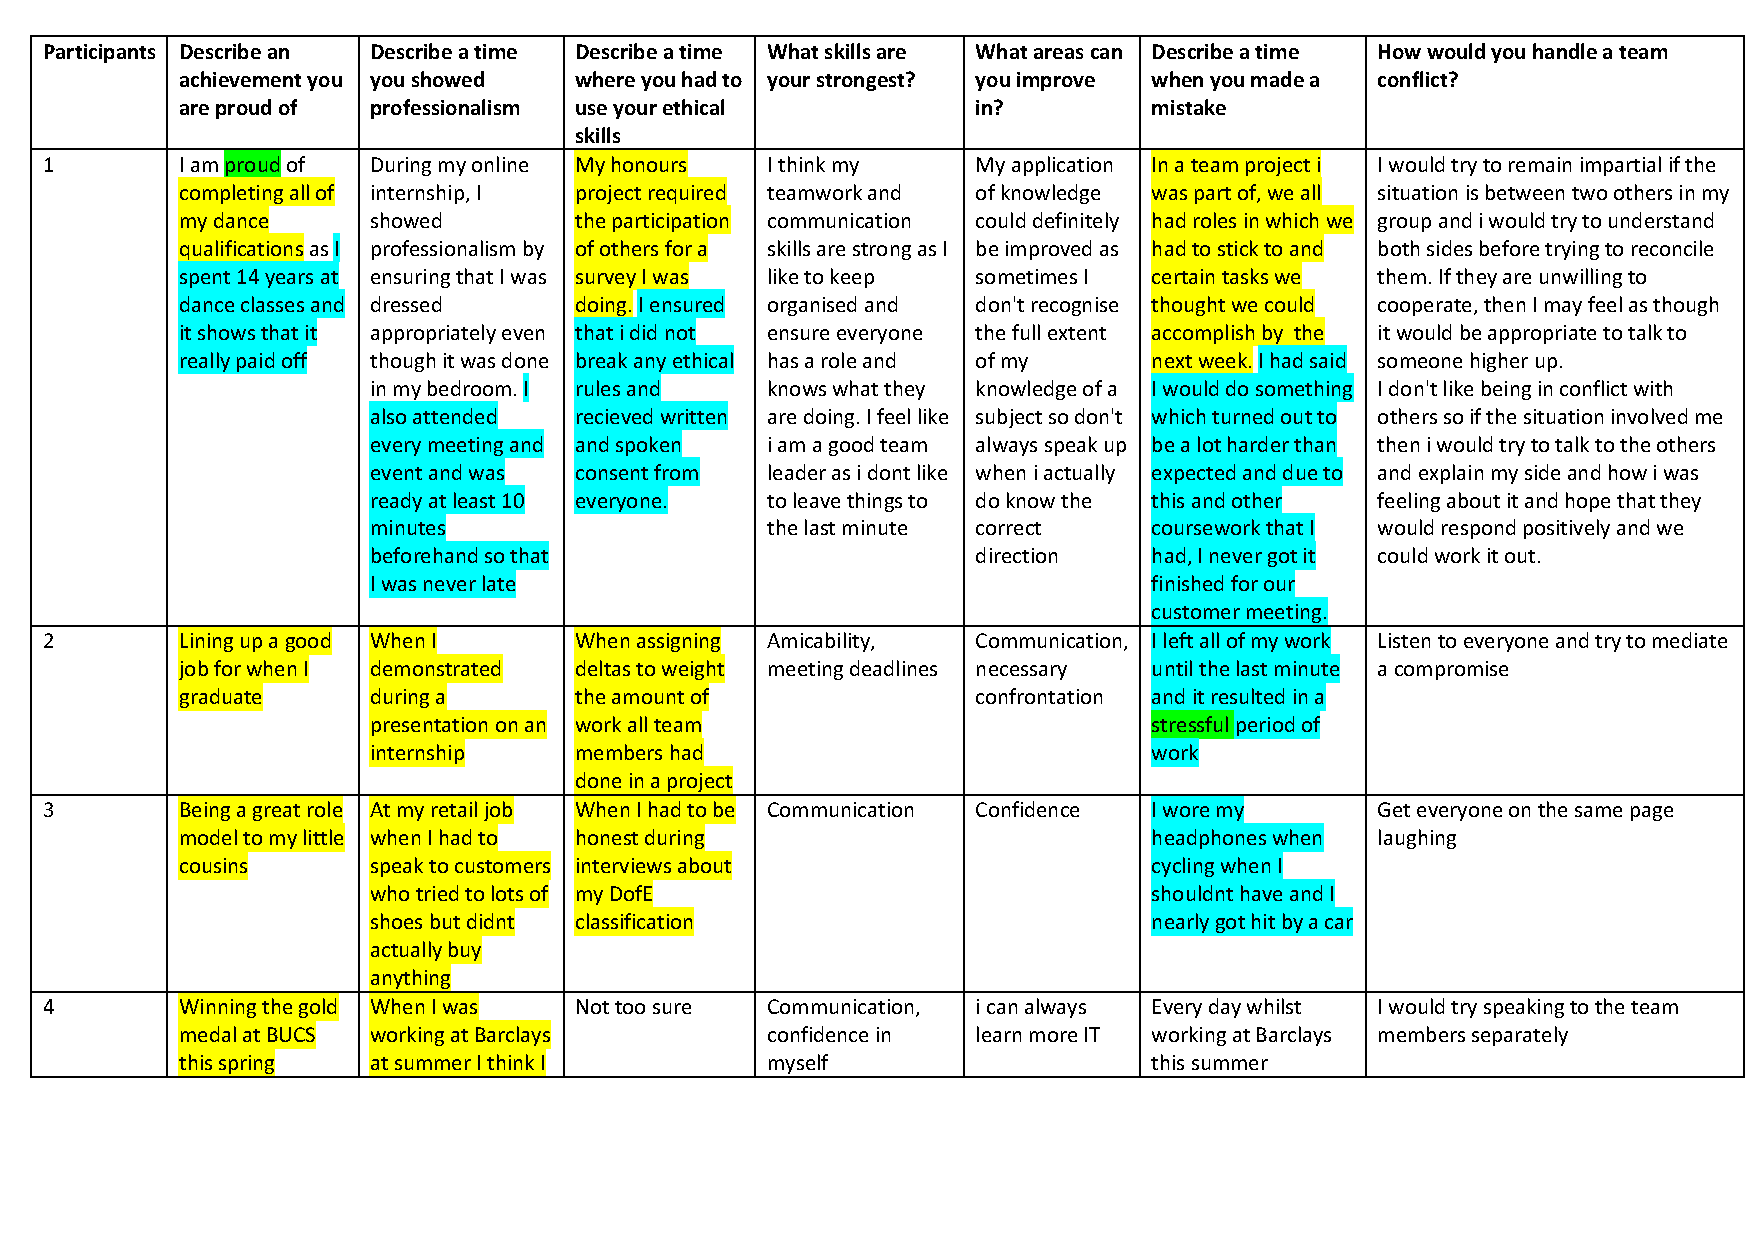
\includepdf[pages=-,pagecommand={},width=\textwidth, angle =90]{images/ProcessedControlGroupCoding.pdf}

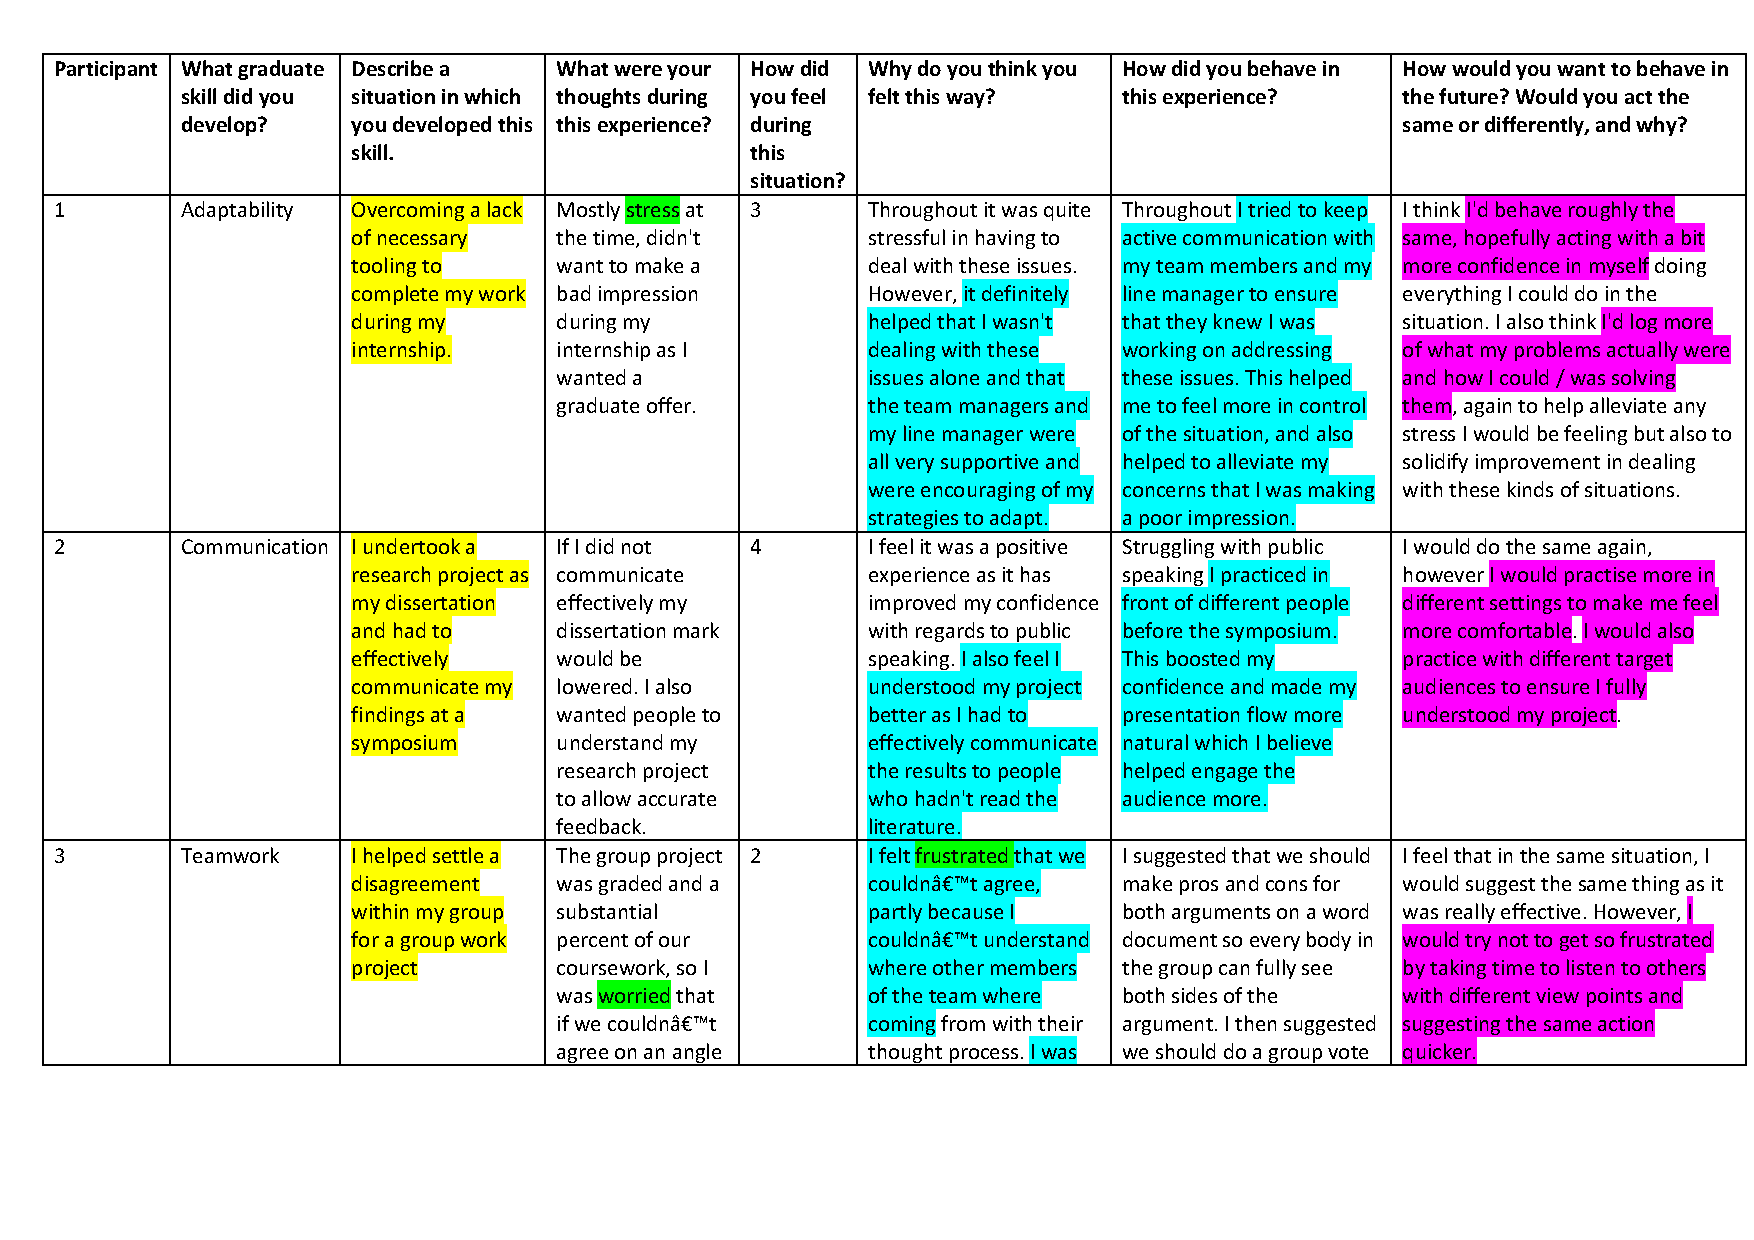
\includepdf[pages=-,pagecommand={},width=\textwidth, angle =90]{images/ProcessedExperimentalGroupCoding.pdf}

%==================================================================================================================================
%
\section{User personas} \label{Appendix-userPersonas}

\textbf{Types of users}
\begin{itemize}
    \item Student
    \item Recent graduate
    \item Experienced member of a workplace
    \item Intern/Apprentices
\end{itemize}

\textbf{Personas}
\begin{itemize}
    \item \textbf{Steven} Steven is an Intern doing his first ever technology internship. Through different speaker sessions during the internship he has heard all the different skills he needs to work well within the company. He's concerned he hasn't had the opportunity to develop these skills as he has never heard about graduate skills.
    \item \textbf{Maisie} Maisie is a student currently in her third year of university studying computing science. She has been working on her third year team project with some fellow students and is looking for a way to keep track of the skills she's using throughout the project so she can refer to them in her CV later. She knows these skills will be important for her in the workplace and is keen to start tracking her development early.
    \item \textbf{Michael} Michael has been working in the same position in his workplace for the last 5 years and is looking to put himself up for promotion soon, however its been a long time since he had an interview and is concerned he will not be able to promote himself well in the interview. He needs a way to gather together the many skills he has gained through years of working in the company and be able to review them before his interview. He wants to make sure he continues to work on his personal development.
    \item \textbf{Abigail} Abigail has just graduated university and is just about to start her new job. She wants to be able to make sure she stays on top of all the skills she learns on the job as she has aspirations of advancing quickly through the company. She needs to be reminded to journal about her experiences, and continue to grow and develop her skills within the company.
\end{itemize}

%==================================================================================================================================
%

\section{User Stories} \label{Appendix-userStories}

As an intern, I want to be able to learn what graduate skills are, so that I can develop on them.

As an intern, I want to be able to keep track of the real-world experiences from my internship, so that I can recognise the skills I am developing.

As student, I want to be able to know how to reflect on the experiences I am having during the team project, so that I can keep up with my CV.

As a student, I want to be able to become more aware of my skills and when I am using them, so that I can perform well in a job interview.

As a student, I want to be able to become more aware of my skills and when I am using them, so that I can work efficiently in my future workplace.

As a student, I want to be able to take convenient and quick recordings of my experiences, so that I can capture them on the go and go back to them later.

As a student, I want to be able to see what skill I have developed and what skills require more development, so that I can focus my attention on seeking opportunities to develop more skills and provide value to my future workplace.

As a student, I want to have an explanation of how to reflect on my skills in a beneficial way, so that I know what I am doing and can reflect effectively.

As an experienced member of the workplace, I want to be able to be able to save journal entries and refresh myself on what my key experiences and skills are, so that I can get my promotion.

As an experienced member of the workplace, I want to continue to work on my skills, so that I can continue to improve my personal growth and provide value to the workplace.

As a graduate, I want to be able to have a reminder to reflect on all my skills, so that I can progress my career.

As a graduate, I want to be fully prepared to join the workplace and have developed my key graduate skills, so that I can feel confident and provide value to my teams.

%==================================================================================================================================
%

\section{CBT questions and Prompts from App} \label{Appendix-AppCBTQuestions-Prompts}

\begin{center}
    \begin{tabular}{ | m{8em} | m{10cm}| } 
    \hline
    \textbf{Question} & \textbf{Prompt} \\ [0.5ex] 
    \hline\hline
    Note Title: & Give your note a title, this is how the note will be stored for reviewing later \\ 
    \hline
    What graduate skill did you develop? & You will be asked to reflect based on an experience where you feel you have developed on one of these skills. Throughout the survey, an example of an experience where someone settled a dispute in their team will be used to assist in your own reflection. \\
    \hline
    Describe the situation in which you developed this skill & The situation is the concrete experience, this only covers the facts of what happened with no interpretation. An example could include settling a dispute between peers for Teamwork \\
    \hline
    What were your thoughts during this experience? & Thoughts help to interpret a situation, there are different ways to interpret a single situation. These thoughts can be positive or negative. For example, thinking that a dispute between your peers could cause delays further down the line, thinking it could damage the overall harmony of the team, etc \\
    \hline
    How did you feel during this situation? & These emotions will be based on your thoughts about the experience and can be both negative and positive. This scale does not describe the scenario, but instead your emotional response to the experience. \\
    \hline
    Why do you think you felt this way? & The reasons behind your emotions can stem from many things, it could be the result of previous experiences, foreseeable impacts, etc. For example, in a team dispute, a person could feel negative because in a previous team it resulted in a bad working environment. An example of why they could feel positive could be that it gave them the opportunity to take a proactive role in settling the dispute, creating a good environment for their team. \\
    \hline
    How did you behave in this experience? & This requires you to examine the cause and effect.  How does the resulting behaviour directly relate to your thoughts and feelings? For example, someone taking two arguing team members aside and discussing how to compromise. This could be because they did not want to ruin the team environment that had been positive up until the dispute, and wanted to create the best product they could as a team. \\
    \hline
    How would you want to behave in the future? Would you act the same or differently, and why? & Here we are examining alternate thought. You have to examine all of your previous answers and decide if this is how you would handle a similar situation, and whether your behaviour resulted in the best possible outcome. This will help you to make new connections and create different, more positive experiences in the future. For example, someone might behave in the same way in settling the dispute, however they may act sooner next time to ensure there is no impact on team cohesion. \\ [1ex] 
    \hline
   \end{tabular}
   \end{center}



%==================================================================================================================================
%

\section{Paper Prototypes} \label{Appendix-PaperPrototypes}

\begin{figure}[H]
    \centering
    \begin{subfigure}[b]{1\textwidth}
        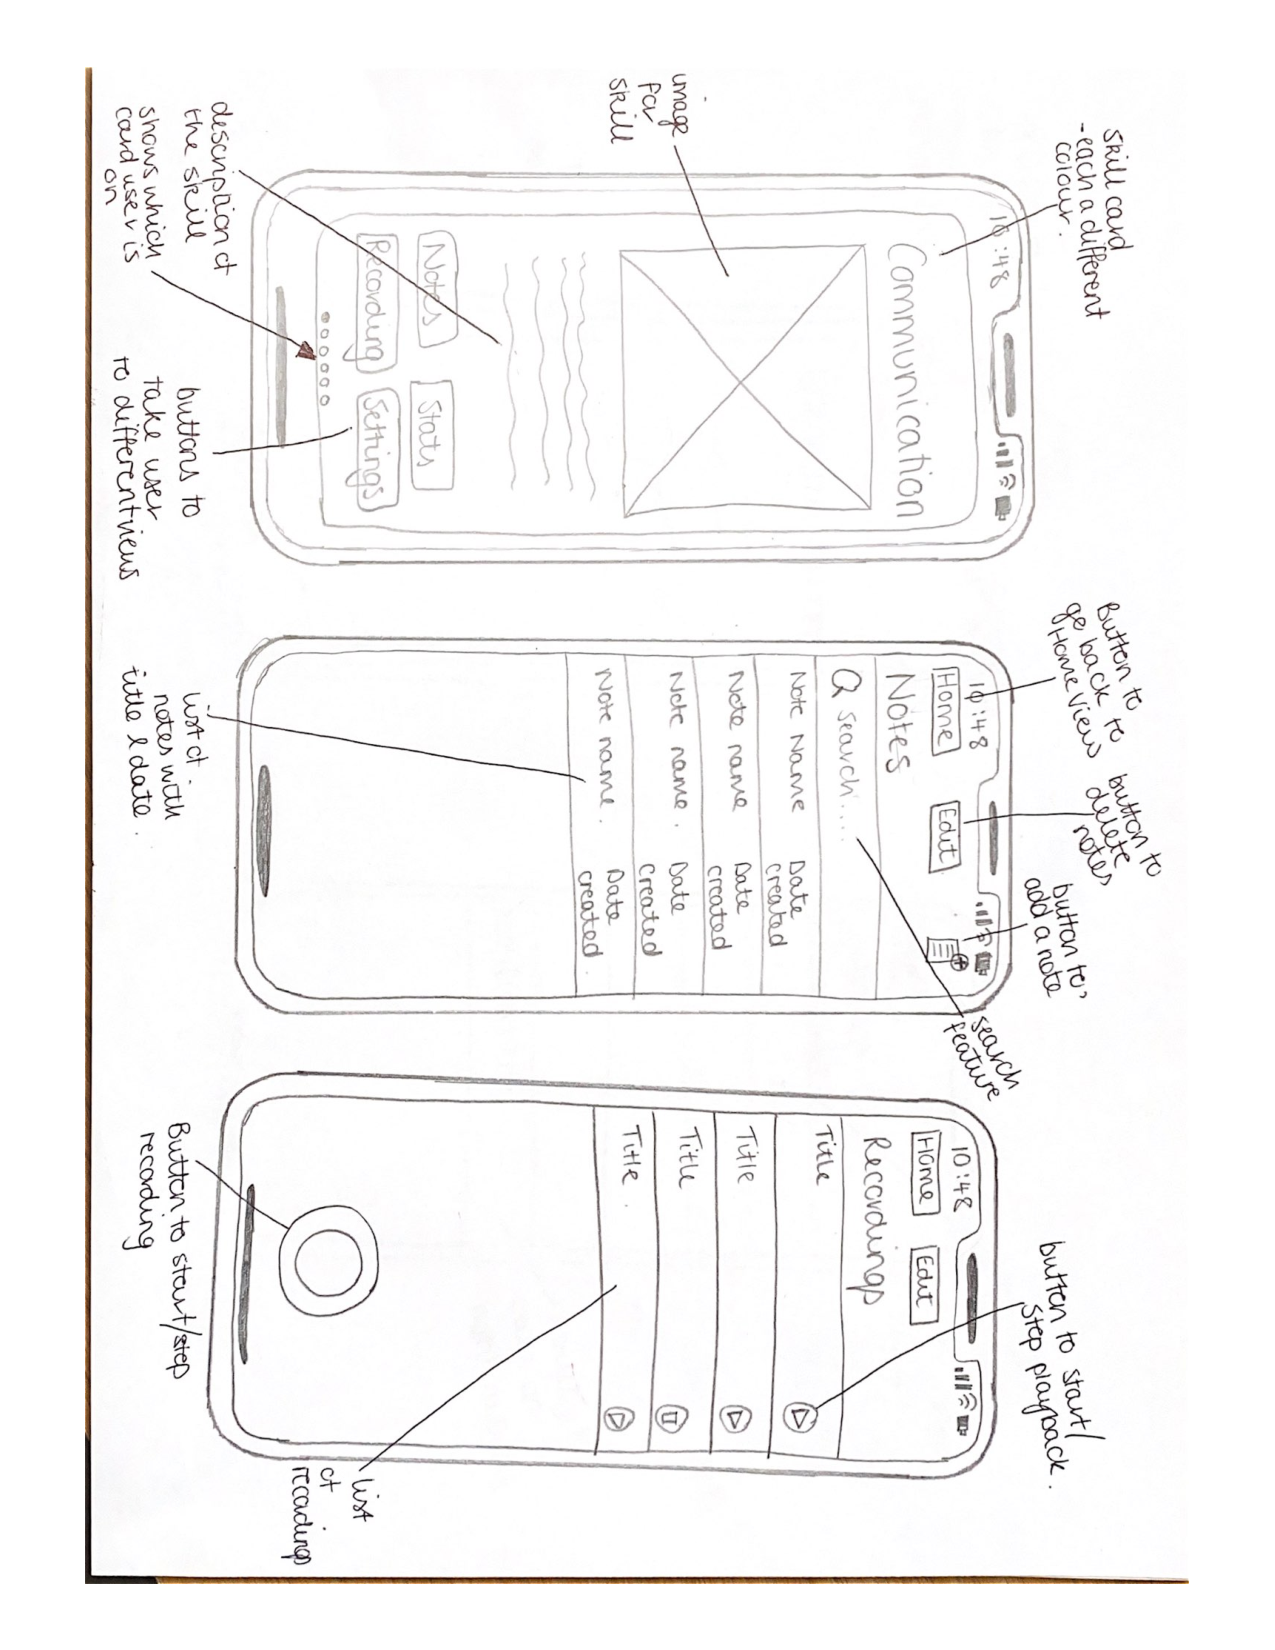
\includegraphics[scale=0.3, angle = 90]{images/PaperWireframes1.pdf}
        \caption{Initial paper prototype designs for the Home, Note and Recordings views.}
        \label{fig:PaperPrototype1}
    \end{subfigure}
    \begin{subfigure}[b]{1\textwidth}
        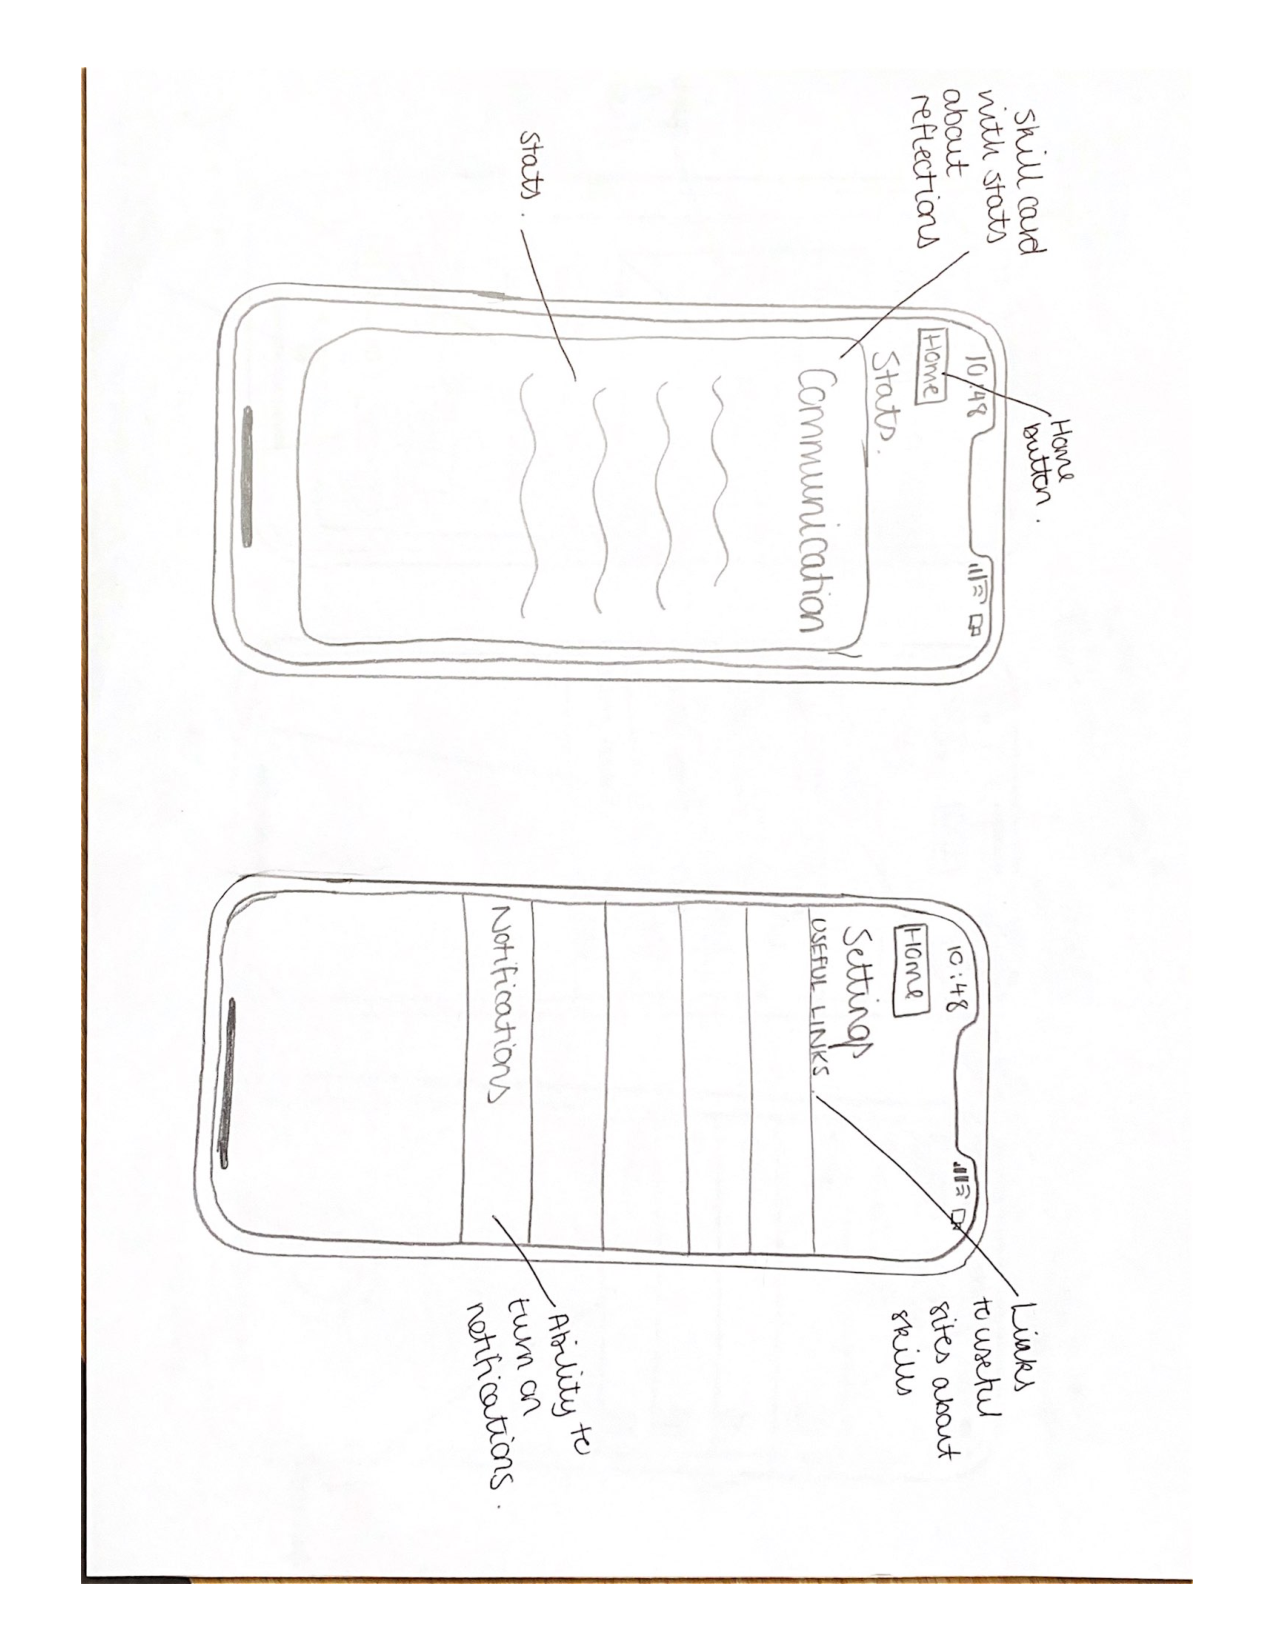
\includegraphics[scale=0.3, angle = 90]{images/PaperWireframes2.pdf}
        \caption{Initial paper prototypes for the Statistics and Settings view.}
        \label{fig:PaperPrototype2}
    \end{subfigure}     
    \caption{Scanned files showing the paper prototypes that were made in the early stages of design, iterative changes were made to the design for the final product.}
    \label{fig:PaperPrototypes}
\end{figure}

%==================================================================================================================================
%

\section{High Fidelity Wireframes}\label{Appendix-highFidelityWireframes}

\begin{figure}[H]
    \centering
    \begin{subfigure}[b]{0.3\textwidth}
        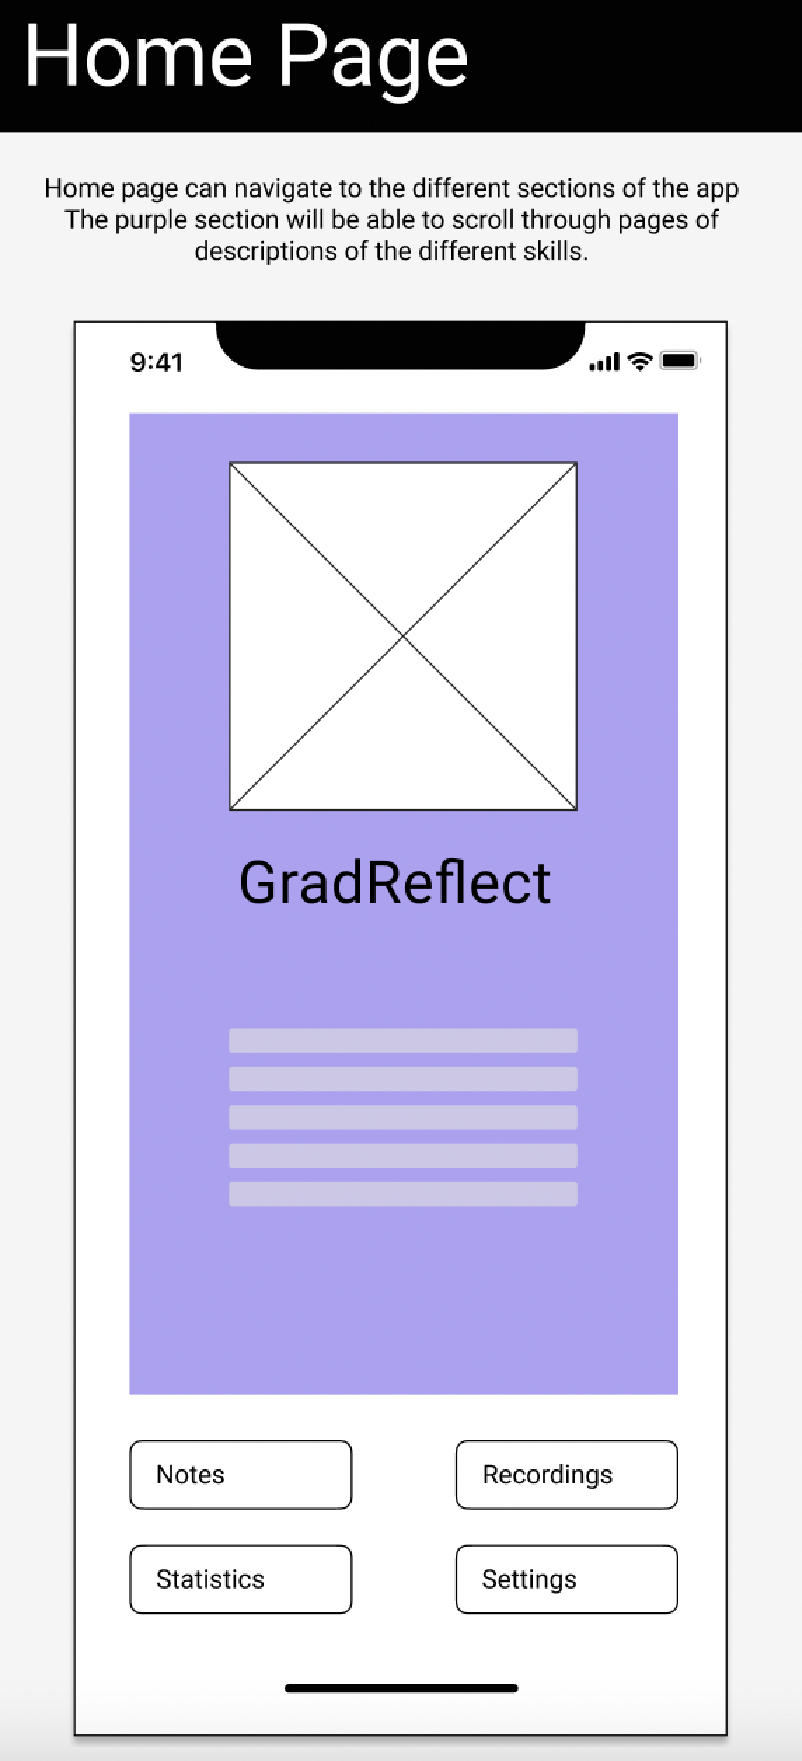
\includegraphics[scale=0.3]{images/HomeWireframe.pdf}
        \caption{High fidelity wireframe prototype design for the Home view.}
        \label{fig:HomeWireframe}
    \end{subfigure}
    \begin{subfigure}[b]{0.3\textwidth}
        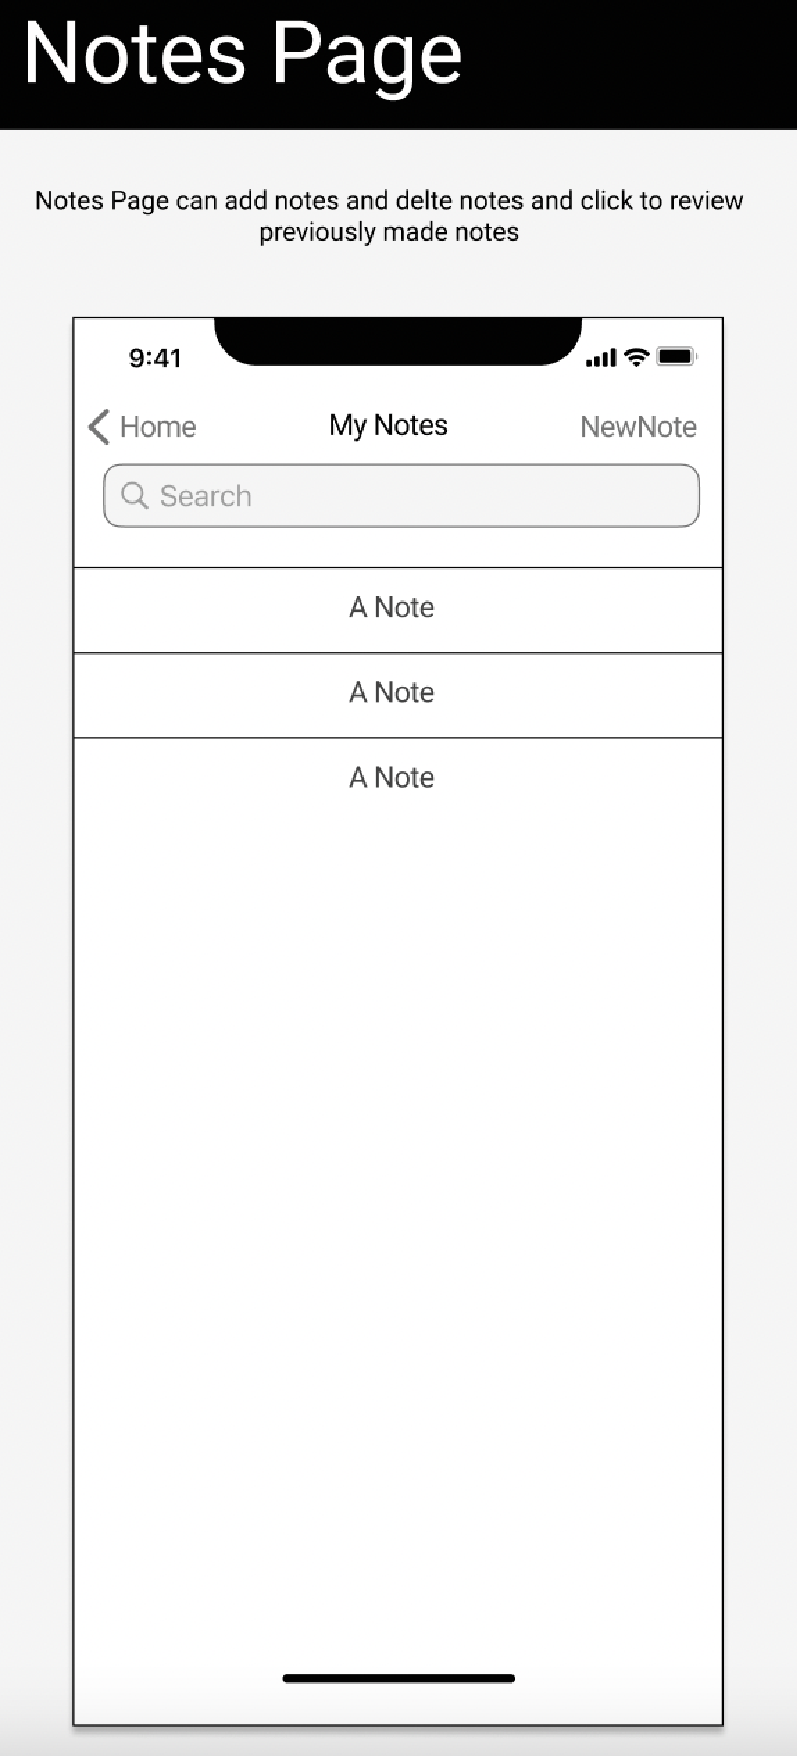
\includegraphics[scale=0.3]{images/NotesWireframe.pdf}
        \caption{High fidelity wireframe prototype design for the Notes view.}
        \label{fig:NotesWireframe}
    \end{subfigure}   
    \begin{subfigure}[b]{0.3\textwidth}
        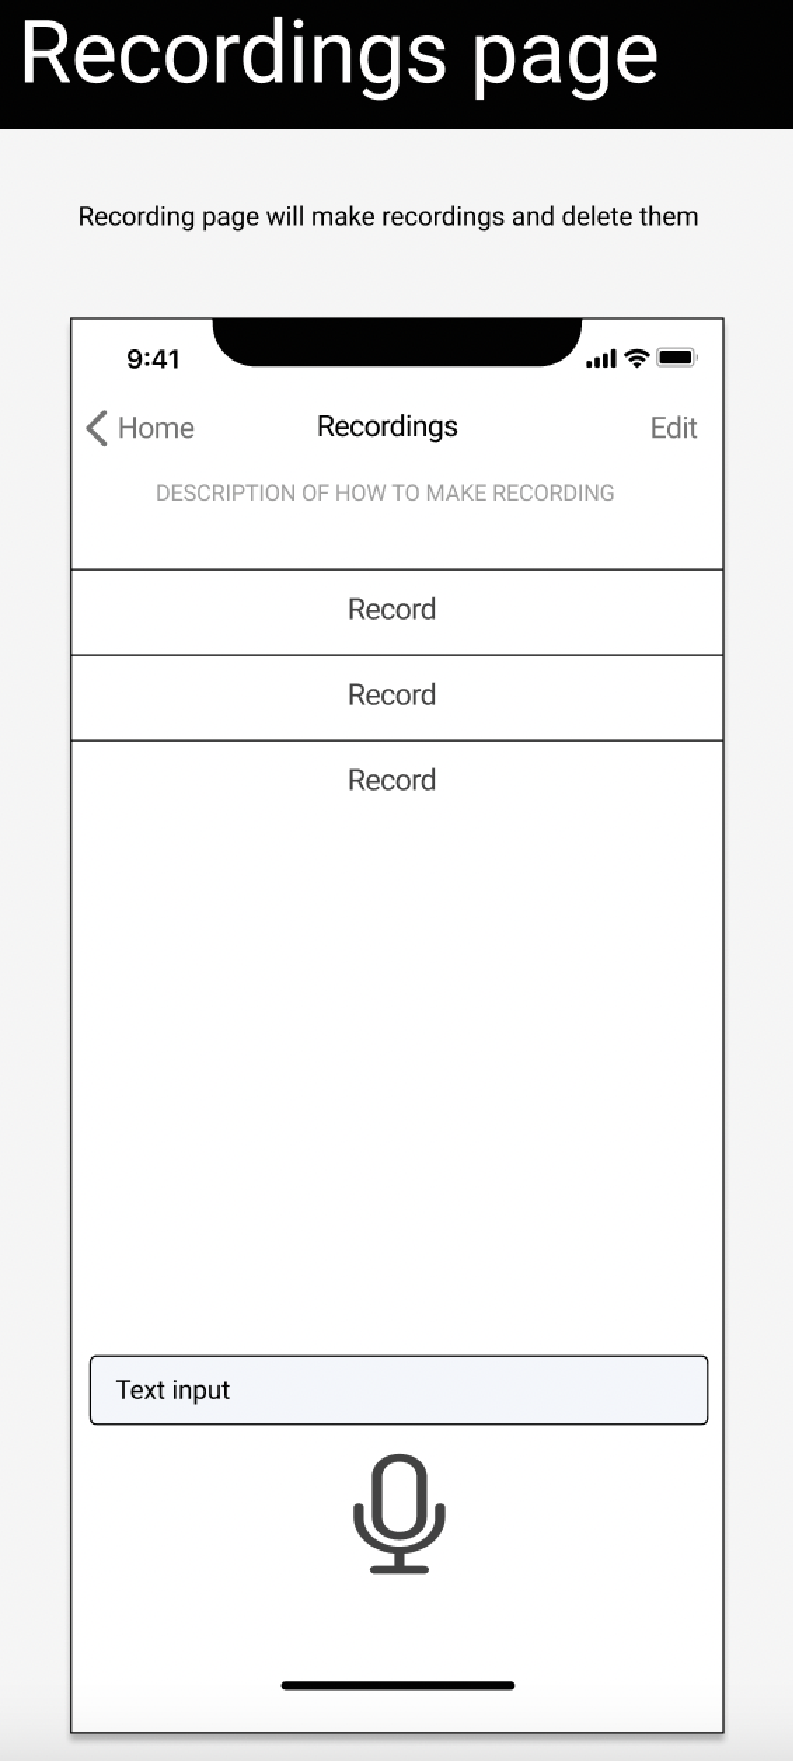
\includegraphics[scale=0.3]{images/RecordingsWireframe.pdf}
        \caption{High fidelity wireframe prototype design for the Recordings view.}
        \label{fig:RecordingsWireframe}
    \end{subfigure} 
    \begin{subfigure}[b]{0.3\textwidth}
        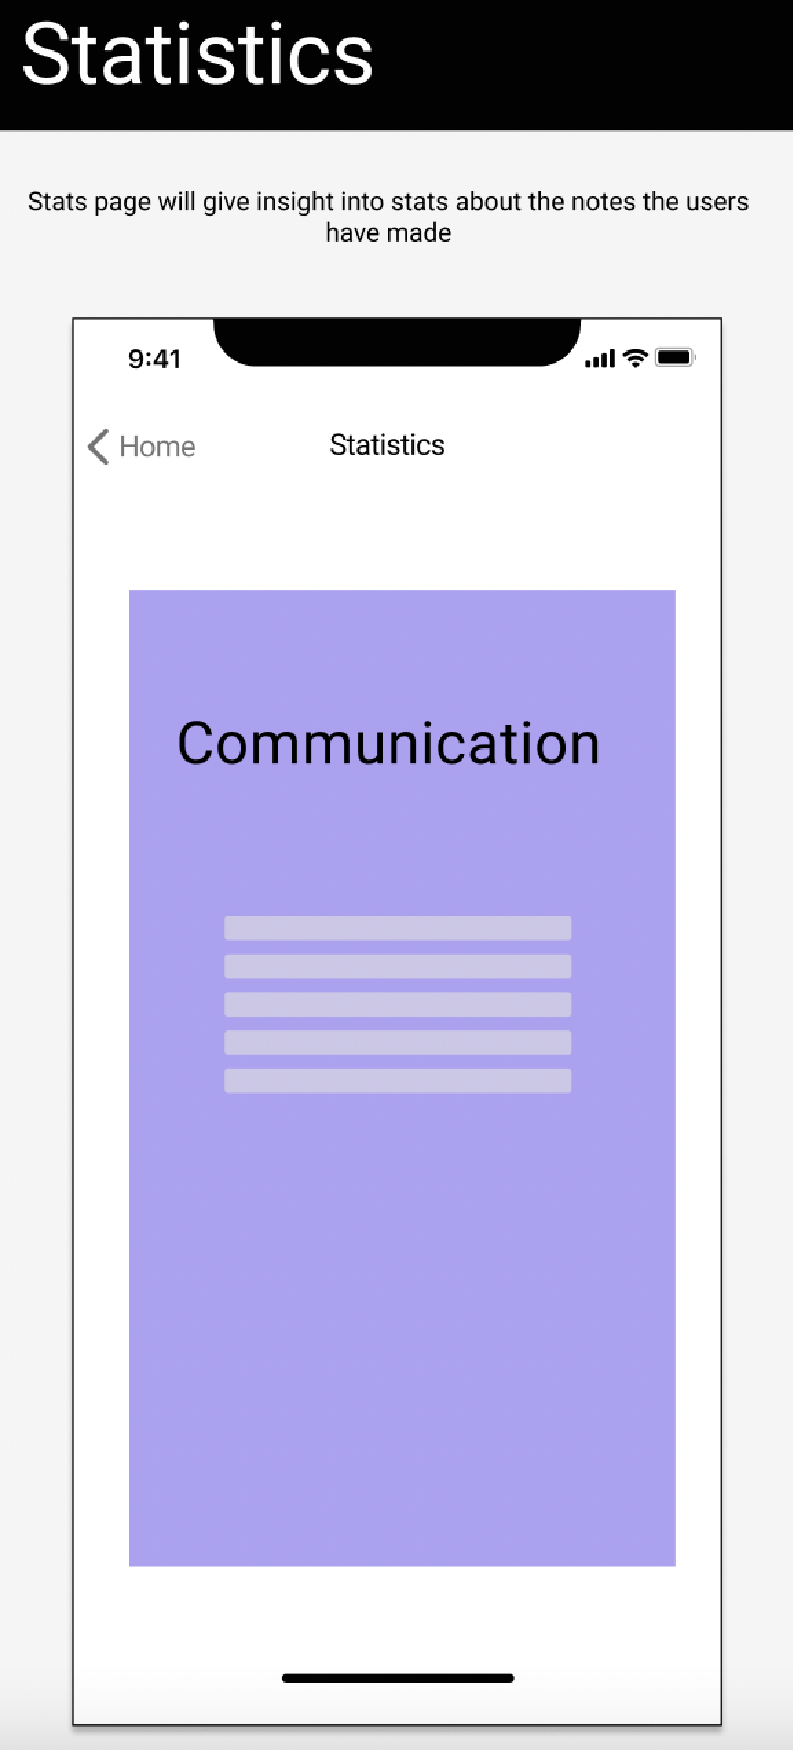
\includegraphics[scale=0.3]{images/StatsWireframe.pdf}
        \caption{High fidelity wireframe prototype design for the Statistics view.}
        \label{fig:StatsWireframe}
    \end{subfigure} 
    \begin{subfigure}[b]{0.3\textwidth}
        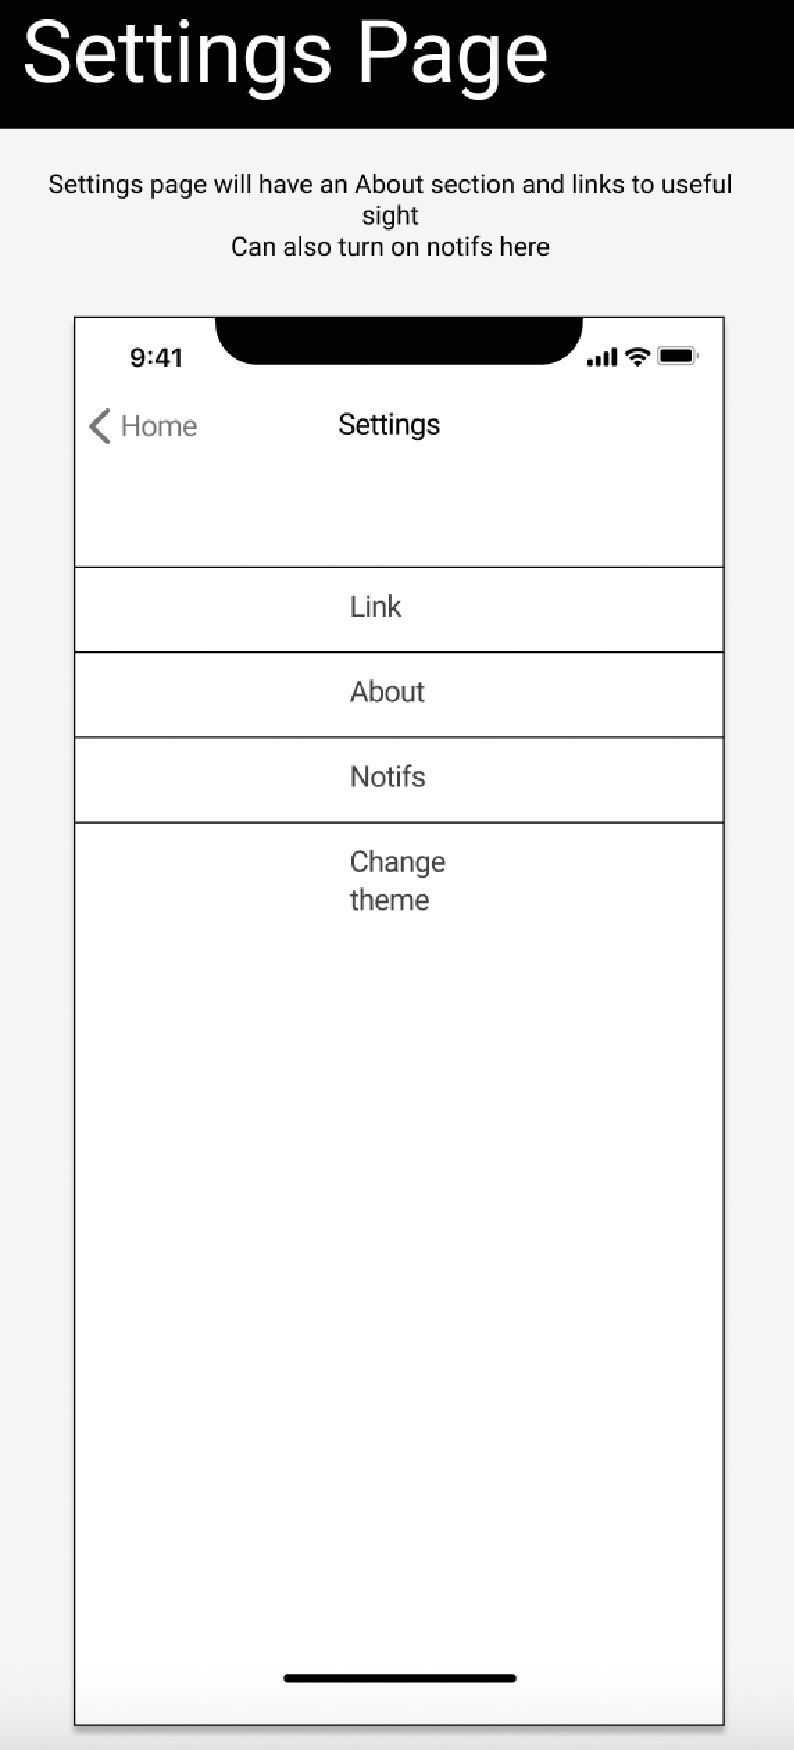
\includegraphics[scale=0.3]{images/SettingsWireframe.pdf}
        \caption{High fidelity wireframe prototype design for the Settings view.}
        \label{fig:SettingsWireframe}
    \end{subfigure}   
    \caption{High-fideility wireframes that were made following the paper prototype designs, smal changes were made to this design for the final product.}
    \label{fig:HighFidWireframes}
\end{figure}

%==================================================================================================================================
%

\section{App Logo} \label{Appendix-AppLogo}

\begin{figure}[H]
    \centering
    
\includegraphics[scale=1]{images/AppLogo.pdf}    
    \caption{This shows the logo created for the mobile app GradReflect.}
    \label{fig:AppLogo} 
\end{figure}

%==================================================================================================================================
%

\section{GradReflect Main Interfaces} \label{Appendix-AppInterfaces}

\begin{figure}[H]
    \centering
    \begin{subfigure}[b]{0.3\textwidth}
        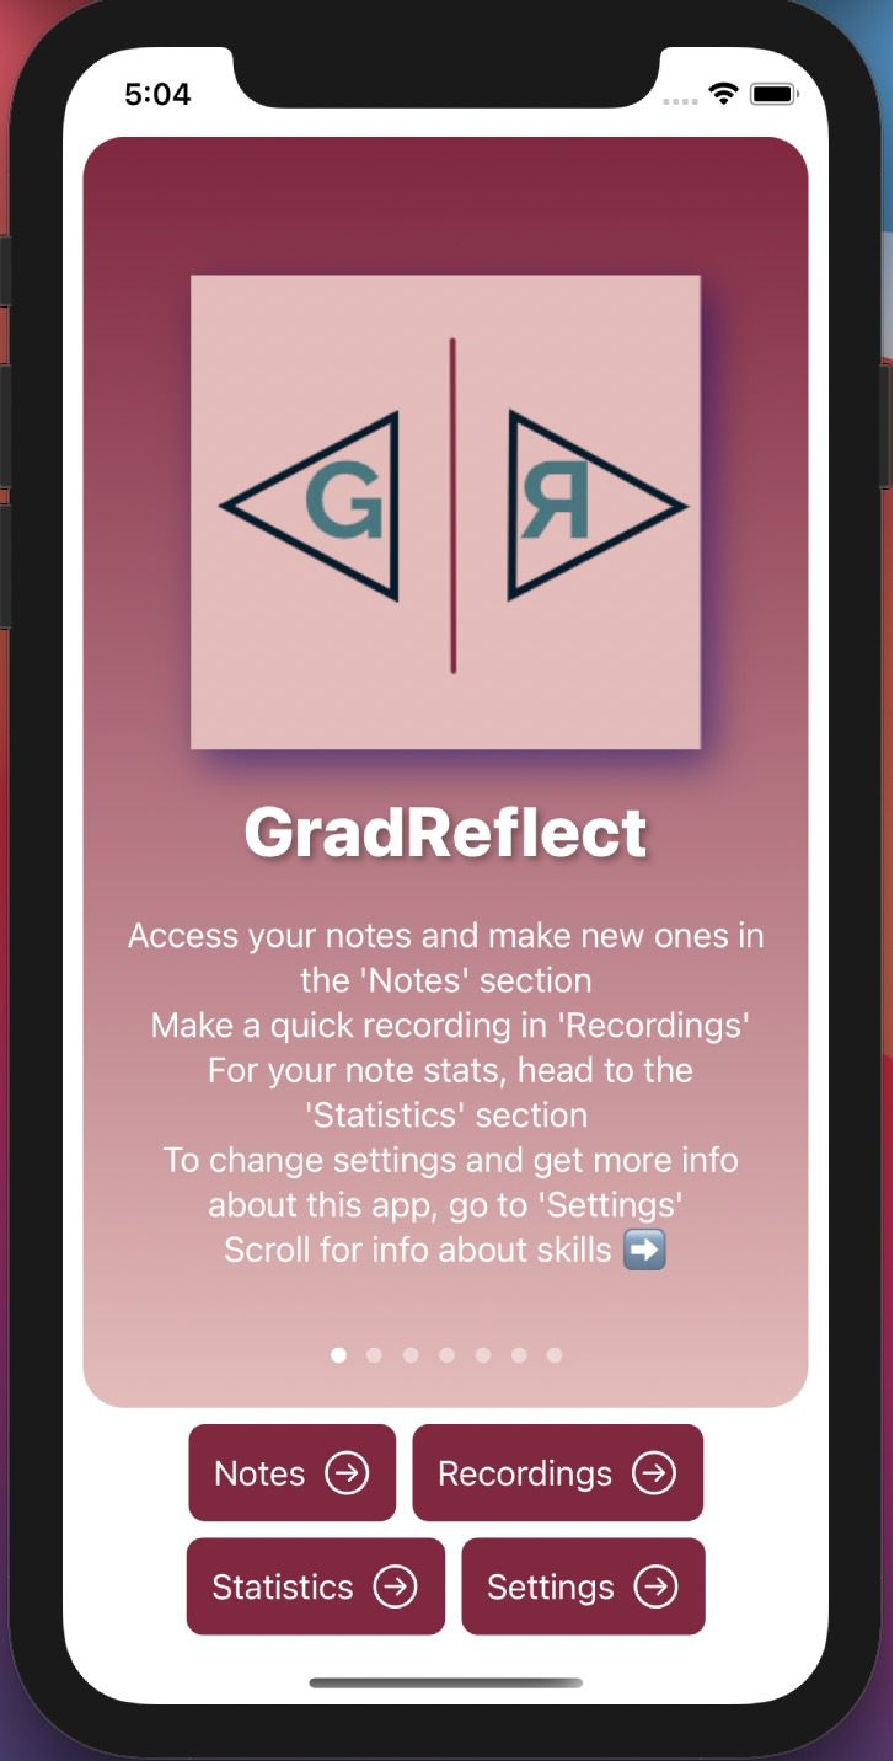
\includegraphics[scale=0.25]{images/appHomeScreen.pdf}
        \caption{Home view}
        \label{fig:appHomeScreen}
    \end{subfigure}
    \begin{subfigure}[b]{0.3\textwidth}
        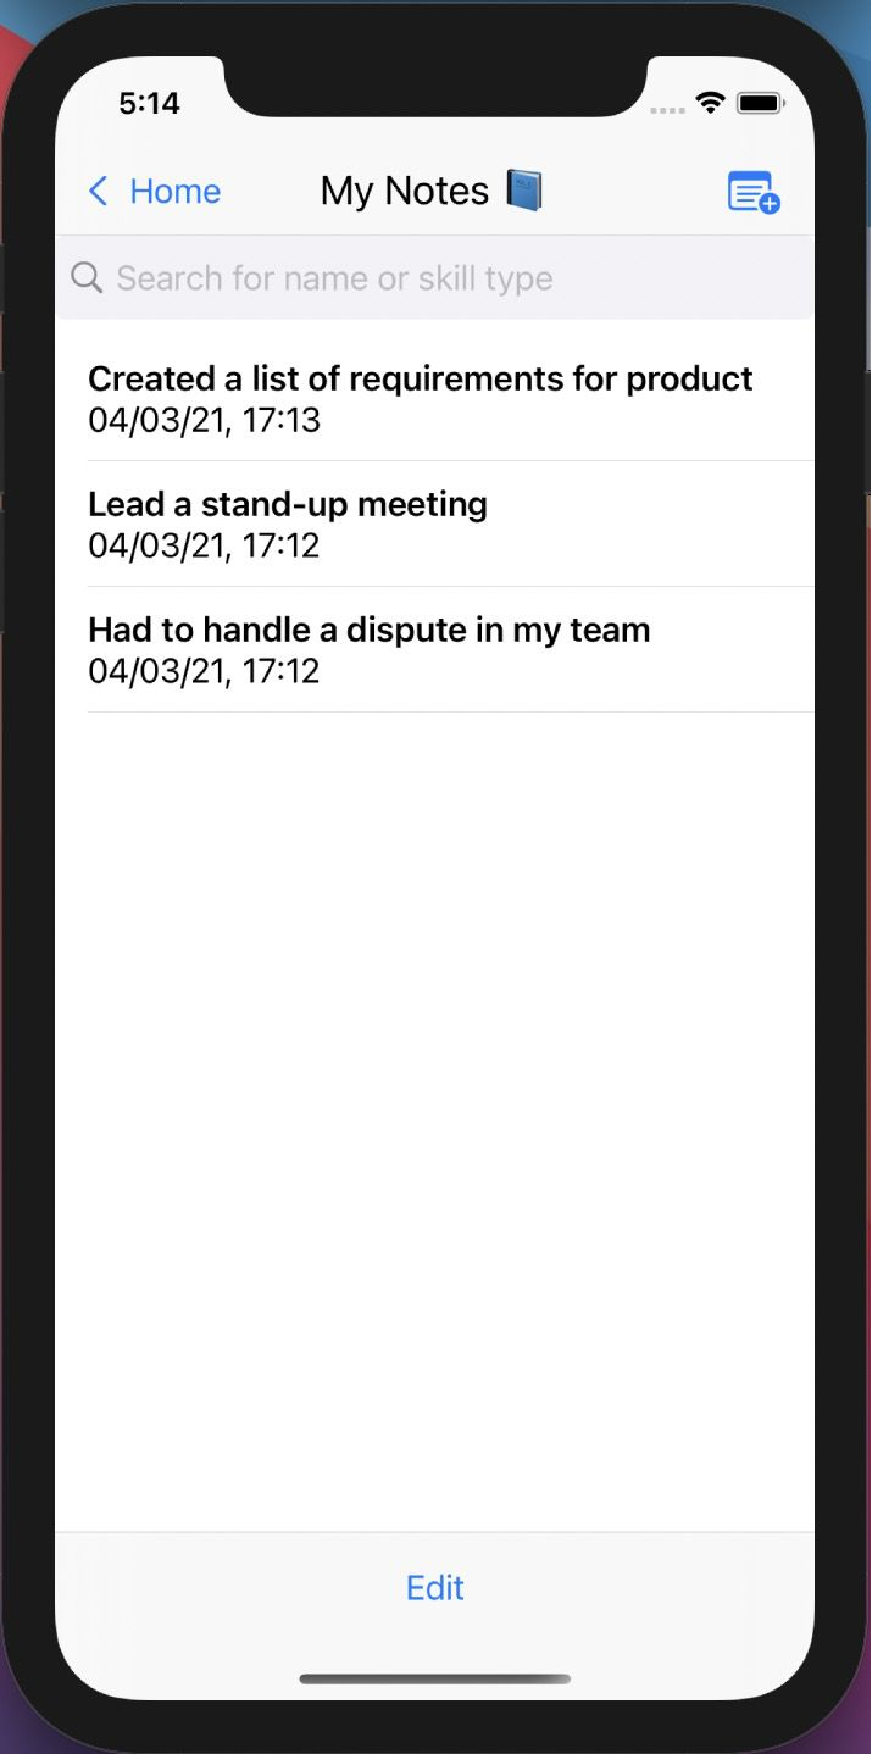
\includegraphics[scale=0.25]{images/appNotesScreen.pdf}
        \caption{Notes view}
        \label{fig:appNotesScreen}
    \end{subfigure}    
    \begin{subfigure}[b]{0.3\textwidth}
        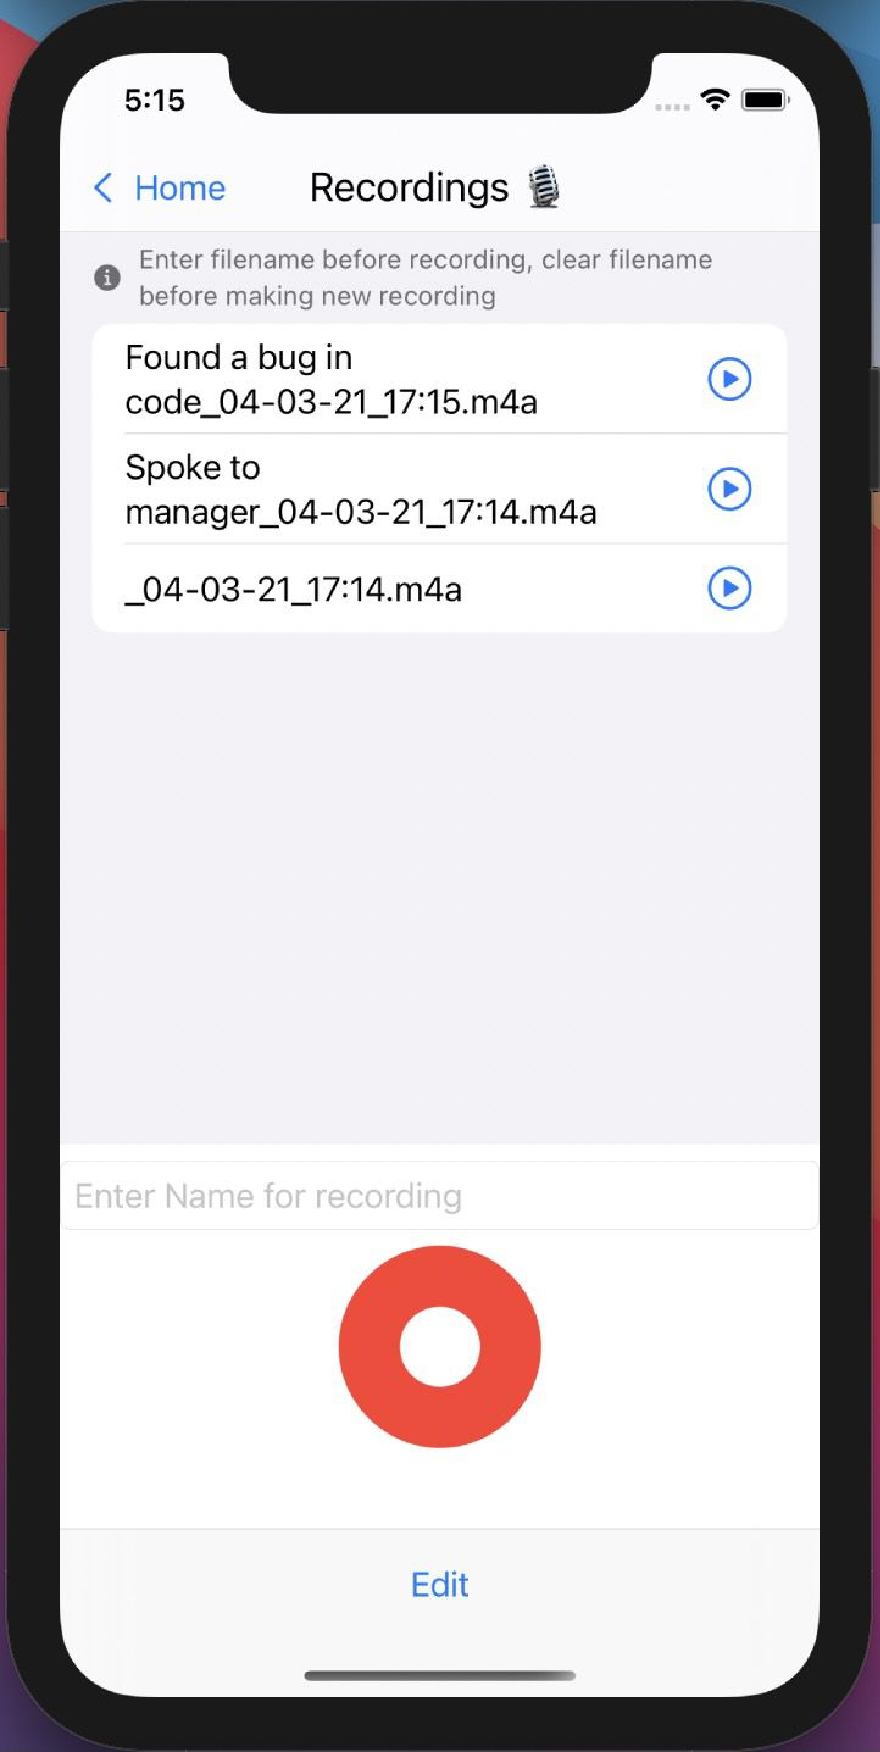
\includegraphics[scale=0.25]{images/appRecordingsScreen.pdf}
        \caption{Notes view}
        \label{fig:appRecordingsScreen}
    \end{subfigure} 
    \begin{subfigure}[b]{0.3\textwidth}
        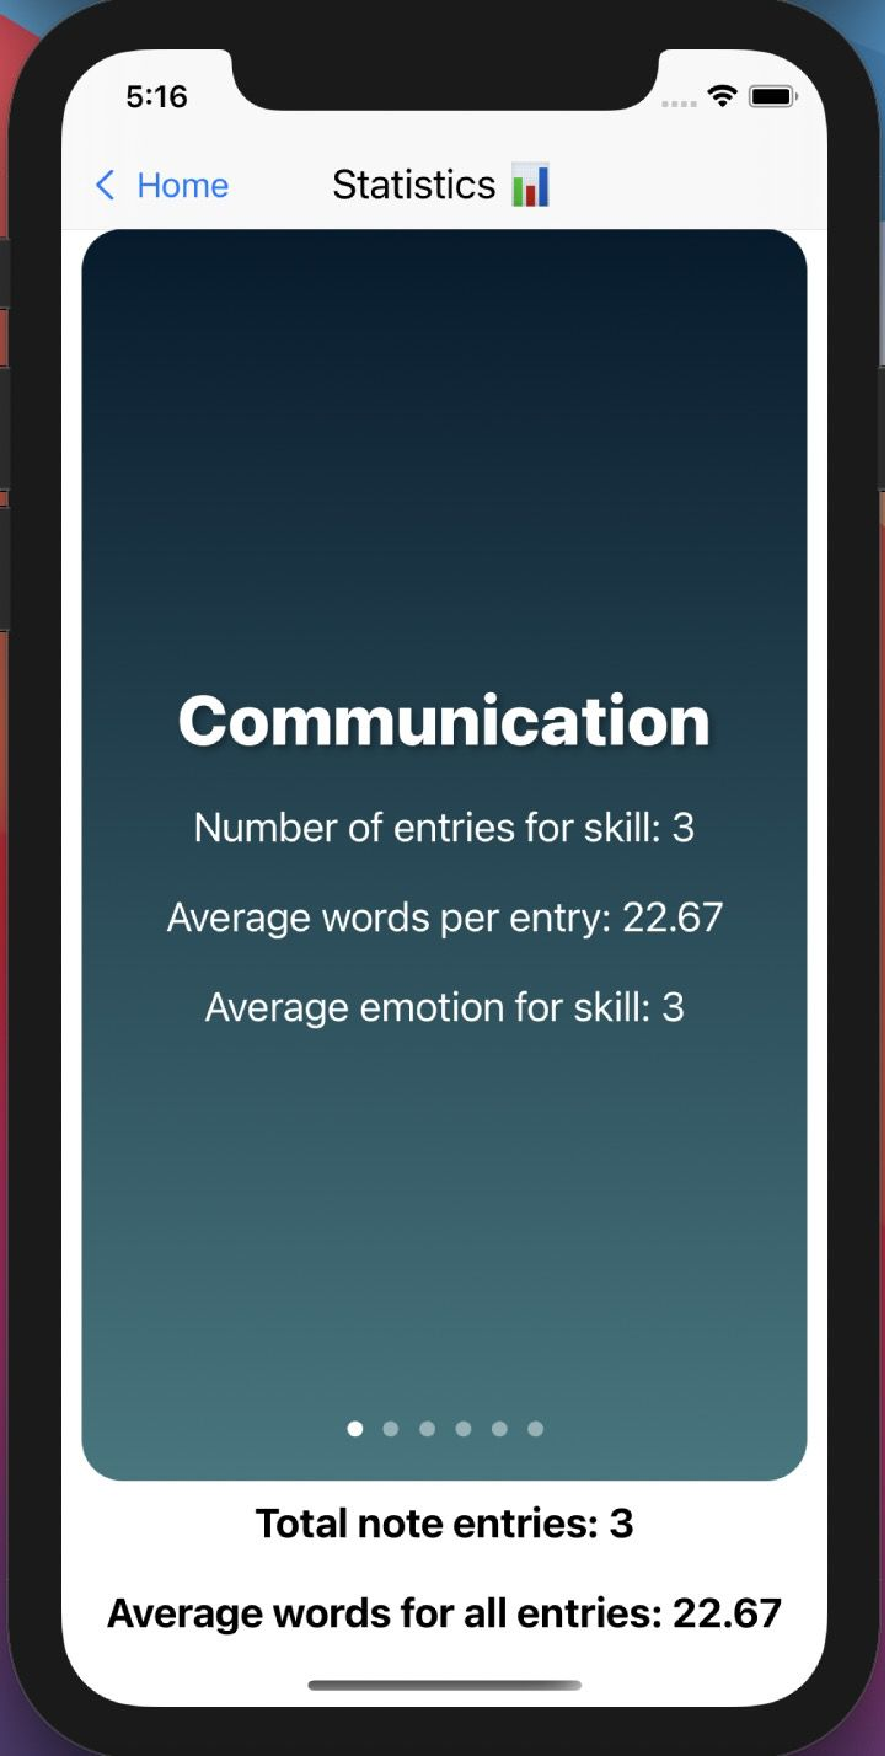
\includegraphics[scale=0.25]{images/appStatScreen.pdf}
        \caption{Statistics view}
        \label{fig:appStatScreen}
    \end{subfigure}  
    \begin{subfigure}[b]{0.3\textwidth}
        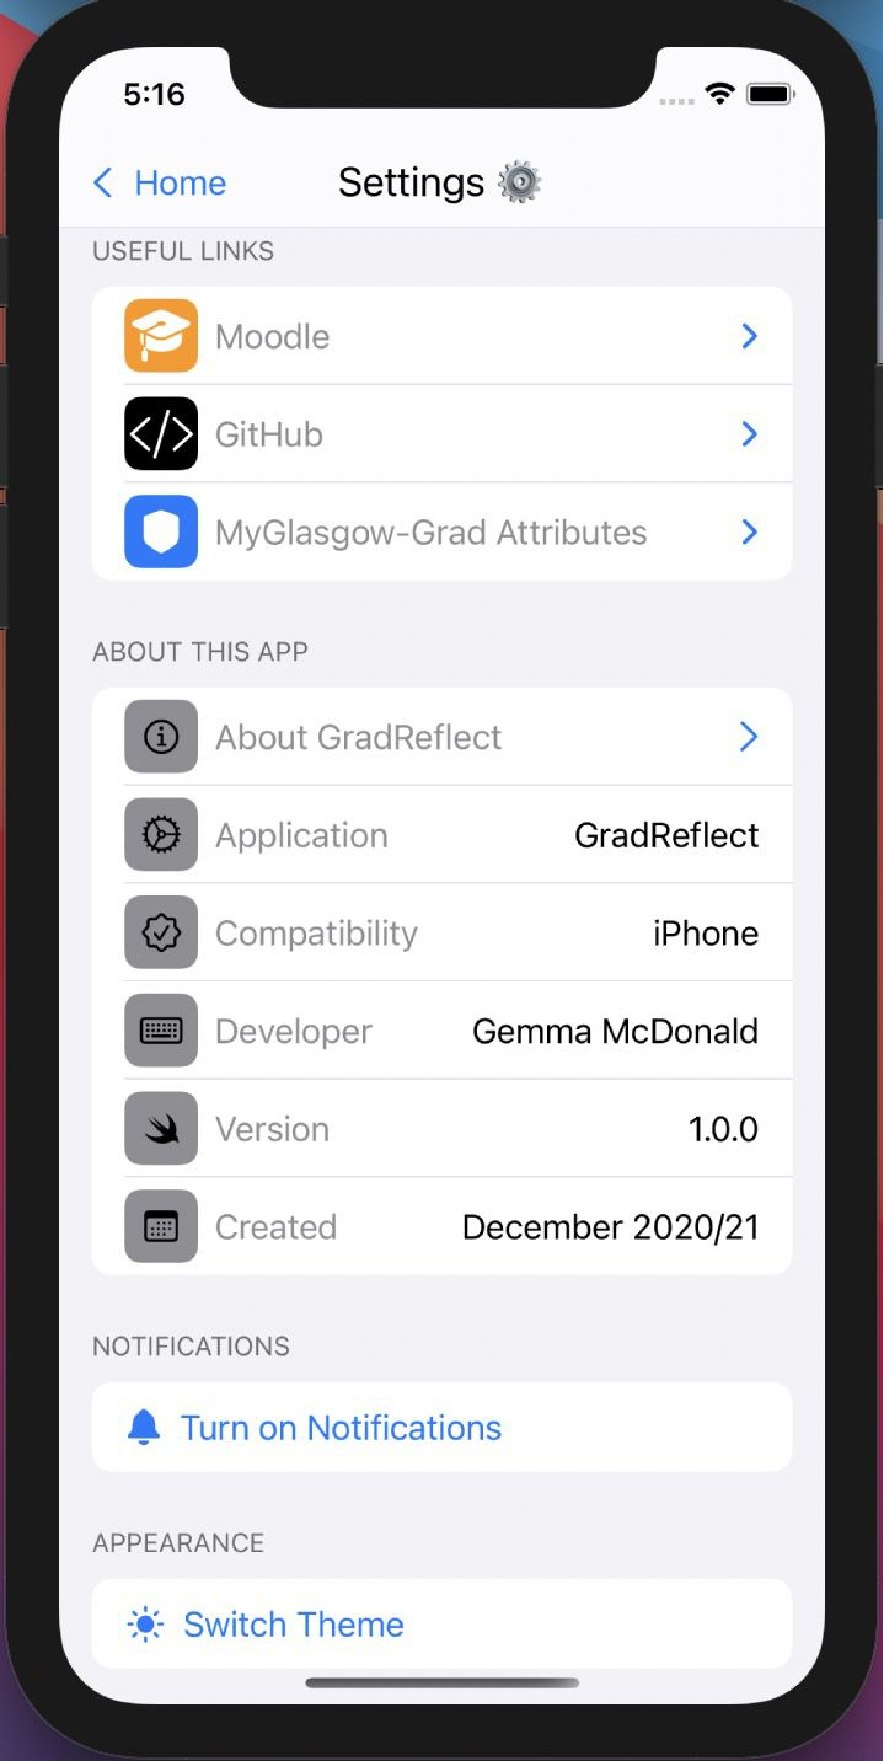
\includegraphics[scale=0.25]{images/appSettingsScreen.pdf}
        \caption{Settings view}
        \label{fig:appSettingsScreen}
    \end{subfigure}  
    \caption{Screenshots showing the main 5 views within the GradReflect app.}
    \label{fig:appMainViews}
\end{figure}

\begin{figure}[H]
    \centering
    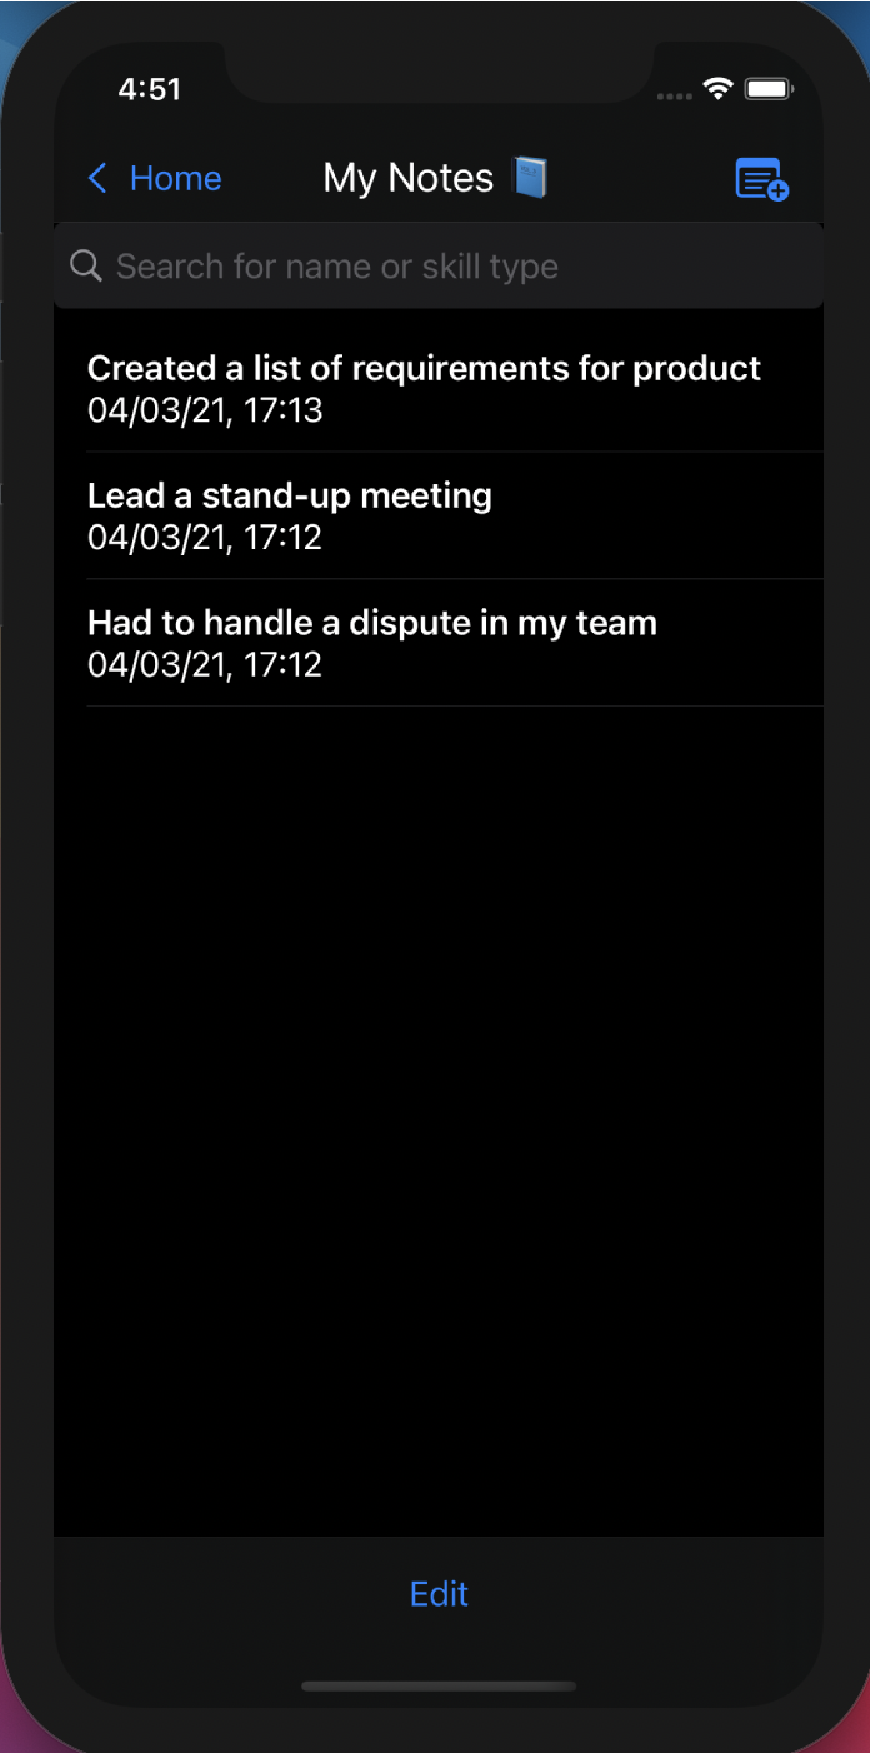
\includegraphics[scale=0.3]{images/DarkMode.pdf}    
    \caption{This screenshot shows the notification the notes view after the user has toggled to dark mode.}
    \label{fig:DarkMode} 
\end{figure}

\begin{figure}[H]
    \centering
    \begin{subfigure}[b]{0.3\textwidth}
        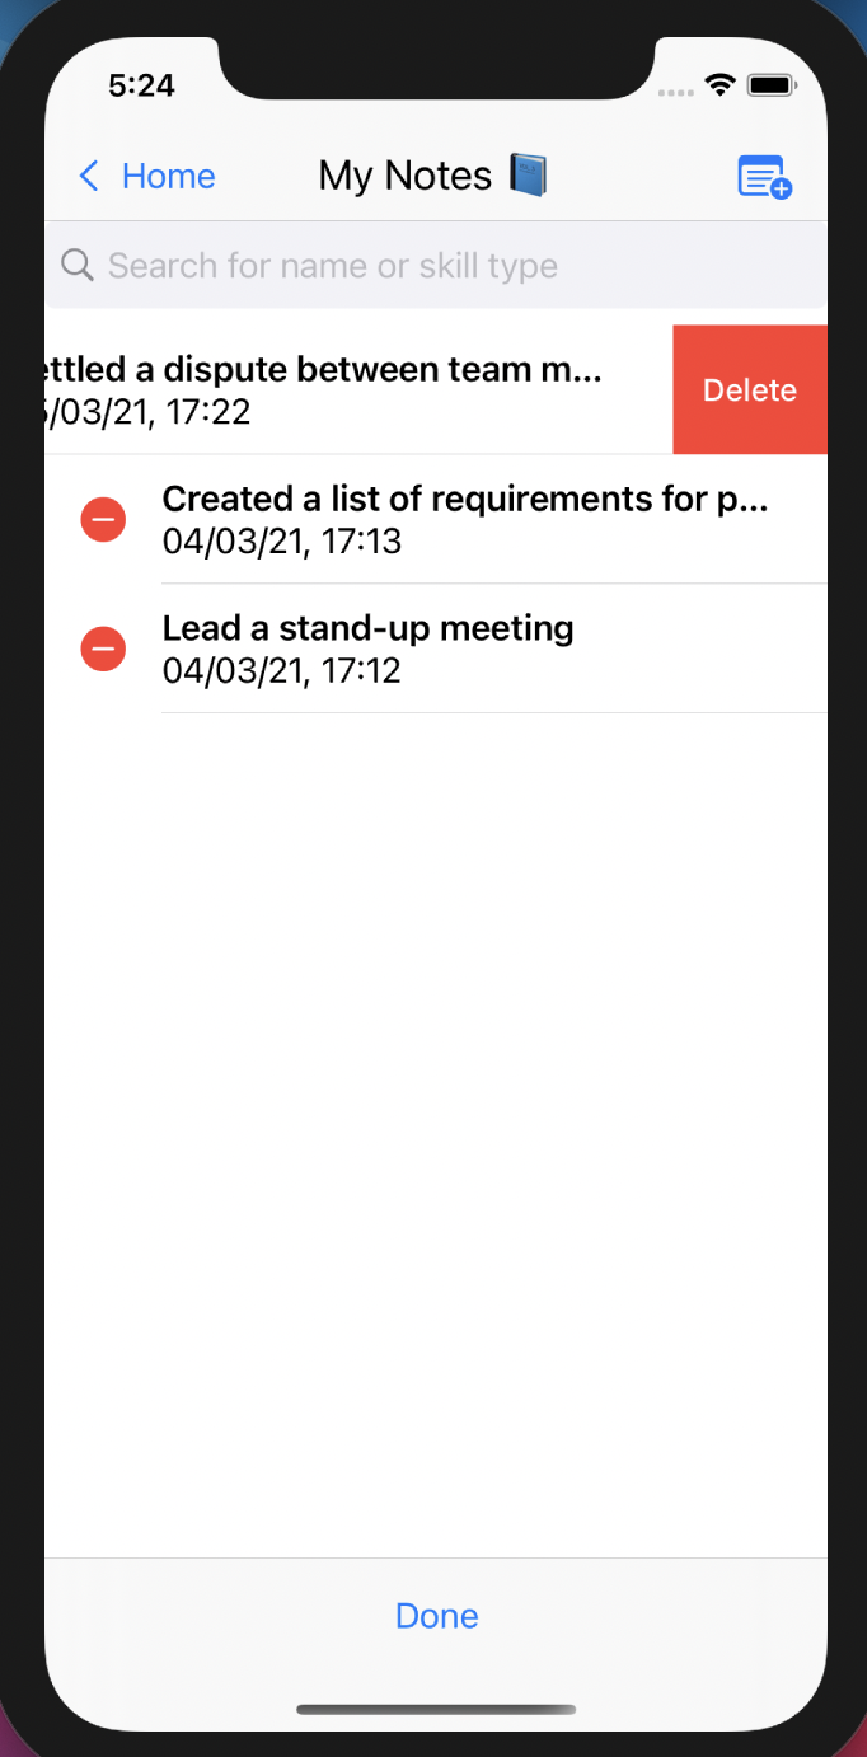
\includegraphics[scale=0.25]{images/DeleteNote.pdf}
        \caption{Delete note.}
        \label{fig:DeleteNote}
    \end{subfigure}
    \begin{subfigure}[b]{0.3\textwidth}
        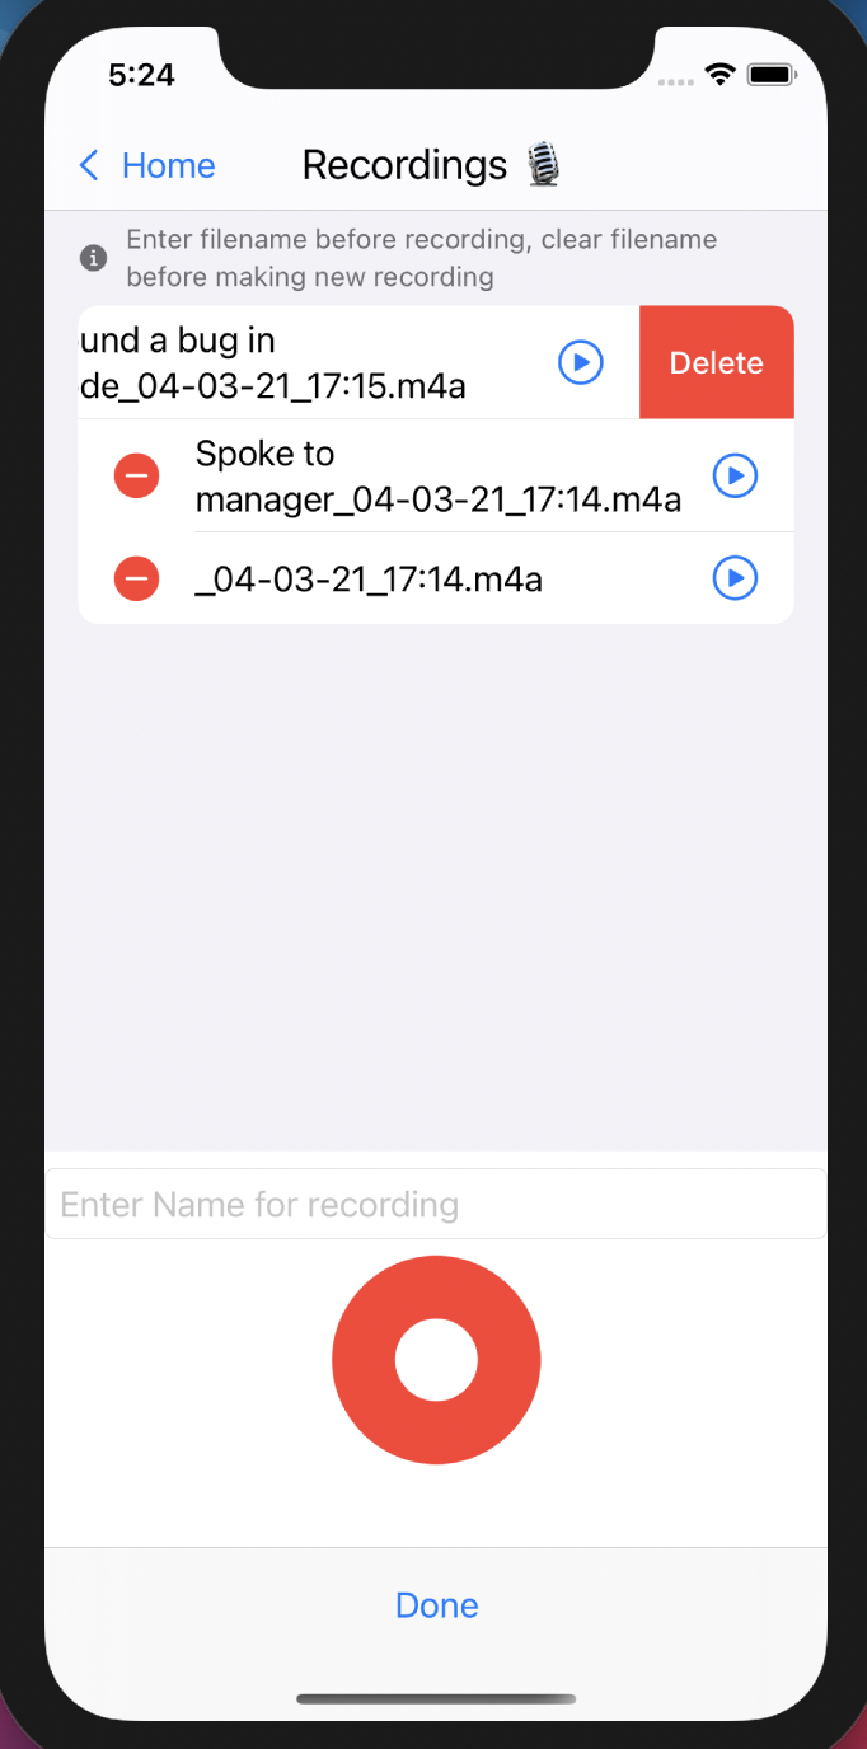
\includegraphics[scale=0.25]{images/DeleteAudio.pdf}
        \caption{Delete audio.}
        \label{fig:DeleteAudio}
    \end{subfigure}   
    \caption{Screenshots showing the edit mode allowing deletion.}
    \label{fig:Deletion}
\end{figure}

\begin{figure}[H]
    \centering
    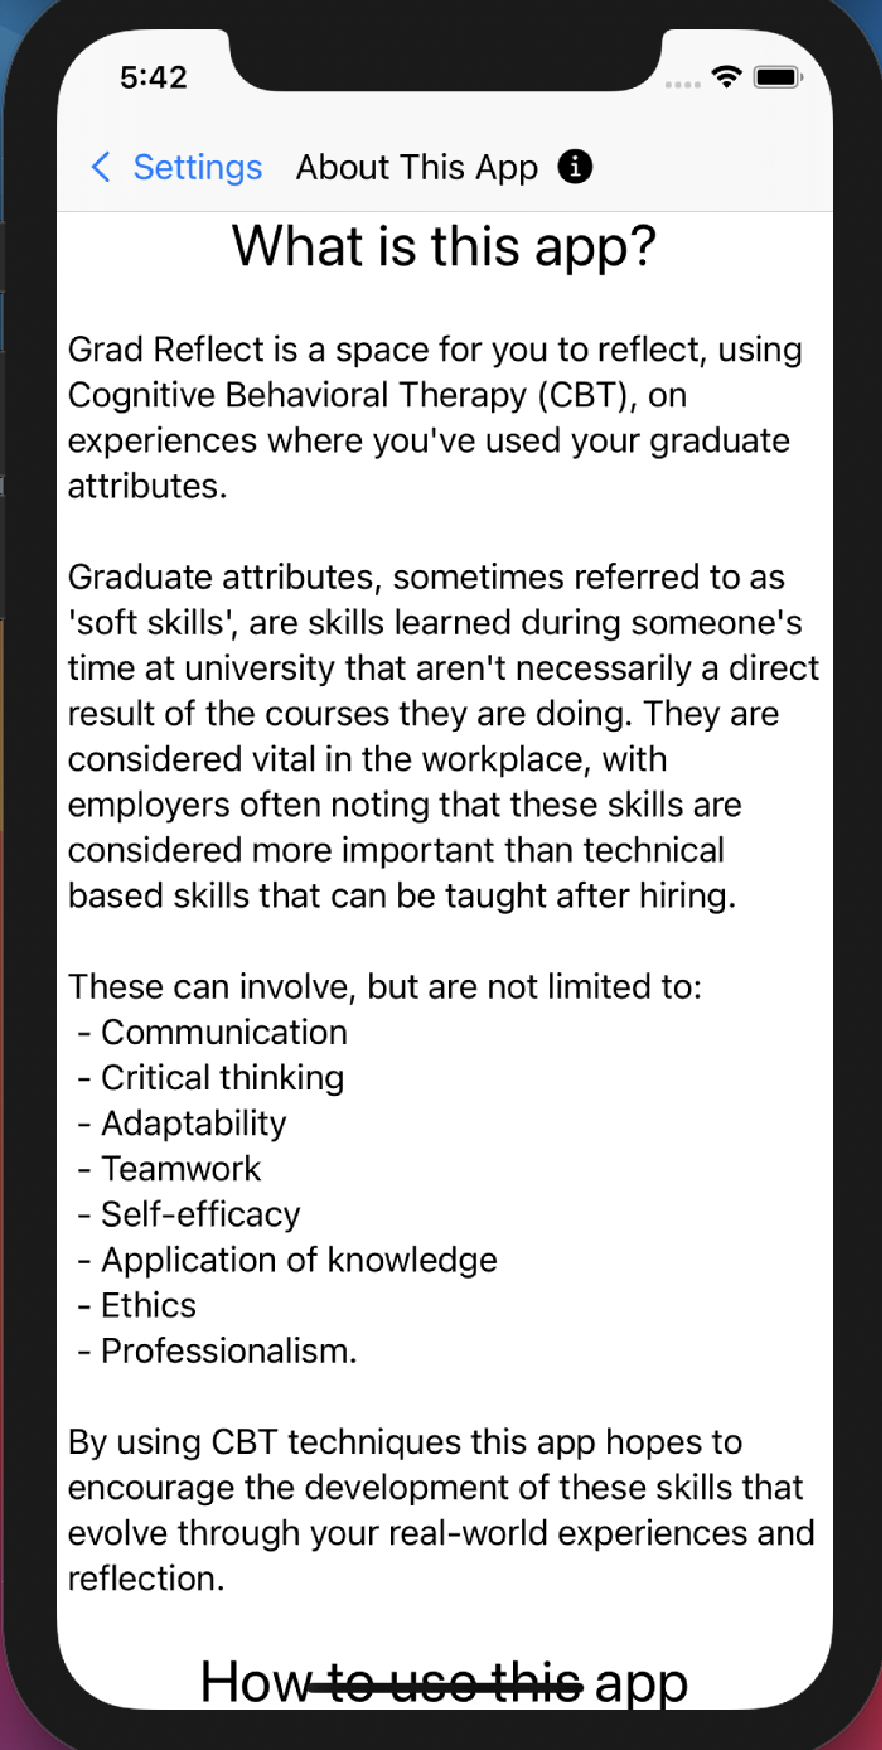
\includegraphics[scale=0.3]{images/AboutApp.pdf}    
    \caption{This screenshot shows the About GradReflect page.}
    \label{fig:AboutApp} 
\end{figure}

%==================================================================================================================================
%

\section{Skill cards}\label{Appendix-SkillCards}

\begin{figure}[H]
    \centering
    \begin{subfigure}[b]{0.3\textwidth}
        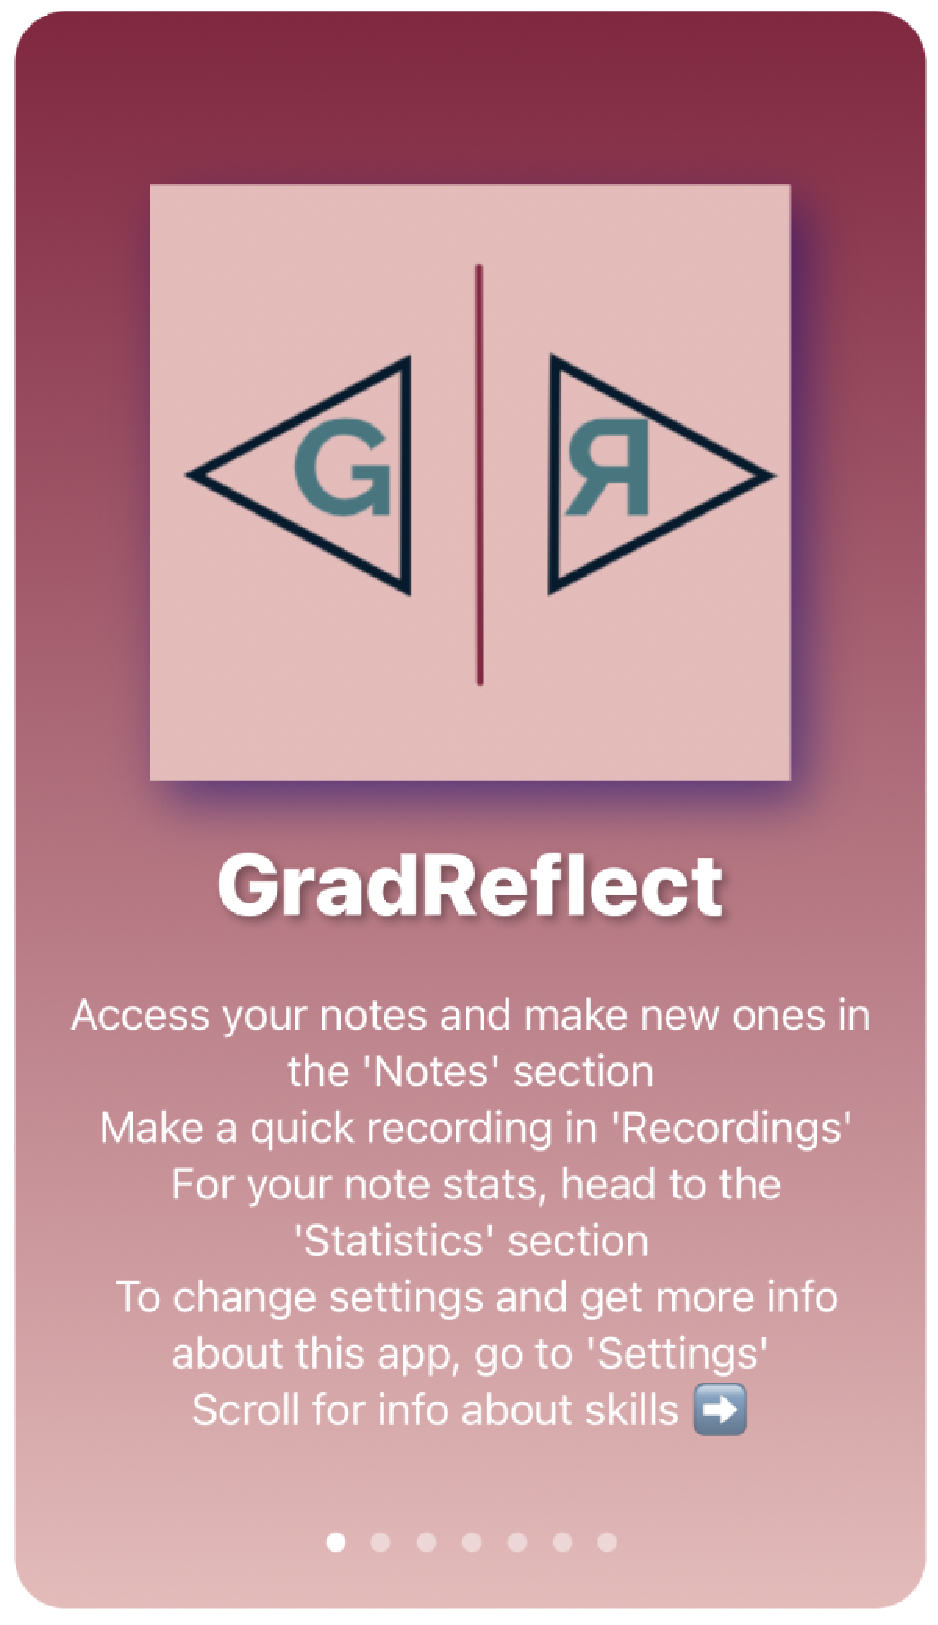
\includegraphics[scale=0.25]{images/HomeCard.pdf}
        \caption{Skill card for Home}
        \label{fig:HomeCard}
    \end{subfigure}
    \begin{subfigure}[b]{0.3\textwidth}
        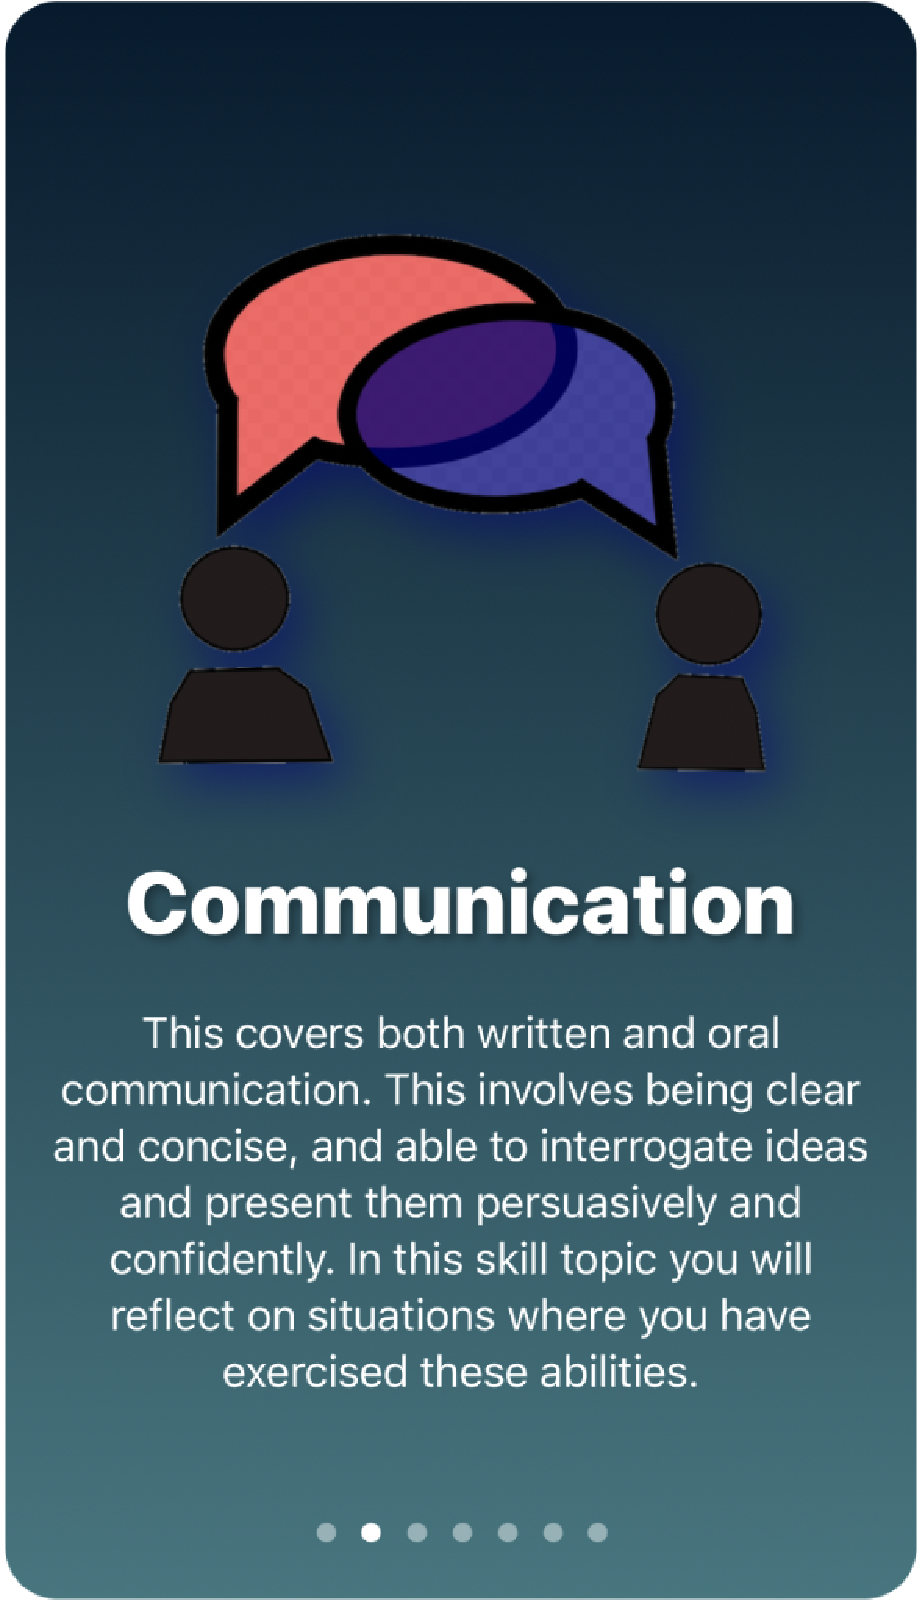
\includegraphics[scale=0.25]{images/CommunicationCard.pdf}
        \caption{Skill card for Communication}
        \label{fig:CommunicationCard}
    \end{subfigure}  
    \begin{subfigure}[b]{0.3\textwidth}
        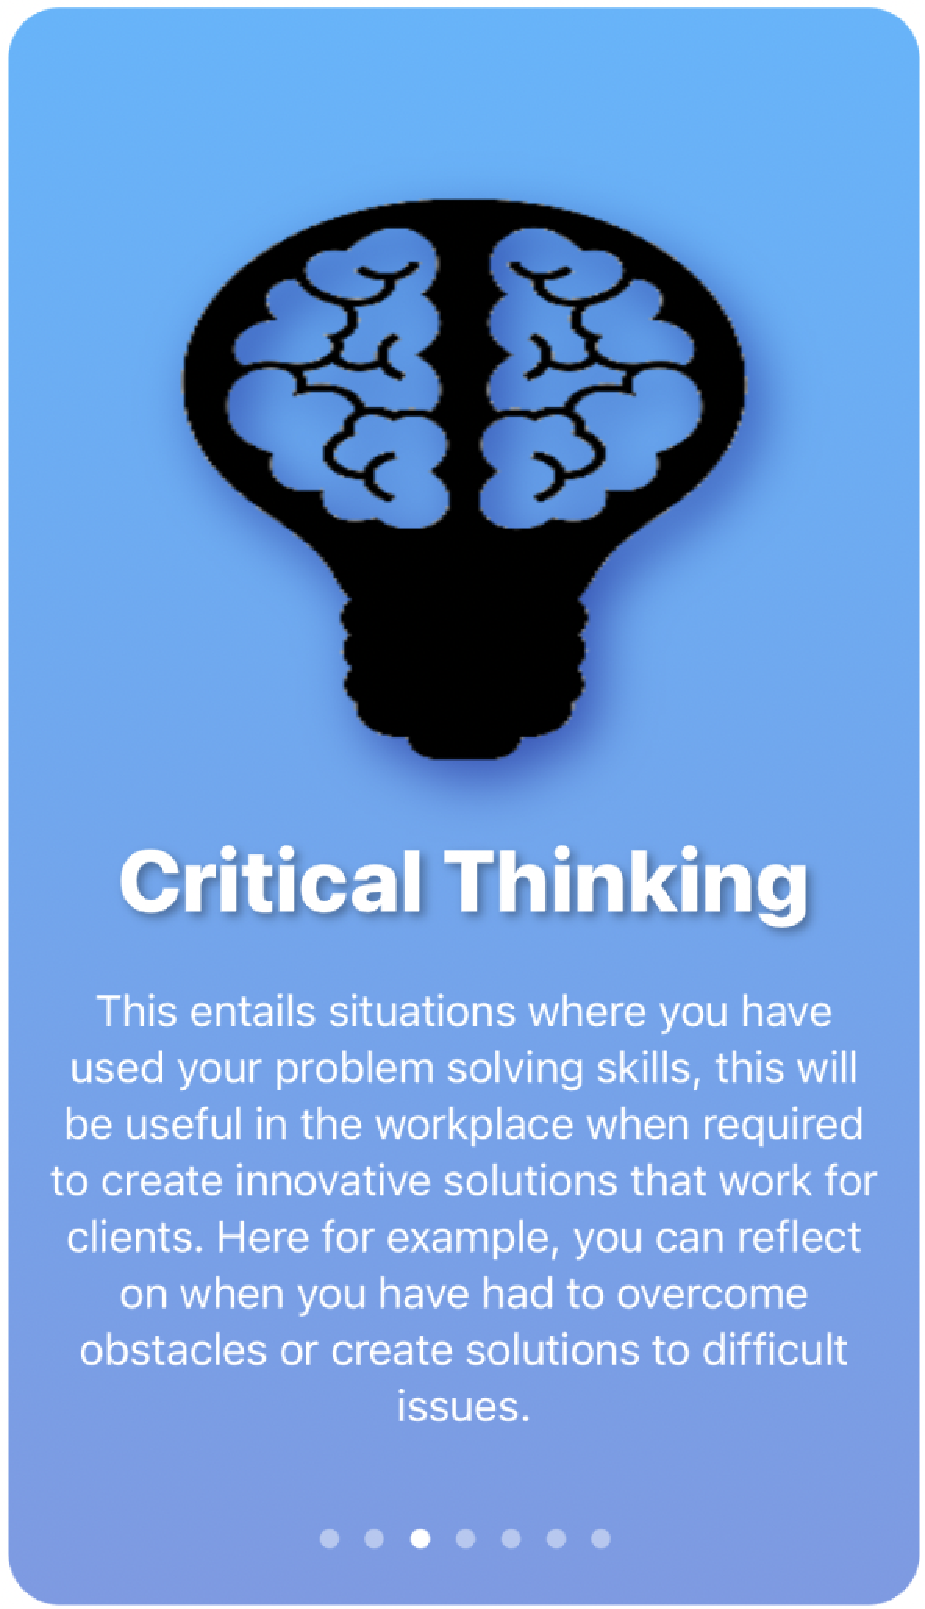
\includegraphics[scale=0.25]{images/CriticalThinkingCard.pdf}
        \caption{Skill card for Critical Thinking}
        \label{fig:CriticalThinkingCard}
    \end{subfigure}
    \begin{subfigure}[b]{0.3\textwidth}
        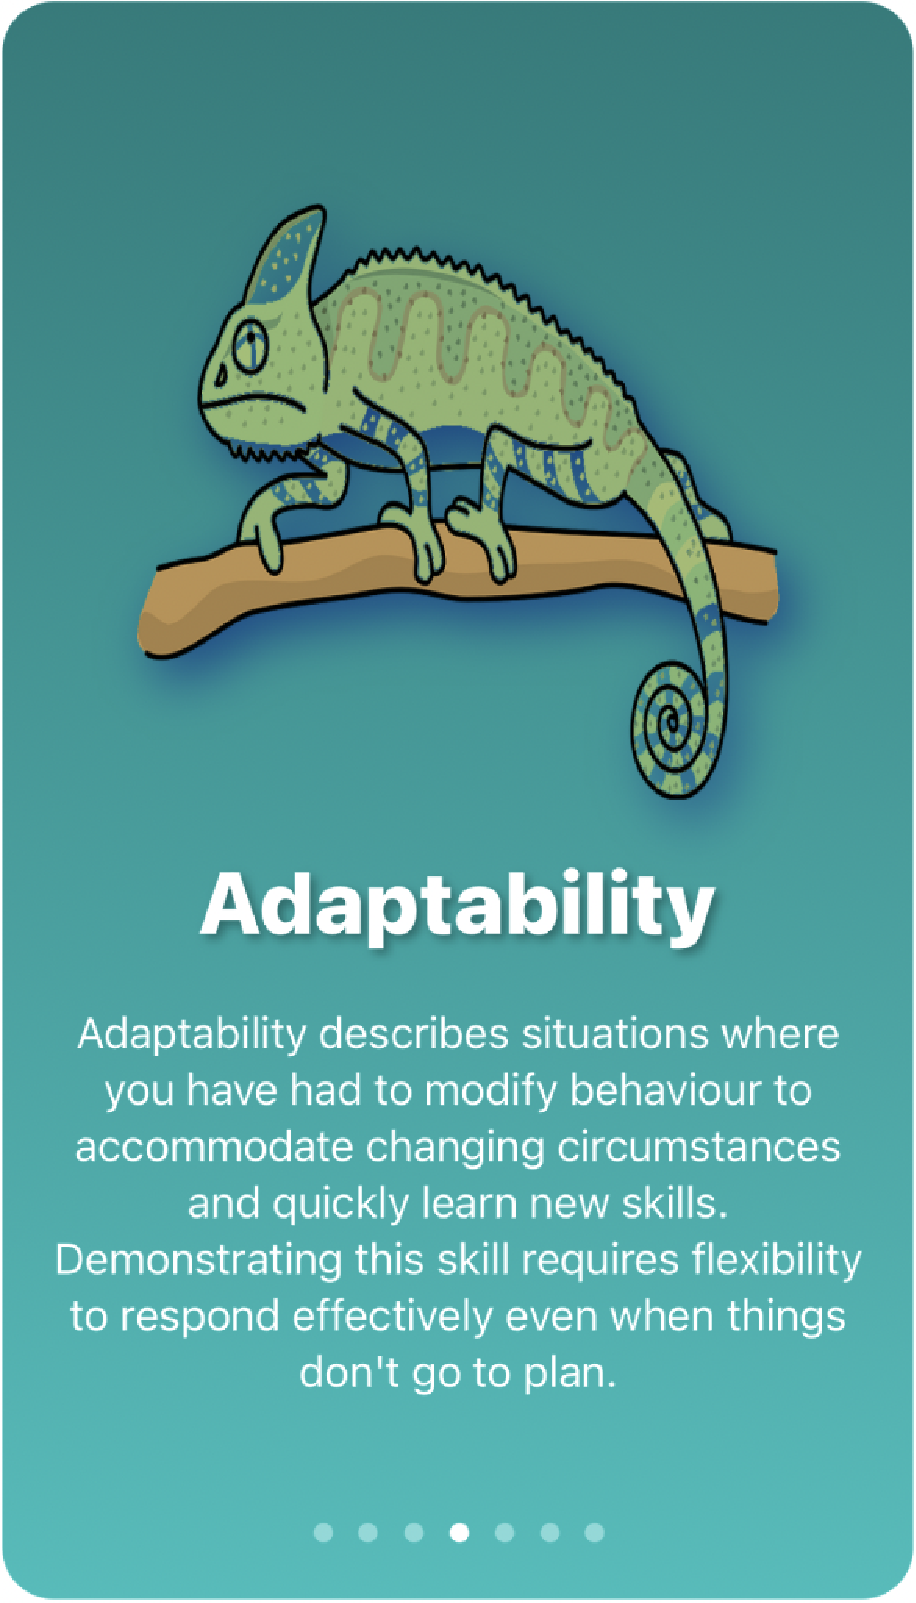
\includegraphics[scale=0.25]{images/AdaptabilityCard.pdf}
        \caption{Skill card for Adaptability}
        \label{fig:AdaptabilityCard}
    \end{subfigure}
    \begin{subfigure}[b]{0.3\textwidth}
        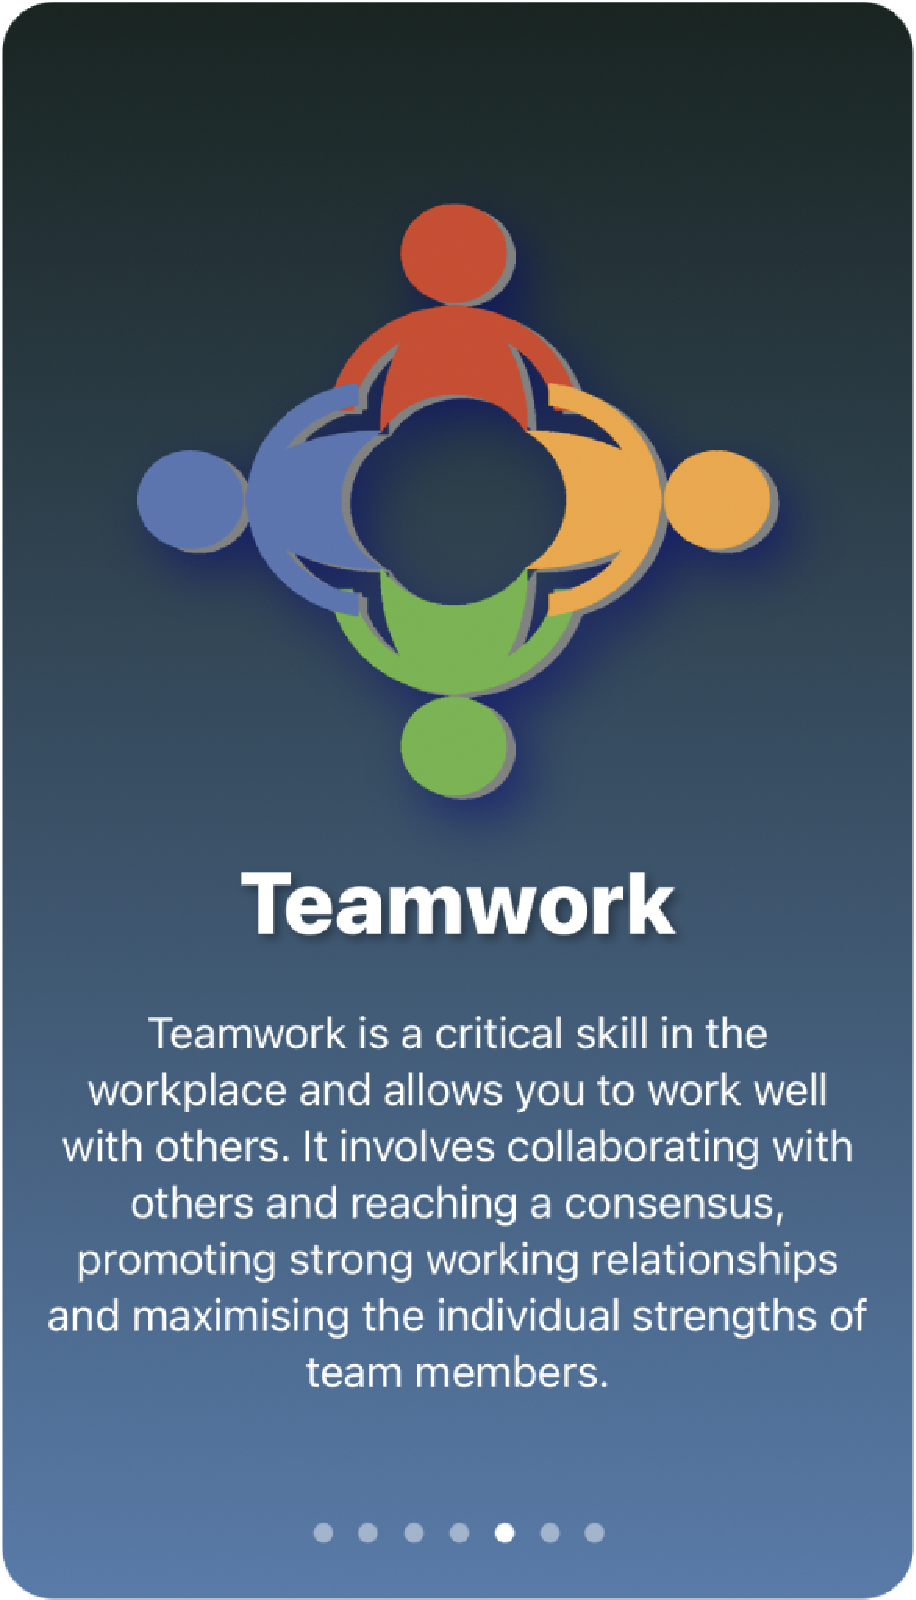
\includegraphics[scale=0.25]{images/TeamworkCard.pdf}
        \caption{Skill card for Teamwork}
        \label{fig:TeamworkCard}
    \end{subfigure}
    \begin{subfigure}[b]{0.3\textwidth}
        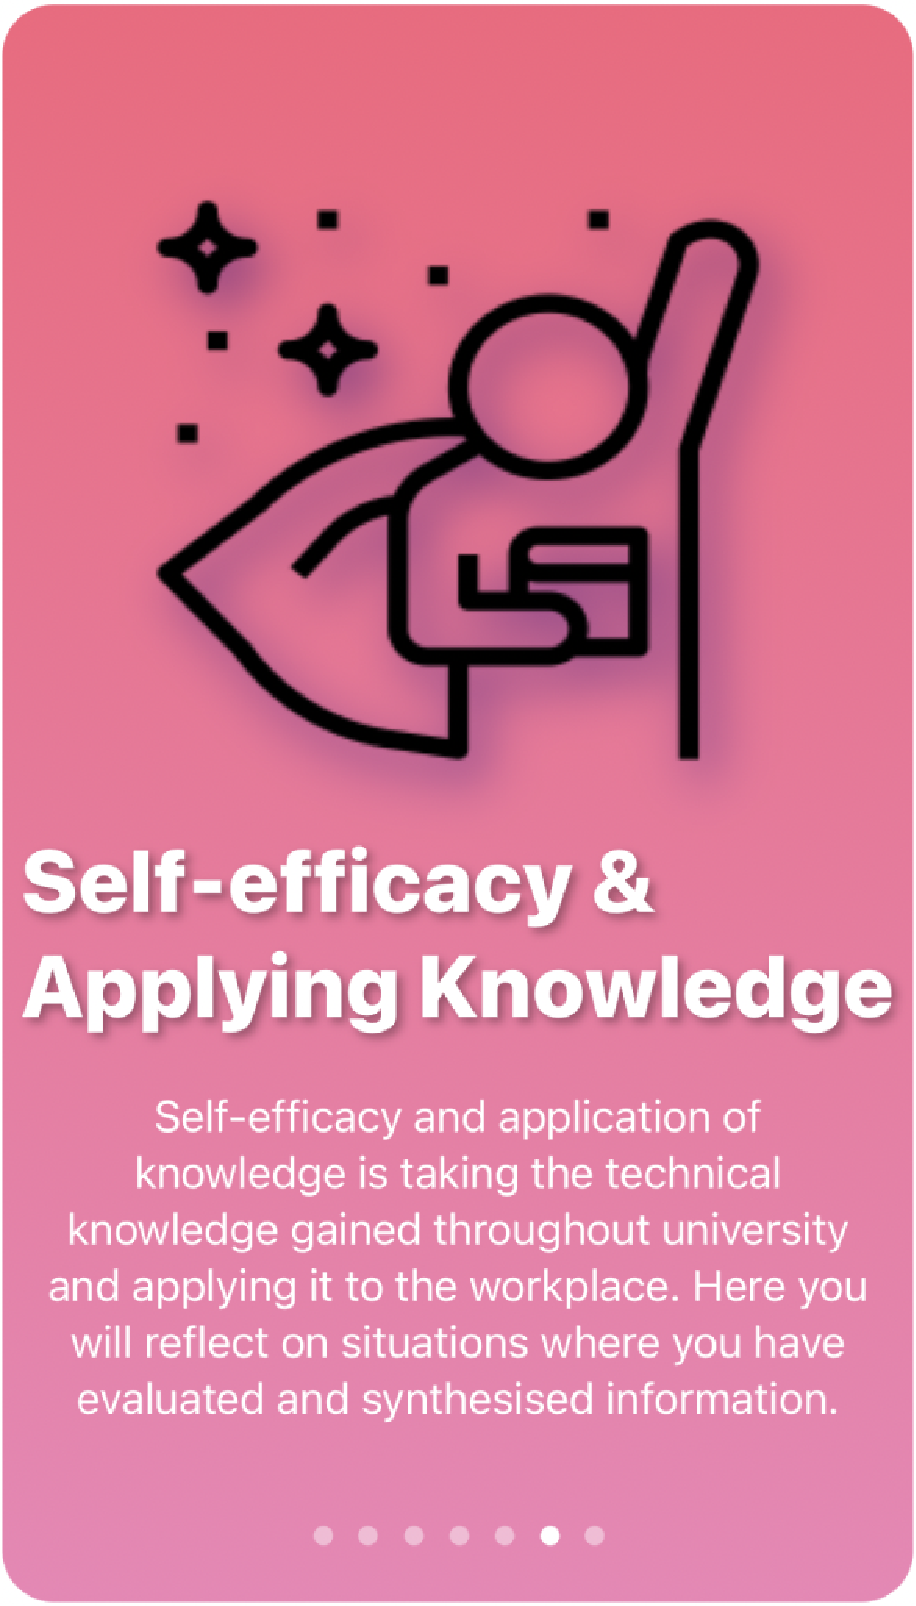
\includegraphics[scale=0.25]{images/SE-AKCard.pdf}
        \caption{Skill card for Self-efficacy and Applying Knowledge}
        \label{fig:SE-AKCard}
    \end{subfigure}
    \begin{subfigure}[b]{0.3\textwidth}
        \includegraphics[scale=0.25]{images/E-ProCard.pdf}
        \caption{Skill card for Ethics and Professionalism}
        \label{fig:E-ProCard}
    \end{subfigure} 
    \caption{Screenshots showing the skill cards in the Home View of the app GradReflect.}
    \label{fig:AllSkillCards}
\end{figure}



%==================================================================================================================================
%

\section{User Evaluations} \label{Appendix-UserEvals}

\subsection{Introduction Script}

SCHOOL OF COMPUTING SCIENCE - UNIVERSITY OF GLASGOW

The aim of this experiment is to investigate the usability of the GradReflect mobile application.

We cannot get an understanding of this without participation from the people who would be likely to use this application if it were to be released for general use by the public.

I will give you some time to explore and familiarise yourself with the application, before asking you to complete a set of tasks to test each aspect of the application. I will be observing you as you complete these tasks. Following this you will be sent a Google Form to complete a usability survey.

The answers will be collected and analysed.

Please ask questions if you need to, I will be available during and after the survey by email.

Please remember that this is to evaluate the mobile application, and is in no way an evaluation on you, the participant.

You are able to withdraw from the survey at any time.

Do you agree to take part in this evaluation?

Do you have any questions before we start?


\subsection{Debrief Script}

The main aim of this experiment was to gain an insight into the usability of the GradReflect app.

However, I was particularly looking to see if the reflection was simple to complete and if navigating through the app was clear and easy, as well as finding out if you would be likely to continue using this app in the future.

Do you have any comments or questions about the experiment?

I am now going to send you the link to the survey form to answer some questions on your experience.

Please take a note of my email address, and please let me know if you have any further questions about this experiment.

Gemma McDonald 2306631m@student.gla.ac.uk

Thank you for your help.


\subsection{Task List} \label{Appendix-taskList}

\textbf{List of tasks to ask an evaluation participant to do}

Users will first be given 5-10 minutes to explore the app and try out different features, and familiarise themselves with the general layout of the app

\textbf{Home page}

\begin{itemize}
    \item Review the description of each skill on the Home page section Settings page
    \item Navigate to the settings page
    \item Attempt to follow each of the useful links to the sites, returning each time to the app
    \item Read the About GradReflect page
    \item Turn on notifications and close the app to wait for the incoming notification and return to the app
    \item Change the theme of the app and navigate to anywhere in the app to view the changes to the interface
\end{itemize}

\textbf{Notes page}

\begin{itemize}
    \item Navigate to the notes section and create a note named "My first note", in which you select the skill "Teamwork" and describe an example where you worked in a team. You may use available helper '?' buttons if you are unsure how to answer a question. Save this note.
    \item Try to review the answers on a note
    \item Attempt to create and save a note with no name.
    \item Cancel creating this note
    \item Search for the title or specified skill of your note
\end{itemize}

\textbf{Stats page}

\begin{itemize}
    \item Navigate to the statistics section and review the stats based on notes you have created
    \item Return to the notes section and delete the note you created a moment ago
\end{itemize}

\textbf{Recordings page}

\begin{itemize}
    \item Navigate to the recordings section
    \item Name and create a recording
    \item Create a recording without giving it a name.
    \item Playback your notes
    \item Delete one of the recordings you created
    \item Return to homepage
\end{itemize}

\subsection{Survey Questions} \label{Appendix-EvalSurveyQuestions}

\textbf{Part 1}

\begin{enumerate}
    \item The app always made it clear what the system was currently doing. I could always see where I am on the page and feedback was provided immediately.
    \item Comments on the above question
    \item The app's wording was easy to understand. I didn't need to look up any terminology, as all expert language was explained well.
    \item Comments on the above question
    \item I never got stuck and felt frustrated doing a certain action and always knew how to back out of an action. I always felt in control of the system.
    \item Comments on the above question
    \item The app was consistent. I found it easy to use, and the layout was similar to apps I have used before.
    \item Comments on the above question
    \item I did not spot any errors or problems in the app. Any error messages were easy to understand and helped me correct my mistake.
    \item Comments on the above question
    \item The app always was easy to understand. I never had to scroll back to understand what the app wants from me. Buttons were easily found.
    \item Comments on the above question
    \item I could customise the app to my own personal preferences by doing searches and display options. Once I knew how to use the app I could navigate through very quickly.
    \item Comments on the above question
    \item The app only contained essential items with no major distractions on the app. The functionality of the app was the main focus.
    \item Comments on the above question
    \item Error messages I received were plain language and showed me how to correct the problem.
    \item Comments on the above question
    \item The app had extra descriptions and help of how to use it if and advice was required.
    \item Comments on the above question
\end{enumerate}

\textbf{Part 2}

\begin{enumerate}
    \item How easy did you find the application to reflect?
    \item Was there enough assistance to aid in your reflection? I.e. - the '?' buttons and the 'About GradReflect' page
    \item Can you give insight into why you chose your previous answer?
    \item Were you able to quickly make a note of how and when you have used a skill in university/workplace etc?
    \item Can you give insight into why you chose your previous answer?
    \item Would you continue to use this app?
    \item Can you give insight into why you chose the previous answer?
    \item Did you find the ability to make voice recordings useful?
    \item Can you give insight into why you chose your previous answer?
    \item Did you find the statistics page useful?
    \item Can you give insight into why you chose your previous answer?
    \item Are there any changes you would want made to the application? E.g. improvements or new features
\end{enumerate}


\subsection{Survey Part 1-Likert scale responses} \label{Appendix-surveyP1-individualHeuristicGraphs}

\begin{figure}[H]
    \begin{centering}
    \includegraphics[scale=0.5]{images/heuristic1.pdf}
    \caption{Breakdown of the responses to the question "The app always made it clear what the system was currently doing. I could always see where I am on the page and feedback was provided immediately."}
    \label{fig: heuristic1}
    \end{centering}
\end{figure}

\begin{figure}[H]
    \begin{centering}
    \includegraphics[scale=0.5]{images/heuristic2.pdf}
    \caption{Breakdown of the responses to the question "The app's wording was easy to understand. I didn't need to look up any terminology, as all expert language was explained well."}
    \label{fig: heuristic2}
    \end{centering}
\end{figure}

\begin{figure}[H]
    \begin{centering}
    \includegraphics[scale=0.5]{images/heuristic3.pdf}
    \caption{Breakdown of the responses to the question "I never got stuck and felt frustrated doing a certain action and always knew how to back out of an action. I always felt in control of the system."}
    \label{fig: heuristic3}
    \end{centering}
\end{figure}

\begin{figure}[H]
    \begin{centering}
    \includegraphics[scale=0.5]{images/heuristic4.pdf}
    \caption{Breakdown of the responses to the question "The app was consistent. I found it easy to use, and the layout was similar to apps I have used before."}
    \label{fig: heuristic4}
    \end{centering}
\end{figure}

\begin{figure}[H]
    \begin{centering}
    \includegraphics[scale=0.5]{images/heuristic5.pdf}
    \caption{Breakdown of the responses to the question "I did not spot any errors or problems in the app. Any error messages were easy to understand and helped me correct my mistake."}
    \label{fig: heuristic5}
    \end{centering}
\end{figure}

\begin{figure}[H]
    \begin{centering}
    \includegraphics[scale=0.5]{images/heuristic6.pdf}
    \caption{Breakdown of the responses to the question "The app always was easy to understand. I never had to scroll back to understand what the app wants from me. Buttons were easily found."}
    \label{fig: heuristic6}
    \end{centering}
\end{figure}

\begin{figure}[H]
    \begin{centering}
    \includegraphics[scale=0.5]{images/heuristic7.pdf}
    \caption{Breakdown of the responses to the question "I could customise the app to my own personal preferences by doing searches and display options. Once I knew how to use the app I could navigate through very quickly."}
    \label{fig: heuristic7}
    \end{centering}
\end{figure}

\begin{figure}[H]
    \begin{centering}
    \includegraphics[scale=0.5]{images/heuristic8.pdf}
    \caption{Breakdown of the responses to the question "The app only contained essential items with no major distractions on the app. The functionality of the app was the main focus."}
    \label{fig: heuristic8}
    \end{centering}
\end{figure}

\begin{figure}[H]
    \begin{centering}
    \includegraphics[scale=0.5]{images/heuristic9.pdf}
    \caption{Breakdown of the responses to the question "Error messages I received were plain language and showed me how to correct the problem."}
    \label{fig: heuristic9}
    \end{centering}
\end{figure}

\begin{figure}[H]
    \begin{centering}
    \includegraphics[scale=0.5]{images/heuristic10.pdf}
    \caption{Breakdown of the responses to the question "The app had extra descriptions and help of how to use it if and advice was required."}
    \label{fig: heuristic10}
    \end{centering}
\end{figure}

\subsection{Survey Part 2-General Question responses}

\begin{figure}[H]
    \begin{centering}
    \includegraphics[scale=0.5]{images/userSurvey5.pdf}
    \caption{Breakdown of the responses to the question "How easy did you find the app to reflect?"}
    \label{fig: userSurvey5}
    \end{centering}
\end{figure}

\begin{figure}[H]
    \begin{centering}
    \includegraphics[scale=0.5]{images/userSurvey6.pdf}
    \caption{Breakdown of the responses to the question "Was there enough assistance to aid in your reflection? I.e. - the '?' buttons and the 'About GradReflect' page"}
    \label{fig: userSurvey6}
    \end{centering}
\end{figure}

\begin{figure}[H]
    \begin{centering}
    \includegraphics[scale=0.5]{images/userSurvey1.pdf}
    \caption{Breakdown of the responses to the question "Were you able to quickly make a note of how and when you have used a skill in university/workplace etc?"}
    \label{fig: userSurvey1}
    \end{centering}
\end{figure}

\begin{figure}[H]
    \begin{centering}
    \includegraphics[scale=0.5]{images/userSurvey2.pdf}
    \caption{Breakdown of the responses to the question "Would you continue to use this app?"}
    \label{fig: userSurvey2}
    \end{centering}
\end{figure}

\begin{figure}[H]
    \begin{centering}
    \includegraphics[scale=0.5]{images/userSurvey3.pdf}
    \caption{Breakdown of the responses to the question "Did you find the ability to make voice recordings useful?"}
    \label{fig: userSurvey3}
    \end{centering}
\end{figure}

\begin{figure}[H]
    \begin{centering}
    \includegraphics[scale=0.5]{images/userSurvey4.pdf}
    \caption{Breakdown of the responses to the question "Did you find the statistics page useful?"}
    \label{fig: userSurvey4}
    \end{centering}
\end{figure}

\subsection{Comments made by users in the survey}

\includepdf[pages=-,pagecommand={},width=\textwidth, angle =90]{images/UserSurveyCommentsCoded.pdf}





\end{appendices}

%==================================================================================================================================
%   BIBLIOGRAPHY   

% The bibliography style is abbrvnat
% The bibliography always appears last, after the appendices.

\bibliographystyle{abbrvnat}

\bibliography{l4proj}

\end{document}
